%%%%%%%%%%%%%%%%%%%%%%%%%%%%%%%%%%%%%%%%%%%%%%%%%%%%%%%%%%%%%%%%%%%%%%%%%%%%%%%%
% Preámbulo                                                                    %
%%%%%%%%%%%%%%%%%%%%%%%%%%%%%%%%%%%%%%%%%%%%%%%%%%%%%%%%%%%%%%%%%%%%%%%%%%%%%%%%

\documentclass[11pt,a4paper,titlepage,oneside]{report}

%%% RELACIÓN DE VARIABLES A PERSONALIZAR %%%
% \def\lingua{gal}
\def\lingua{esp} % descomenta esta liña se redactarás a memoria en español
%\def\lingua{eng} % descomenta esta liña se redactarás a memoria en inglés
\def\nome{Francisco Lareo García}                             % substitúe aquí o teu nome
\def\nomedirectorA{Marcos Gestal Pose}              % substitúe aquí o nome de quen dirixe
%\def\nomedirectorB{Outro Nome Completo}             % duplica esta liña máis veces se o precisas, cambiando
                                                     % a letra final (A, B, C, D...): úsanse na portada.tex
\def\titulo{Desarrollo de una Aplicación Multiplataforma Escalable y Plataforma Analítica Complementaria
para la Recopilación y Análisis de Datos de Uso} % substitúe aquí o título do teu TFG
%\def\titulacion{gced}                               % descomenta esta liña e comenta a seguinte se es estudante do GCED
\def\titulacion{gei}
%\def\mencion{COMPUTACIÓN}                           % descomenta a mención que che corresponda se es estudante do GEI
\def\mencion{ENXEÑARÍA DO SOFTWARE}
%\def\mencion{ENXEÑARÍA DE COMPUTADORES}
%\def\mencion{SISTEMAS DE INFORMACIÓN}
%\def\mencion{TECNOLOXÍAS DA INFORMACIÓN}

%\def\renomearcadros{si} % descomenta esta liña se redactas a memoria en español e prefires que
                         % os "cuadros" e o "índice de cuadros" se renomeen
                         % a "tablas" e "índice de tablas" respectivamente

\usepackage{estilo_tfg}

% Lista de paquetes potencialmente interesantes (uso baixo demanda)

% \usepackage{alltt}       % proporciona o entorno alltt, semellante a verbatim pero que respecta comandos
% \usepackage{enumitem}    % permite personalizar os entornos de lista
% \usepackage{eurofont}    % proporciona o comando \euro
 \usepackage{float}       % permite máis opcións para controlar obxectos flotantes (táboas, figuras)
% \usepackage{hhline}      % permite personalizar as liñas horizontais en arrays e táboas
  \usepackage{longtable}   % permite construir táboas que ocupan máis dunha páxina
% \usepackage{lscape}      % permite colocar partes do documento en orientación apaisada
% \usepackage{moreverb}    % permite personalizar o entorno verbatim
  \usepackage{multirow}    % permite crear celdas que ocupan varias filas da mesma táboa
% \usepackage{pdfpages}    % permite insertar ficheiros en PDF no documento
% \usepackage{rotating}    % permite diferentes tipos de rotacións para figuras e táboas
\usepackage{subcaption}  % permite a inclusión de varias subfiguras nunha figura
% \usepackage{tabu}        % permite táboas flexibles
% \usepackage{tabularx}    % permite táboas con columnas de anchura determinada

%%%%%%%%%%%%%%%%%%%%%%%%%%%%%%%%%%%%%%%%%%%%%%%%%%%%%%%%%%%%%%%%%%%%%%%%%%%%%%%%
% Corpo                                                                        %
%%%%%%%%%%%%%%%%%%%%%%%%%%%%%%%%%%%%%%%%%%%%%%%%%%%%%%%%%%%%%%%%%%%%%%%%%%%%%%%%

\begin{document}

 %%%%%%%%%%%%%%%%%%%%%%%%%%%%%%%%%%%%%%%%
 % Preliminares do documento            %
 %%%%%%%%%%%%%%%%%%%%%%%%%%%%%%%%%%%%%%%%

 \begin{titlepage}
  
  \hspace*{128pt}
  \textcolor{udcpink}{{\fontencoding{T1}\fontfamily{phv}\selectfont Facultade de Informática}}\\[-32pt]

  \begin{center}
    
\includegraphics[scale=0.3]{imaxes/udc}\\[25pt]

    {\large TRABALLO FIN DE GRAO \\
            \nometitulacion \\
            \nomemencion } \\[10pt]

    \carimbo \\[25pt]

    \begin{huge}
      \begin{spacing}{1.3}
        \bfseries \titulo
      \end{spacing}
    \end{huge}
  \end{center}
  
  \vfill
  
  \begin{flushright}
    {\large
    \begin{tabular}{ll}
      {\bf Estudante:} & \nome \\
      {\bf Dirección:} & \nomedirectorA \\
%                      & \nomedirectorB \\ % duplica esta liña máis veces se o precisas, cambiando
                                           % a letra final (A, B, C, D...); define eses nomes no memoria_tfg.tex
    \end{tabular}}
  \end{flushright}
  \rightline{A Coruña, \datasimple.}
\end{titlepage}

 \dedicatoria{Dedicatoria} % escribe neste comando o teu texto de dedicatoria
 \paxinaenbranco
 \begin{agradecementos}
 \blindtext                % substitúe este comando polo teu texto de agradecementos
 \end{agradecementos}
 %%%%%%%%%%%%%%%%%%%%%%%%%%%%%%%%%%%%%%%%%%%%%%%%%%%%%%%%%%%%%%%%%%%%%%%%%%%%%%%%

\pagestyle{empty}
\begin{abstract}
  Este trabajo presenta el desarrollo e implementación de una plataforma OTT (Over-The-Top) multiplataforma, 
  diseñada para funcionar en una amplia gama de dispositivos, desde televisores inteligentes hasta ordenadores y 
  dispositivos móviles. La aplicación utiliza una arquitectura basada en microservicios, lo que garantiza escalabilidad, 
  flexibilidad y fácil mantenimiento. El objetivo principal del proyecto fue crear una plataforma robusta y adaptable, 
  capaz de integrarse con diversos sistemas operativos y satisfacer las necesidades de múltiples clientes.

A lo largo del proyecto, se han abordado importantes desafíos técnicos, como la adaptación de la aplicación a diferentes 
capacidades de procesamiento y la optimización del rendimiento en distintos entornos, tales como WebOS, Tizen y Android TV. 
Para ello, se han realizado pruebas exhaustivas, tanto a nivel unitario como de integración y sistema, que han permitido 
validar la funcionalidad y el rendimiento de la aplicación en condiciones reales de uso.

Además de la plataforma OTT, el proyecto incluye una aplicación de análisis de datos, desarrollada con la API de Matomo, 
que permite realizar un seguimiento detallado del comportamiento de los usuarios. Esta herramienta facilita la toma de 
decisiones basada en datos, permitiendo a los clientes obtener informes personalizados sobre el rendimiento de sus contenidos.

Los resultados obtenidos durante el desarrollo de este proyecto demuestran la capacidad de la plataforma para adaptarse a 
las demandas del mercado y proporcionar una experiencia de usuario óptima. Finalmente, se destacan los objetivos futuros, 
entre los que se incluyen la expansión a nuevos dispositivos, la mejora continua del rendimiento y la personalización de 
la interfaz para diferentes clientes.

  \vspace*{25pt}
  \begin{segundoresumo}
    Este traballo presenta o desenvolvemento e implementación dunha plataforma OTT (Over-The-Top) multiplataforma, deseñada 
    para funcionar nunha ampla gama de dispositivos, dende televisores intelixentes ata ordenadores e dispositivos móbiles. 
    A aplicación utiliza unha arquitectura baseada en microservizos, o que garante escalabilidade, flexibilidade e un mantemento 
    sinxelo. O obxectivo principal do proxecto foi crear unha plataforma robusta e adaptable, capaz de integrarse con diversos 
    sistemas operativos e satisfacer as necesidades de múltiples clientes.

    Ao longo do proxecto, abordáronse importantes desafíos técnicos, como a adaptación da aplicación a diferentes capacidades de 
    procesamento e a optimización do rendemento en distintos contornos, tales como WebOS, Tizen e Android TV. Para iso, realizáronse 
    probas exhaustivas, tanto a nivel unitario como de integración e sistema, que permitiron validar a funcionalidade e o rendemento 
    da aplicación en condicións reais de uso.

    Ademais da plataforma OTT, o proxecto inclúe unha aplicación de análise de datos, desenvolvida coa API de Matomo, que permite 
    realizar un seguimento detallado do comportamento dos usuarios. Esta ferramenta facilita a toma de decisións baseada en datos, 
    permitindo aos clientes obter informes personalizados sobre o rendemento dos seus contidos.

    Os resultados obtidos durante o desenvolvemento deste proxecto demostran a capacidade da plataforma para adaptarse ás demandas 
    do mercado e proporcionar unha experiencia de usuario óptima. Finalmente, destácanse os obxectivos futuros, entre os que se 
    inclúen a expansión a novos dispositivos, a mellora continua do rendemento e a personalización da interface para diferentes clientes.
  \end{segundoresumo}
\vspace*{25pt}
\begin{multicols}{2}
\begin{description}
\item [\palabraschaveprincipal:] \mbox{} \\[-20pt]
  \blindlist{itemize}[7] % substitúe este comando por un itemize
                         % que relacione as palabras chave
                         % que mellor identifiquen o teu TFG
                         % no idioma principal da memoria (tipicamente: galego)
\end{description}
\begin{description}
\item [\palabraschavesecundaria:] \mbox{} \\[-20pt]
  \blindlist{itemize}[7] % substitúe este comando por un itemize
                         % que relacione as palabras chave
                         % que mellor identifiquen o teu TFG
                         % no idioma secundario da memoria (tipicamente: inglés)
\end{description}
\end{multicols}

\end{abstract}
\pagestyle{fancy}

%%%%%%%%%%%%%%%%%%%%%%%%%%%%%%%%%%%%%%%%%%%%%%%%%%%%%%%%%%%%%%%%%%%%%%%%%%%%%%%%


 \pagenumbering{roman}
 \setcounter{page}{1}
 \bstctlcite{IEEEexample:BSTcontrol}

 \tableofcontents
 \listoffigures
 \listoftables
 \clearpage
 
 \pagenumbering{arabic}
 \setcounter{page}{1}

 %%%%%%%%%%%%%%%%%%%%%%%%%%%%%%%%%%%%%%%%
 % Capítulos                            %
 %%%%%%%%%%%%%%%%%%%%%%%%%%%%%%%%%%%%%%%%

 \chapter{Introdución}
\label{chap:introducion}

\section{Contexto y motivación}
\label{sec:contexto}
¿Netflix?¿HBO?¿DAZN?¿Amazon Prime Video?¿Disney+? Me atrevería a afirmar que
(casi)todos los lectores de este documento tienen o han tenido acceso a alguna de 
estas aplicaciones en los últimos meses. Diría también que son unas de las principales
aplicaciones en las que uno piensa a la hora de descargar alguna aplicacion en alguno de sus dispositivos.
En muchos de estos dispositivos hasta vienen preinstaladas. Según un estudio
realizado por la Comisión Nacional de los Mercados y la Competencia (CNMC) el 58\% de los hogares 
españoles con acceso a Internet usaba algún servicio de vídeo en streaming a mediados del año 2023, 
frente al 37\% de mediados de 2019. \cite{CNMC}. Otras fuentes situan este porcentaje en un 81\% a principios
de 2023 \cite{Streaming2023} e incluso en un 95\% en junio de 2024 \cite{Streaming2024}. Estas cifras varian un poco dependiendo
de la fuente, pero todas coinciden en algo: el consumo de contenido audiovisual a través de plataformas de streaming
está en auge y ya supera a las plataformas televisivas tradicionales. Leyendo estos estudios y viendo la evolución de
este mercados se entiende el por qué de la constante aparición de nuevas plataformas de este estilo. Desde peliculas y series
hasta deportes, pasando por documentales, cursos, conciertos, etc. Estas plataformas se adaptan a cualquier estilo
de contenido y a cualquier tipo de usuario. 

No es únicamente el número de usuarios el que ha aumentado, sino también el tiempo que pasamos viendo contenido 
en estas plataformas, el número de plataformas distintas a las que accedemos y el número de dispositivos en los
que lo hacemos. La causa de esto es la facilidad de acceso a estas plataformas desde cualquier lugar y dispositivo. 
Y es que, ¿quién no ha empezado a ver una serie en la televisión del salón, ha continuado en la tablet de la cocina y 
ha terminado en el móvil de la cama? ¿O quién no ha parado la serie para cambiar de plataforma y ver un partido 
de fútbol? El consumo de contenido audiovisual nunca había sido tan sencillo y accesible. 

Sencillo para el consumidor claro, pero para llegar a esta versatilidad y facilidad de uso hay un gran trabajo detrás 
para lograr que utilizar estas plataformas sea igual sin importar el tamaño, la marca o el sistema operativo del dispositivo
ni el lugar en el que se encuentre el usuario. 


\section{Objetivo del trabajo}
\label{sec:objetivo}
\subsection{Desarrollo de una aplicación OTT multiplataforma y multicliente}
\label{sec:PlataformaOTT_introduccion}

Aquí surge el objetivo de este trabajo: desarrollar una aplicación multiplataforma para la visualización de contenido
audiovisual en streaming.

En este trabajo se va a abordar todas las fases de desarrollo de una aplicación OTT (Over The Top), con dos características
principales: multiplataforma y multicliente. Multiplataforma porque la aplicación esta orientada a poder adaptarse a cualquier 
dispositivo y sistema operativo. Multicliente porque el código no está pensado únicamente para un cliente en concreto,
sino que está pensado para poder ser utilizado por cualquier cliente que quiera tener su propia plataforma donde mostrar
su contenido.

Estos enfoques suponen varios retos a nivel de desarrollo, los principales: adaptación a las distintas necesidades de cada dispositivo 
donde se quiera dar soporte a la aplicación, con las características y limitaciones que conlleva utilizar las distintas plataformas, tecnologías
y sistemas operativos; y la adaptación a las distintas necesidades de cada cliente, tratando de mantener un equilibrios entre la personalización
de la aplicación y la reutilización del código. 


\subsection{Desarrollo e integración de una aplicación para la recogida y visualización de datos de uso}
\label{sec:Analitica_introduccion}

Cuando se desarrollan aplicaciones comerciales siempre hay un objetivo claro: atraer a los usuarios y mantenerlos el mayor tiempo posible
en la aplicación. Para ello, es necesario conocer a los usuarios, saber qué les gusta, qué no les gusta, qué les interesa, etc. Por ello,
las empresas cada vez más están invirtiendo en herramientas de analítica para poder recoger y analizar los datos de uso de sus aplicaciones.

Complementariamente a la aplicación OTT, en este trabajo se va a abordar el desarrollo de una aplicación de analítica de datos de uso de la
aplicación OTT. Esta aplicación recogerá datos que nos permitirá conocer el comportamiento de los usuarios en la aplicación, para poder
mejorar la experiencia de usuario y adaptar la aplicación a las necesidades de los distintos usuarios de las distintas plataformas.

Este desarrollo incluye el análisis y seleccion de las métricas necesarias para conocer el comportamiento de los usuarios en este tipo de 
plataformas, la integración de la API de analítica en la OTT y el desarrollo de una aplicación de visualización de los datos recogidos.

 \chapter{Fundamentos}
\label{chap:fundamentos}

\section{Introducción}
\label{sec:introduccion_fundamentos}
El desarrollo de aplicaciones multiplataforma representa un gran desafío técnico en un entorno
tan complejo como el tecnológico actualmente, con una variedad tan amplia de dispositivos y plataformas.
Para asegurar el éxito de un proyecto de estas características, es fundamental comprender tanto los principios 
teóricos que permiten crear aplicaciones flexibles y escalables como los fundamentos tecnológicos empleados 
en su desarrollo.

En este capítulo se presentan los fundamentos teóricos y tecnológicos necesarios en el desarrollo de 
las aplicaciones propuestas en este trabajo. Se explorarán conceptos teóricos clave como el funcionamiento 
de aplicaciones OTT, la experiencia de usuario, el diseño de interfaces, la adaptabilidad y la escalabilidad; 
así como las tecnologías esenciales para desarrollar una aplicación que se ajuste tanto a las necesidades del 
cliente como a la plataforma, e integrar una plataforma analítica complementaria.

\section{Fundamentos teóricos}
\label{sec:fundamentos_teoricos}

\subsection{OTT (Over-the-Top)}
\label{sec:fundamentos_teoricos_ott}

\subsubsection{Definición, funcionamiento y clasificación de los servicios OTT}
\label{sec:ott_definicion_funcionamiento_clasificacion}

En radiodifusión, un servicio OTT (siglas en inglés de \textit{over-the-top}) consiste en la transmisión de audio, vídeo y otros 
contenidos a través de internet sin la implicación de los operadores tradicionales en el control o la distribución de los mismos \cite{OTT}.

Estos servicios han transformado radicalmente la forma en que los usuarios consumen contenido audiovisual y cómo los proveedores 
lo distribuyen. La clave de esta transformación radica en la capacidad de acceder a contenidos de manera inmediata, sin necesidad 
de esperar a que se emitan en televisión, radio, cine u otros medios tradicionales. Además, los servicios OTT permiten a los usuarios 
disfrutar de contenidos en cualquier lugar y momento, siempre que cuenten con una conexión a internet.

Su funcionamiento se basa en un catálogo de contenidos que los usuarios pueden explorar según sus preferencias. Cada catálogo 
incluye una variedad de películas, series, documentales y otros tipos de contenido, presentados con descripciones detalladas, 
géneros, calificaciones de usuarios y recomendaciones basadas en el historial de visualización. Los usuarios pueden navegar por 
el catálogo, seleccionar el contenido que desean ver y comenzar la transmisión de manera inmediata, beneficiándose de la capacidad 
de pausar, rebobinar o adelantar el contenido según su conveniencia. Este sistema flexible no solo permite a los usuarios tener control 
total sobre lo que ven y cuándo lo ven, sino que también facilita la entrega personalizada de contenido, adaptándose continuamente a los 
gustos individuales de cada usuario.

El contenido ofrecido por los servicios OTT es muy variado, abarcando desde películas y series hasta música, deportes, noticias, cursos 
educativos y recursos generados por los usuarios. Esta diversidad permite que los servicios OTT se adapten a diferentes preferencias y 
necesidades, ofreciendo una experiencia personalizada para cada tipo de usuario. Además, el acceso a datos masivos sobre los hábitos de 
consumo de los usuarios ha permitido a las plataformas OTT optimizar sus catálogos y estrategias de marketing, logrando una conexión más 
profunda y relevante con su audiencia.

En función del modelo de negocio y la forma en que se ofrece el contenido, los principales tipos de servicios OTT son:
\begin{itemize}
\item \textbf{SVOD (Subscription Video on Demand):} Servicios que ofrecen acceso ilimitado a un catálogo de contenido a cambio de una suscripción mensual o anual.
\item \textbf{AVOD (Advertising Video on Demand):} Servicios que proporcionan contenido gratuito a los usuarios a cambio de la visualización de anuncios publicitarios.
\item \textbf{TVOD (Transactional Video on Demand):} Servicios que permiten a los usuarios alquilar o comprar contenido de manera individual.
\end{itemize}

\subsubsection{Evolución y tendencias de los servicios OTT}
\label{sec:ott_evolucion_tendencias}

El crecimiento de los servicios OTT ha sido impulsado por varios factores clave, como la mejora de las conexiones a internet, que ha permitido una 
transmisión más rápida y de mayor calidad, y los avances tecnológicos en la compresión de video y la optimización de redes, que han mejorado 
significativamente la experiencia del usuario. Estas aplicaciones deben ser diseñadas para escalar eficientemente, manejando grandes volúmenes 
de tráfico durante eventos en vivo o lanzamientos populares, lo que plantea desafíos en términos de rendimiento. Además, la personalización se 
ha convertido en un diferenciador esencial, impulsada por algoritmos de inteligencia artificial que analizan los patrones de consumo para ofrecer 
contenido relevante, mejorando la experiencia del usuario y fomentando la lealtad a la plataforma. La proliferación de dispositivos móviles y la 
preferencia por el contenido instantáneo han consolidado a los servicios OTT como la opción preferida frente a los medios tradicionales, reflejando 
una evolución en los hábitos de consumo hacia la conveniencia y la personalización.

El entorno competitivo también ha impulsado innovaciones en la oferta de servicios OTT. Las empresas han tenido que diferenciarse mediante la 
creación de contenido original exclusivo, el uso de inteligencia artificial para mejorar la personalización y la implementación de modelos de 
negocio híbridos que combinan suscripciones, publicidad y transacciones para maximizar el alcance y la rentabilidad. Estas estrategias no solo 
buscan atraer y retener a los usuarios, sino también garantizar la sostenibilidad del servicio en un mercado cada vez más fragmentado.

\subsection{Arquitectura}
\label{subsec:fundamentos_teoricos_arquitectura}

La arquitectura de software se refiere a los modelos y estándares que sirven de base para el diseño e 
implementación de sistemas de software. Define la estructura, el funcionamiento y la interacción de los 
componentes de software \cite{ArqSoftware}.

El diseño de la arquitectura de un sistema de software para una aplicación OTT es crucial para garantizar 
su correcto funcionamiento, así como una entrega eficiente, escalable y confiable de los contenidos. 
Existen varias opciones para diseñar la arquitectura de una aplicación de estas características, como 
la Arquitectura Monolítica o la Arquitectura Orientada a Servicios (SOA). En este caso, se ha optado por 
una arquitectura basada en microservicios.

\subsubsection{Arquitectura basada en microservicios}
\label{subsec:fundamentos_teoricos_arquitectura_microservicios}

La arquitectura basada en microservicios es un enfoque de diseño de aplicaciones que consiste en un conjunto 
de pequeños servicios, los cuales se ejecutan de forma independiente y se comunican mediante mecanismos 
ligeros (como una API de recursos HTTP, como en este proyecto) \cite{Microservices}. Un microservicio se 
encarga de una única funcionalidad de la aplicación, lo que le permite operar de manera autónoma y comunicarse 
con otros microservicios según sea necesario.

En esta arquitectura, las funcionalidades de la plataforma OTT se distribuyen en diferentes microservicios, 
lo que permite que cada uno sea desarrollado, desplegado y escalado de forma independiente. Esto facilita 
la evolución de la plataforma, ya que cada microservicio puede ser mejorado sin afectar al resto del sistema. 
Además, una buena arquitectura de microservicios mejora la tolerancia a fallos; si uno falla, el resto de la 
plataforma debería continuar funcionando correctamente o verse mínimamente afectado.

Ejemplos de microservicios comunes en una plataforma OTT son:
\begin{itemize}
\item \textbf{Gestión de usuarios:} Encargado de la gestión de usuarios, incluyendo registro, autenticación y autorización.
\item \textbf{Gestión de contenidos:} Responsable de la gestión y almacenamiento de los contenidos, así como de los metadatos y archivos multimedia.
\item \textbf{Orquestador:} Coordina las peticiones de los usuarios a los diferentes microservicios de la plataforma.
\item \textbf{Recomendaciones:} Genera recomendaciones personalizadas para los usuarios.
\end{itemize}

\subsubsection{Componentes de la arquitectura}
\label{subsec:fundamentos_teoricos_arquitectura_componentes}

Además de los microservicios, una plataforma OTT incluye varios componentes clave que conforman la infraestructura 
técnica esencial para su funcionamiento. Estos componentes soportan las operaciones críticas, desde la ingesta y 
distribución de contenido hasta la experiencia de usuario final. Algunos de los componentes más importantes son:

\begin{itemize}
\item \textbf{CDN (Content Delivery Network):} Red de distribución de contenidos que permite la entrega rápida y eficiente de contenidos multimedia a los usuarios finales. La CDN almacena copias de los contenidos en servidores distribuidos geográficamente, reduciendo la latencia y mejorando la velocidad de carga.
\item \textbf{Ingesta y gestión de contenidos:} Componente que recibe, procesa y gestiona todos los contenidos que estarán disponibles en la plataforma. Permite a los administradores subir, editar, etiquetar y organizar los contenidos y sus metadatos para su distribución.
\item \textbf{Gestión de usuarios:} Responsable de todas las funciones relacionadas con los usuarios, incluyendo registro, autenticación, autorización, gestión de perfiles y preferencias.
\item \textbf{Interfaz de usuario:} Es la parte visible de la plataforma, donde los usuarios interactúan con ella. Recibe la información de los microservicios y la presenta de manera amigable.
\item \textbf{Monitorización y análisis:} Componente encargado de monitorizar el rendimiento de la plataforma y de analizar los datos generados por los usuarios, con el fin de mejorar la experiencia de usuario y la eficiencia del sistema.
\item \textbf{Otros componentes:} Incluye componentes de seguridad, monetización, publicidad, gestión de pagos, entre otros, que pueden ser necesarios según las características de la plataforma.
\end{itemize}

\subsection{Experiencia de usuario (UX)}
\label{sec:fundamentos_teoricos_ux}

A diferencia de los medios tradicionales, donde el contenido se emite en un horario fijo y de una forma
especifica, sin darle al usuario la posibilidad de interactuar con el contenido, los servicios OTT permiten
a los usuarios navegar por el catálogo de contenidos, seleccionar lo que desean ver, su información, 
su genetica(temporadas, episodios...) y cualquier otra información relevante, y ver el contenido como y cuando
quieran, sin restricciones de tiempo o lugar. Esta flexibilidad y control que desean los usuarios sobre el contenido
es tanto una de las mejores características de los servicios OTT como uno de los mayores desafíos para los diseñadores.

La experiencia de usuario (UX) \cite{UX} se define como los factores y elementos relativos a la interacción del usuario
con la interfaz de un sistema, dispositivo o aplicación. Estos factores son claves para definir si un usuario disfruta
o no de la experiencia de uso de un producto o servicio. Es fundamental prestar atención a estos factores en el diseño
de cualquier aplicación, y más aún en el caso de una plataforma OTT, donde los usuarios buscan una experiencia fluida,
personalizada, intuitiva y atractiva.

\subsubsection{Principios de diseño de UX}
\label{subsec:fundamentos_teoricos_ux_principios}

El diseño de un UX efectivo se basa en una de principios y prácticas que deben adaptar a cada proyecto, a sus necesidades
y características. En el caso de este tipo de aplicaciones dos de estos prinpios son la usabilidad y la simplicidad.
La plataforma para el consumo de los contenidos debe ser fácil de usar, intuitiva y accesible para todo tipo de usuarios,
independientemente de su nivel de experiencia o conocimientos técnicos. Esto nos asegurará que cualquier usuario podrá 
hacer uso de nuestras plataformas. Otros principios importantes son la consistencia y la adaptabilidad entre dispositivos
y plataformas; la accesibilidad, para garantizar que todos los usuarios puedan disfrutar de la plataforma; y la personalización,
para ofrecer una experiencia única y relevante a cada usuario.

\subsubsection{Elementos clave de la UX en una plataforma OTT}
\label{subsec:fundamentos_teoricos_ux_elementos}

Las plataformas OTT son aplicaciones con una serie de componentes clave que no pueden faltar ya que son necesarios para 
el funcionamiento de la misma. De la misma manera, estos componenetes deben comportarse de una manera determinada. Los
componenetes más importantes son: 

\begin{itemize}
    \item \textbf{Contenidos} Elemento central de la plataforma sobre el que gira toda la experiencia de usuario. Los contenidos
    deben ser fáciles de encontrar, navegar y consumir, y deben estar presentados de forma atractiva y organizada.
    \item \textbf{Agrupaciones de contenidos} Ya sea en listas, series, temporadas, categorías, géneros, etc. Las agrupaciones
    de contenidos permiten a los usuarios explorar y descubrir nuevos contenidos de forma sencilla y atractiva.
    \item \textbf{Metadata} información sobre cualquiera de los elementos que conforman la plataforma: descripciones, fechas,
    títulos, actores, etc. Aporta al usuario el contexto necesario para entender y valorar los contenidos.
    \item \textbf{Páginas} Cada menú, serie, temporada, episodio, etc. debe tener su propia página con la información y funcionalidades
    necesarias para hacer uso de la plataforma.
    \item \textbf{Botones y controles} Los botones y controles de reproducción, pausa, adelanto, retroceso, etc. deben ser intuitivos
    y accesibles para que los usuarios puedan interactuar con el contenido de forma sencilla.
\end{itemize}


\subsection{Escalabilidad, adaptabilidad y multiplataforma}
\label{sec:fundamentos_teoricos_esc_adapt}

La escalabilidad, adaptabilidad y multiplataforma son conceptos fundamentales en el diseño y desarrollo de 
aplicaciones, especialmente en el caso de estudio de este proyecto: una plataforma OTT con soporte multicliente 
y multiplataforma.

\subsubsection{Escalabilidad}
\label{subsec:fundamentos_teoricos_esc_adapt_escalabilidad}

La escalabilidad se refiere a la capacidad de un sistema para crecer y adaptarse a nuevas necesidades, sin 
comprometer su rendimiento o estabilidad. En este proyecto, la escalabilidad se centra principalmente en la 
capacidad de la plataforma para ampliar su catálogo de servicios y funcionalidades, adaptándose a las demandas 
de los usuarios y a las necesidades del mercado.

En lugar de enfocarse en la infraestructura de servidores, la escalabilidad aquí implica la posibilidad de 
integrar nuevas funcionalidades de manera modular, permitiendo que la plataforma evolucione y mejore continuamente. 
Esta capacidad de expansión es crucial para mantener la relevancia de la plataforma en un entorno en constante 
cambio, permitiendo la incorporación de nuevas características sin afectar las existentes.

Además, la plataforma debe estar preparada para futuras actualizaciones y mejoras, de modo que pueda adaptarse 
a los cambios en las preferencias de los usuarios y en las tendencias del mercado. La escalabilidad funcional 
es esencial para asegurar que la plataforma pueda crecer de manera sostenible y seguir siendo competitiva, al 
tiempo que ofrece una experiencia de usuario coherente y de alta calidad.


\subsubsection{Adaptabilidad}
\label{subsec:fundamentos_teoricos_esc_adapt_adaptabilidad}

La adaptabilidad es la capacidad de un sistema para ajustarse a diferentes contextos, entornos y dispositivos. 
En una plataforma OTT, la adaptabilidad implica ofrecer una experiencia de usuario consistente y de alta calidad 
en una amplia variedad de dispositivos, sistemas operativos y navegadores.

Es crucial que los usuarios puedan acceder al contenido de la plataforma desde cualquier dispositivo y en cualquier 
momento, sin importar las limitaciones técnicas o las preferencias personales. La plataforma debe ser capaz de 
adaptarse automáticamente a las características de cada dispositivo, como el tamaño de la pantalla, la resolución, 
la velocidad de conexión y la capacidad de procesamiento, para ofrecer una experiencia de usuario óptima.

Además, la adaptabilidad implica la capacidad de la plataforma para ajustarse a los cambios en el mercado, las 
tecnologías y las preferencias de los usuarios. La plataforma debe ser flexible y modular, permitiendo la integración 
de nuevas funcionalidades, servicios y contenidos de manera rápida y sencilla, sin comprometer la estabilidad y 
el rendimiento del sistema.

\subsubsection{Multiplataforma}
\label{subsec:fundamentos_teoricos_esc_adapt_multiplataforma}

La multiplataforma es la capacidad de un sistema para funcionar en diferentes dispositivos, sistemas operativos 
y navegadores. En una plataforma OTT, la multiplataforma implica ofrecer una experiencia de usuario consistente 
y de alta calidad en una amplia variedad de dispositivos, como ordenadores, smartphones, tablets, smart TVs y 
consolas de videojuegos.

Esta característica es fundamental para garantizar que los usuarios puedan acceder al contenido de la plataforma 
desde cualquier dispositivo y en cualquier momento, aumentando así la cantidad de usuarios a los que se puede llegar 
y mejorando la visibilidad y rentabilidad de la plataforma.

Además, la multiplataforma incluye la capacidad de la plataforma para integrarse con otros sistemas y servicios, 
como redes sociales, sistemas de pago, motores de recomendación y herramientas de análisis, para ofrecer una 
experiencia de usuario completa y personalizada, adaptada a las necesidades y preferencias de cada usuario.

\subsubsection{Conclusiones}
\label{subsec:fundamentos_teoricos_esc_adapt_conclusiones}

En resumen, la escalabilidad, adaptabilidad y multiplataforma son conceptos fundamentales en el diseño y 
desarrollo de una plataforma OTT, ya que permiten garantizar que la plataforma pueda crecer de manera sostenible, 
adaptarse a los cambios en el mercado y en las tecnologías, y ofrecer una experiencia de usuario consistente y de 
alta calidad en una amplia variedad de dispositivos y contextos.


\section{Fundamentos tecnológicos}
\label{sec:fundamentos_tecnologicos}

\subsection{Arquitectura Software: Comunicación entre componentes y desarrollo multicliente}
\label{subsec:arquitectura_software}

\subsubsection{Comunicación entre componentes}
\label{subsec:arquitectura_software_comunicacion}

Una de las claves de la arquitectura software \ref{subsec:fundamentos_teoricos_arquitectura} es la 
comunicación entre componentes y microservicios \ref{subsec:fundamentos_teoricos_arquitectura_microservicios}.
En el caso de esta aplicación esta comunicación se realiza a través de una API REST, que es es una interfaz 
de programación de aplicaciones (API) que se ajusta a los principios de diseño del estilo arquitectónico de 
transferencia de estado representacional (REST). 

REST es un estilo de arquitectura que se basa en la comunicación a través de HTTP, y que se caracteriza por
ser sencillo, escalable y que se puede utilizar en cualquier entorno. En una API REST, los recursos son
identificados por URLs y se acceden a través de los métodos HTTP estándar (GET, POST, PUT, DELETE).
Esto permite que los clientes de la API puedan realizar operaciones sobre los recursos de forma sencilla y
estandarizada.

En el caso de esta aplicación, la API REST se encarga de la comunicación entre los diferentes microservicios
de la plataforma OTT, ofreciendo a la interfaz una forma de obtener la información necesaria para mostrar
en la aplicación, y a los microservicios una forma de recibir las peticiones de la interfaz y devolver la
información necesaria.

\subsubsection{Desarrollo multicliente}
\label{subsec:arquitectura_software_multicliente}

Una de las ventajas que nos proporciona el API REST que utilizamos en esta aplicación es la de tener el poder
de decisión sobre la información que queremos obtener. Así, en función de los parametros que se añadan a la
URL, la API nos devolverá la información solicitada o realizará una acción sobre un cliente en concreto.

Esta diferenciación nos permite, a través de la misma API, trabajar sobre diferentes clientes sin necesidad
de crear una API nueva o un microservicio a medida en cada caso. 
\subsection{Tecnologías Web: JavaScript, HTML y CSS}
\label{sec:TechWeb}

La plataforma OTT está construida sobre la base de tecnologías web fundamentales: JavaScript (JS), 
HTML y CSS. Estas tecnologías permiten el desarrollo de una interfaz de usuario interactiva y
 adaptable, que puede ser fácilmente desplegada en diferentes plataformas, incluyendo la web, 
 smart TVs y dispositivos móviles.

\subparagraph{JavaScript (JS)}
JavaScript es el motor que impulsa la interactividad en la plataforma. Permite manipular el DOM, 
gestionar eventos del usuario, realizar llamadas asíncronas a la API de la CDN para obtener contenido 
dinámico y, sobre todo, implementar la lógica de negocio de la plataforma. JavaScript es un lenguaje de 
programación versátil y flexible, ideal para la creación de aplicaciones web complejas y altamente interactivas.

\subparagraph{HTML}
HTML define la estructura de la interfaz de usuario, organizando el contenido de manera semántica y 
accesible. Su compatibilidad con todos los navegadores web y dispositivos asegura que la plataforma 
pueda ser utilizada en una amplia gama de entornos, desde navegadores de escritorio hasta smart TVs.

\subparagraph{CSS}
CSS es responsable de la presentación visual de la plataforma, permitiendo una estilización coherente 
y atractiva en todas las plataformas soportadas. A través de técnicas de diseño responsivo y el uso 
de transiciones y animaciones, CSS asegura que la interfaz se adapte y ofrezca una experiencia de 
usuario óptima en cualquier dispositivo.

\subsubsection{Ventajas y desventajas de las tecnologías web}
\label{subsec:TechWeb_ventajas_desventajas}

Las tecnologías web como JavaScript, HTML y CSS presentan numerosas ventajas, como su amplia compatibilidad, 
flexibilidad y la posibilidad de desarrollar aplicaciones que pueden ejecutarse en múltiples plataformas sin 
necesidad de cambios significativos. Estas tecnologías son altamente versátiles, lo que permite una rápida 
adaptación a nuevos requisitos y la incorporación de funcionalidades avanzadas de manera eficiente. Además, 
el uso de estándares web asegura que la plataforma sea accesible y usable en una gran variedad de dispositivos y entornos.

Sin embargo, también existen desventajas. El rendimiento de las aplicaciones web puede no igualar al de las 
aplicaciones nativas en ciertos dispositivos, especialmente en entornos con recursos limitados. Además, la 
gestión del comportamiento en múltiples plataformas puede requerir un esfuerzo adicional para asegurar una 
experiencia de usuario coherente.

La elección de estas tecnologías para el desarrollo de la plataforma OTT se justifica por su capacidad de 
ofrecer una solución multiplataforma eficiente y adaptable, permitiendo un desarrollo más rápido y una 
mayor flexibilidad en la personalización y mantenimiento de la plataforma, a pesar de las limitaciones 
inherentes a las tecnologías web.

\subsection{Desarrollo multiplataforma}
\label{subsec:adaptabilidad_multiplataforma}

El desarrollo de una plataforma OTT que funcione de manera eficiente en múltiples dispositivos 
requiere un enfoque que combine la flexibilidad de las tecnologías web con herramientas específicas 
para adaptar la aplicación a distintos sistemas operativos y dispositivos. La aplicación se ha 
desarrollado utilizando JavaScript (JS), HTML, y CSS, tecnologías que permiten una fácil adaptación 
a la web y una base sólida para su conversión a otras plataformas, como televisores inteligentes y Android TV.

\subsubsection{Adaptación a Web}
\label{subsubsec:adaptabilidad_web}

Gracias a la utilización de JavaScript, HTML y CSS, la adaptación de la aplicación a la web es
sencilla y directa. La aplicación se ha desarrollado siguiendo los principios de diseño responsivo,
lo que permite que la interfaz se adapte automáticamente al tamaño de la pantalla del dispositivo
en el que se visualiza. Además, la aplicación se ha probado en los principales navegadores web
(Chrome, Firefox, Safari, Edge) para garantizar su compatibilidad y funcionamiento en distintos
entornos.


\subsubsection{Adaptación a Smart TVs}
\label{subsubsec:adaptabilidad_smart_tvs}

La adaptación de la aplicación a televisores inteligentes es un proceso más complejo, ya que
estos dispositivos suelen tener sistemas operativos propietarios y limitaciones y pecualiariades
específicas. Cada fabricante de televisores inteligentes tiene su propio sistema operativo y
plataforma de desarrollo, así como su propia manera de empequetar, ejecutar y distribuir
aplicaciones. Por ello, la adaptación de la aplicación a televisores inteligentes requiere un
estudio y enfoque específico para cada plataforma. 

\subsubsection{Tizen}
\label{subsubsec:adaptabilidad_tizen}

Tizen \cite{Tizen} es un sistema operativo de código abierto desarrollado por Samsung Electronics y la Linux
Foundation. Tizen utiliza tecnologías web como HTML, CSS y JavaScript para el desarrollo de
aplicaciones, lo que facilita la adaptación de la aplicación a este sistema operativo. Las pecualiariades
de Tizen, como su sistema de empaquetado y distribución de aplicaciones, se han tenido en cuenta
durante el desarrollo de la aplicación para garantizar su compatibilidad y funcionamiento. De este modo,
la aplicación ha sido probada utilizando la plataforma Tizen studio la cual nos permite emular el
funcionamiento de la aplicación en un televisor Samsung con Tizen OS y, más importante y confiable, 
instalar y ejecutar la aplicación en un televisor Samsung. El formato de empaquetado de la aplicación
para Tizen es un archivo .wgt, el cual contiene todos los recursos y archivos necesarios para la
ejecución y distribución de la .

\subsubsection{WebOS}
\label{subsubsec:adaptabilidad_webos}

WebOS \cite{WebOS} es un sistema operativo de código abierto utilizado por LG Electronics para sus televisores
inteligentes. WebOS utiliza tecnologías web como HTML, CSS y JavaScript para el desarrollo de
aplicaciones, permitiendo la adaptación de la aplicación a este sistema operativo. Lg proporciona
un CLI (Command Line Interface) para la ejecución de las funcionalidades necesarias para la creación, 
empaquetado y distribución de aplicaciones para WebOS. Además, también está disponible una extensión para
Visual Studio Code que facilita aún más el desarrollo. La aplicación ha sido probada en un televisor LG
con WebOS a través de ambas herramientas, garantizando su compatibilidad y funcionamiento. El formato de
empaquetado de la aplicación para WebOS es un archivo .ipk.

\subsubsection{Android TV}
\label{subsubsec:adaptabilidad_android_tv}

Android TV \cite{AndroidTV} es una plataforma de televisión inteligente desarrollada por Google. Está basado
en el sistema operativo Android. La adaptación de la aplicación a este sistema operativo varia en comparación
con las anteriores. Android no permite el uso de las tecnologías de desarrollo js, html y css de manera nativa
por lo que se requiere de un proceso de conversión de la aplicación a un formato compatible con Android TV.

Para ello se ha utilizado la herramienta Cordova \cite{Cordova}, que permite la utilización de las tecnologías
Css, Html y JavaScript en lugar de las tecnologías nativas de determinadas plataformas como Ios y Android.
Cordova permite la creación de aplicaciones híbridas, es decir, aplicaciones que combinan tecnologías web y
nativas. La aplicación se ha convertido a un proyecto Cordova y se ha añadido la plataforma de Android TV.

La aplicación ha sido probada en un dispositivo Android TV, garantizando su compatibilidad y funcionamiento.
El formato de empaquetado de la aplicación para Android TV es un archivo .apk.


\subsubsection{Empaquetado y ejecución de la aplicación}
\label{subsubsec:adaptabilidad_empaquetado_ejecucion}

En el caso de las aplicaciones de TV lo que se ha hecho es crear una carpeta que sirve de plantilla para
la creación de los archivos necesarios para la ejecución de la aplicación en los distintos sistemas operativos
de las TV. La aplicación se ha ido desarrollando con una estructura que permite que en el momento de querer empaquetar
una aplicación para probar o distribuir un código, sea sencillo añadir ese código a la plantilla y ejecutar con 
las herramientas necesarias para cada sistema operativo.



  \chapter{Metodología}
\label{chap:metodologia}

\section{Introducción}
\label{sec:metodologia_introduccion}

En esta sección se describe la metodología de trabajo seguida para el desarrollo de esta plataforma OTT.
Se detallan las fases de desarrollo, las herramientas utilizadas, y las metodologías de trabajo empleadas
para la implementación de la plataforma. 




\label{sec:metodologia_intro}

\chapter{Diseño}
\label{chap:Diseño}


\subsection{Introducción}
\label{subsec:Analisis_introduccion}

Una vez completada una fase de análisis y claros los requisitos y objetivos del proyecto, vamos a trabajar sobre 
estos para definir las estructuras de datos, las funciones y los comportamientos del sistema. Se trata de una
fase previa a la implementación, en la que se definen los elementos que compondrán el sistema y cómo se relacionan
entre sí. 

En este apartado se describirá como fueron las primeras fases de diseño de las aplicaciones \textit{Ott} y \textit{Ott Data} 
y como se se trabaja en general en las fases de diseño de nuevas funcionalidades e iteracciones en el proyecto.


\subsection{Introducción}
\label{subsec:Analisis_introduccion}

Una vez completada una fase de análisis y claros los requisitos y objetivos del proyecto, vamos a trabajar sobre 
estos para definir las estructuras de datos, las funciones y los comportamientos del sistema. Se trata de una
fase previa a la implementación, en la que se definen los elementos que compondrán el sistema y cómo se relacionan
entre sí. 

En este apartado se describirá como fueron las primeras fases de diseño de las aplicaciones \textit{Ott} y \textit{Ott Data} 
y como se se trabaja en general en las fases de diseño de nuevas funcionalidades e iteracciones en el proyecto.


\subsection{Diseño de la arquitectura del sistema}
\label{sec:diseno:ott:arquitectura}

Como ya se ha mencionado en la sección \ref{subsec:fundamentos_teoricos_arquitectura}
la arquitectura de esta aplicación esta diseñada para integrarse en la arquitectura general 
de la empresa y se basa en una arquitectura basada en microservicios. 

\subsubsection{Arquitectura basada en microservicios}
\label{subsec:diseno:ott:arquitectura_microservicios}

La arquitectura basada en microservicios es un enfoque para el diseño de aplicaciones que consiste en
un conjunto de pequeños servicios, los cuales se ejecutan en su propio proceso y se comunican con
mecanismos ligeros (normalmente una API de recursos HTTP como es el caso de este proyecto) \cite{Microservices}.

Cada microservicios está especializado en una tarea concreta y trabaja de forma independiente. De esta manera
tendremos las funcionalidades de la plataforma OTT distribuidas en diferentes microservicios, aislando las funcionalidades
y permitiendo que cada uno de ellos pueda ser desarrollado, desplegado y escalado de forma independiente. Esto facilita
la evolución de la plataforma, ya que se puede mejorar cada microservicio con la confianza de que si se hace correctamente
no afectará al resto de la plataforma. Lo mismo ocurre con la tolerancia a fallos, ya que si la arquitectura está bien
diseñada, un fallo en un microservicio no debería afectar al resto de la plataforma, o debería hacerlo lo menos posible.
Además, cada microservicio puede ser reutilizado en diferentes proyectos, lo que facilita la creación de nuevas aplicaciones
y la integración con otros sistemas.

En el caso de la plataforma OTT, se han utilizado los siguientes microservicios creados por la empresa:

\begin{itemize}
    \item \textbf{IDEN - Identificación de usuarios:} encargado de la gestión de los usuarios de la plataforma, incluyendo el registro,
    autenticación y autorización de los mismos, así como la gestión de perfiles, intereses, preferencias y historial. 
    \item \textbf{Directus - CMS:} encargado de la gestión y almacenamiento de los contenidos de la plataforma, de los
    metadatos de los contenidos y de los ficheros multimedia.
    \item \textbf{CAS - Servicio de acceso condicional:} encargado de la gestión de los accesos condicionales a los contenidos
    protegidos de la plataforma, incluyendo la gestión de licencias, DRM, cifrado y protección de contenidos.
    \item \textbf{Orquestador:} Su objetivo es realizar las comprobaciones y procesos que dependan de más de uno de los microservicios de la aplicación
    \item \textbf{Importer:} Microservico utilizada en los casos en los que el cliente posee una Base de Datos con todos los contenidos
    e información de la plataforma OTT y se necesita importar a nuestra BD interna que es la que alimenta a la plataforma.
    \item \textbf{Player:} Utilizado en otras aplicaciones para la obtención del un HTML que contiene el reproductor de video. Esto
    no es posible por el momento de utilizar en la aplicación OTT multiplataforma porque para cada SO es necesario reproductores 
    distintos y el backend todavía no tiene soporte. Sin embargo, a raíz del desarrollo de esta aplicación se ha creado un endpoint
    que devuelve la URL de un video concreto para poder reproducirlo. Esta URL en un principio era construida por la aplicación 
    OTT, sin embargo, para poder aliviar a la plataforma de tareas de este estilo se ha modificado el microservicio para que sea él quien
    construya la URL. Se va a trabajar ahora en adaptación del microservicio para que pueda devolver un HTML con el reproductor necesario
    para cada SO.
\end{itemize}


Estos microservicios son utilizados a través de una API REST, que permite la comunicación entre los diferentes componentes de la
plataforma. Cada microservicio se comunica con los demás a través de esta API, enviando y recibiendo datos en formato JSON.
De esta manera, el frontend de la aplicación está en continua comunicación con el backend, solicitando y enviando datos a través de
las distintas rutas de la API. Cada microservicio ofrece un catalogo de peticiones que se pueden realizar, y el frontend las utiliza
cuando el usuario interactúa con la aplicación. 

\subsubsection{Objetivos de la arquitectura}
\label{subsec:diseno:ott:arquitectura_objetivos}

La arquitectura utilizada en la aplicación esta creada con el objetivo de crear una aplicación escalable, flexible y fácil de mantener.
Uno de los pilares fundamentales son los microservicios ya comentados, que permiten aislar las funcionalidades de la aplicación y
desarrollarlas de forma independiente. Sin embargo, los microservicios por si solos no son suficientes para garantizar que la 
aplicación sea escalable y flexible, sino que el uso que se haga de ellos y la forma en la que se comuniquen entre ellos también
es importante. Por ello, se han seguido una serie de buenas prácticas y patrones de diseño que garantizan que la aplicación sea
robusta y fácil de mantener. Algunos de los objetivos de la arquitectura son:

\begin{itemize}
    \item \textbf{Escalabilidad:} Durante la etapa de diseño, la escalabilidad fue un objetivo clave. 
    Se diseñó la arquitectura del sistema para permitir un crecimiento tanto en la capacidad de usuarios 
    como en la adición de nuevas funcionalidades. Esto se logró mediante el diseño modular y el desacoplamiento
     de componentes, lo que permite que cada parte de la aplicación funcione de manera independiente y pueda 
     escalar horizontalmente (añadiendo más instancias) y verticalmente (optimizando los recursos) según sea necesario.

    El diseño modular fue esencial para manejar la naturaleza multicliente de la plataforma, permitiendo que 
    cada cliente personalice la aplicación sin afectar a los demás. Se implementaron patrones de diseño como 
    microservicios y técnicas de gestión eficiente de la comunicación entre servicios, asegurando que el sistema 
    mantenga su rendimiento y estabilidad a medida que crece.

    \item \textbf{Flexibilidad:} El diseño de la plataforma se centró en crear un sistema flexible que pudiera 
    adaptarse a las necesidades específicas de cada cliente. Esto incluyó la capacidad de personalizar la interfaz 
    de usuario y ajustar las funcionalidades sin modificar el código base. La flexibilidad se logró mediante la 
    implementación de una arquitectura basada en componentes, lo que permite que los módulos sean activados o desactivados 
    según los requisitos del cliente.

    Además, se diseñó la plataforma para ser interoperable con otros sistemas y servicios, facilitando la integración con 
    APIs de terceros y garantizando que la plataforma pueda operar en diversos entornos tecnológicos.

    \item \textbf{Interoperabilidad:} Desde la etapa de diseño, se priorizó la interoperabilidad del sistema, asegurando 
    que la plataforma pueda integrarse y comunicarse eficazmente con otros sistemas y servicios externos. El diseño se 
    centró en utilizar estándares de la industria y tecnologías que permitan una integración sin problemas, asegurando 
    que la plataforma sea compatible con una amplia gama de servicios, desde APIs hasta sistemas de gestión de contenido y análisis de datos.

    La capacidad de manejar diferentes protocolos de comunicación y formatos de datos fue integrada desde el inicio del 
    diseño, permitiendo que la plataforma se adapte fácilmente a nuevas integraciones y expansiones futuras.

    \item \textbf{Adaptación Multiplataforma:} Durante la fase de diseño, se puso un gran énfasis en asegurar que la 
    plataforma OTT fuera capaz de adaptarse a una amplia variedad de dispositivos y sistemas operativos, incluyendo navegadores 
    web, dispositivos móviles y smart TVs. El diseño responsivo y el uso de frameworks multiplataforma permitieron reutilizar 
    gran parte del código base, optimizando el desarrollo y garantizando una experiencia de usuario coherente.

    El diseño también incluyó configuraciones específicas para cada plataforma, permitiendo que la aplicación detecte y se 
    ajuste automáticamente al entorno en el que se ejecuta, lo que garantiza un rendimiento óptimo y la máxima funcionalidad 
    en todos los dispositivos.

    \item \textbf{Mantenibilidad:} La mantenibilidad del sistema fue un objetivo central durante la etapa de diseño. Se 
    diseñó la arquitectura modularmente, permitiendo que los componentes sean actualizados o reemplazados sin afectar el 
    sistema completo. Además, se implementaron prácticas de diseño que facilitan el mantenimiento continuo, como la documentación 
    detallada y la automatización de pruebas y despliegues.

    La elección de herramientas y tecnologías que soporten la integración continua (CI/CD) fue parte integral del diseño, 
    asegurando que las actualizaciones y mejoras puedan ser implementadas rápidamente, con un mínimo de interrupciones.

    \item \textbf{Rendimiento y Optimización:} El rendimiento óptimo fue un objetivo fundamental desde la etapa de diseño. Se 
    diseñaron estrategias para manejar grandes volúmenes de tráfico y datos sin degradar la experiencia del usuario. Esto incluyó 
    la optimización de la comunicación entre componentes, el uso de caché, y la distribución de la carga de trabajo a través de 
    múltiples instancias y CDNs.

    La capacidad de monitorear y ajustar el rendimiento en tiempo real también se integró en el diseño, asegurando que la 
    plataforma pueda mantener un alto rendimiento bajo condiciones de alta demanda.

    \item \textbf{Experiencia de Usuario (UX):} El diseño de la plataforma se centró en ofrecer una experiencia de 
    usuario excepcional. Esto implicó la creación de una interfaz intuitiva, accesible y coherente en todos los 
    dispositivos soportados. El diseño se basó en principios centrados en el usuario, con un enfoque en la personalización y la facilidad de uso.

    Durante el diseño, se realizaron múltiples iteraciones de pruebas de usabilidad para garantizar que la interfaz 
    no solo fuera funcional, sino también agradable y eficiente para los usuarios finales. El diseño también consideró la 
    capacidad de personalizar la experiencia del usuario, ofreciendo recomendaciones y configuraciones ajustadas a las preferencias individuales.
\end{itemize}


\subsection{Diseño de la interfaz de usuario}
\label{sec:diseno-ux-diseno}
La interfaz de usuario es la parte de la aplicación que permite la interacción con el sistema. En \textit{Ott}, 
se encarga de mostrar la información al usuario y permitirle navegar y utilizar las funcionalidades. 
Es esencial que la interfaz sea clara, sencilla e intuitiva, para garantizar una experiencia de uso eficiente.

El diseño inicial no partió de un esquema definitivo, ya que debía adaptarse a las necesidades de los clientes. 
Se desarrolló una interfaz base que facilitara la incorporación de nuevas funcionalidades y la personalización 
según los requisitos de cada cliente.

\begin{figure}[H]
    \centering
    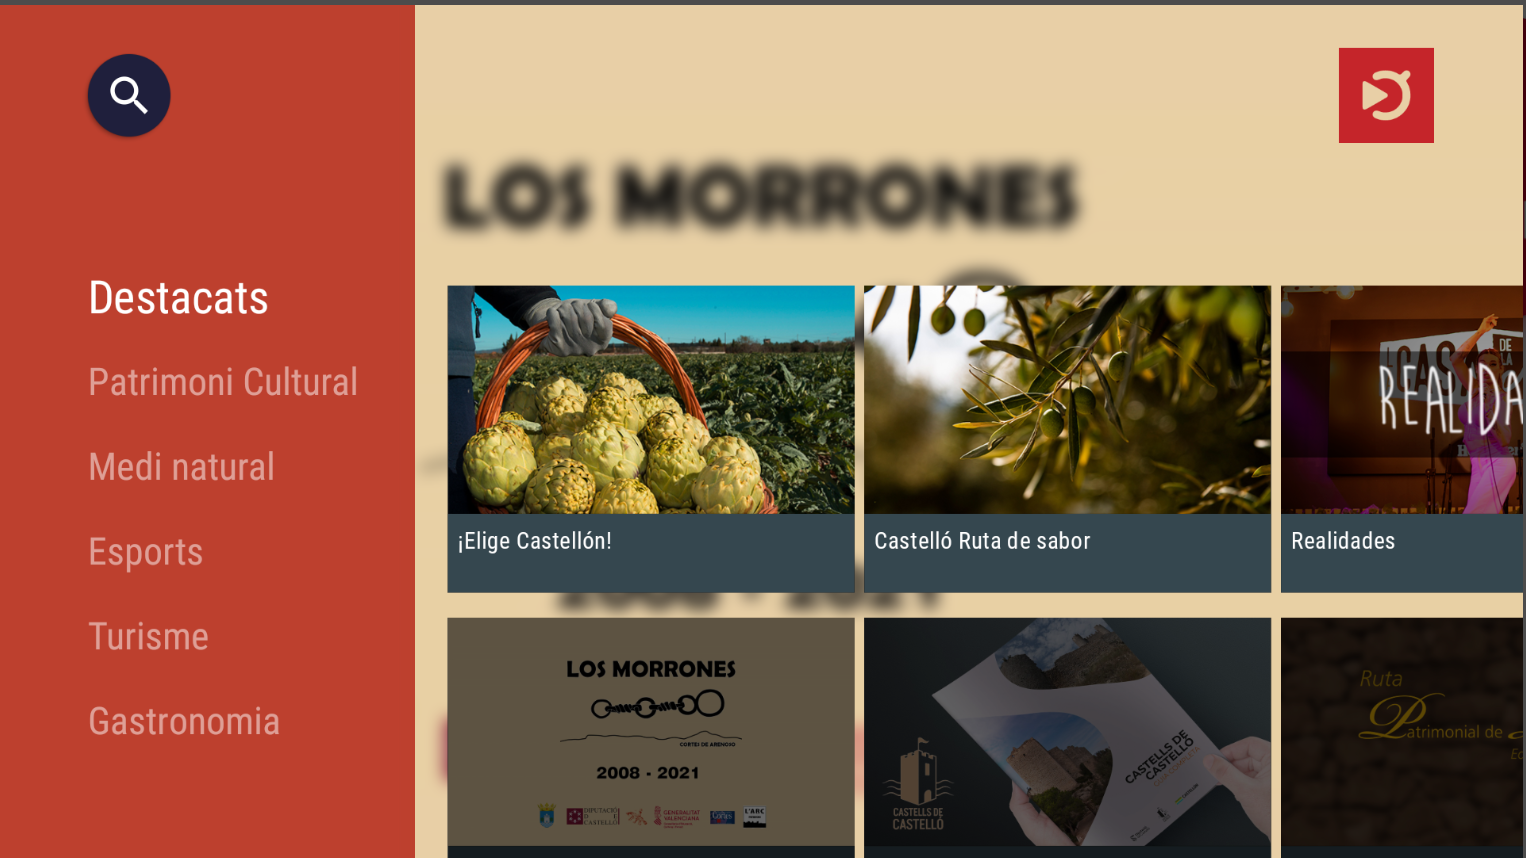
\includegraphics[width=0.8\textwidth]{imaxes/UX_inicios.png}
    \caption{Captura de la interfaz en las primeras fases del proyecto}
    \label{fig:UX_inicios}
\end{figure}
\begin{figure}[H]
    \centering
    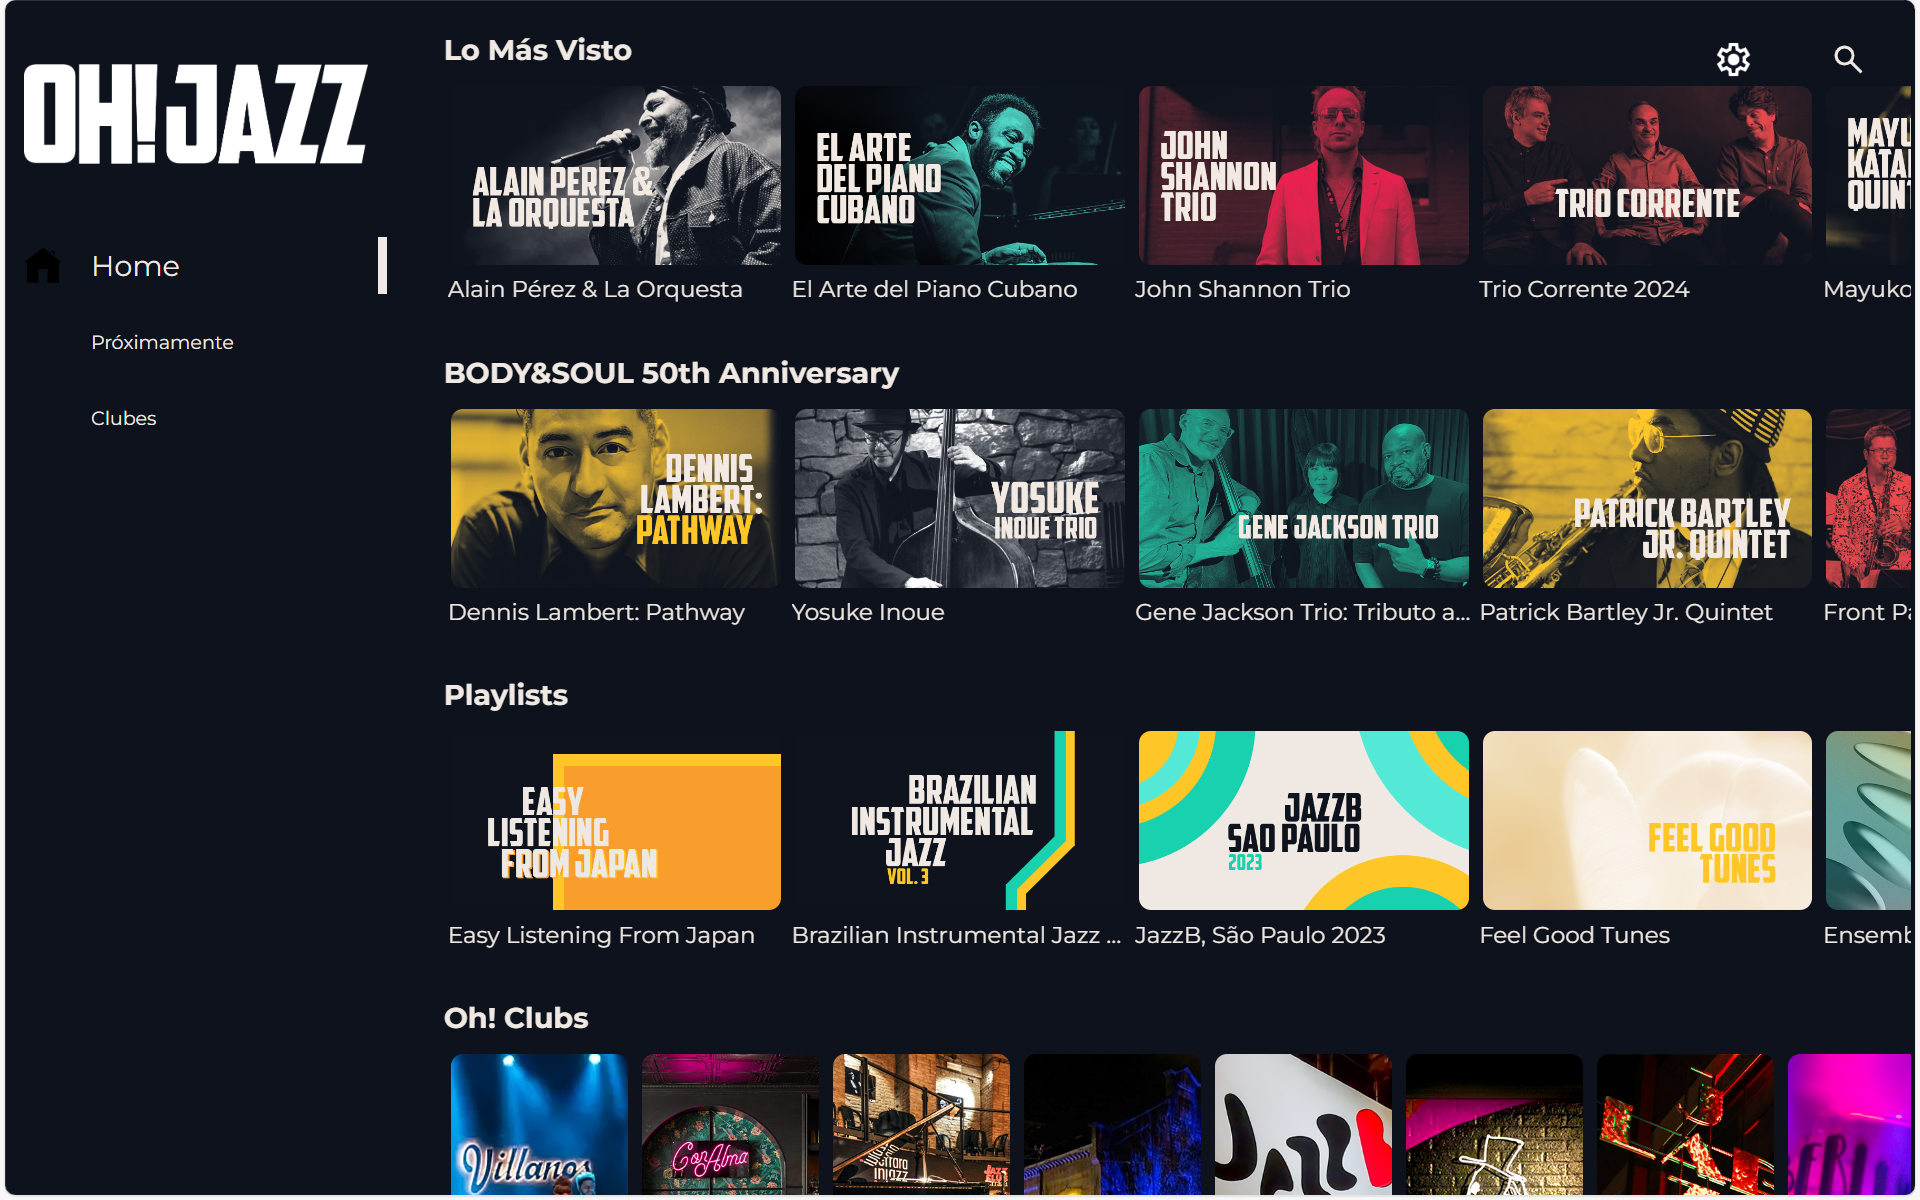
\includegraphics[width=0.8\textwidth]{imaxes/Home_desp_OhJazz.png}
    \caption{Captura de la interfaz más reciente, aún en pruebas por parte del cliente}
    \label{fig:Home_desp_OhJazz}
\end{figure}
\begin{figure}[H]
    \centering
    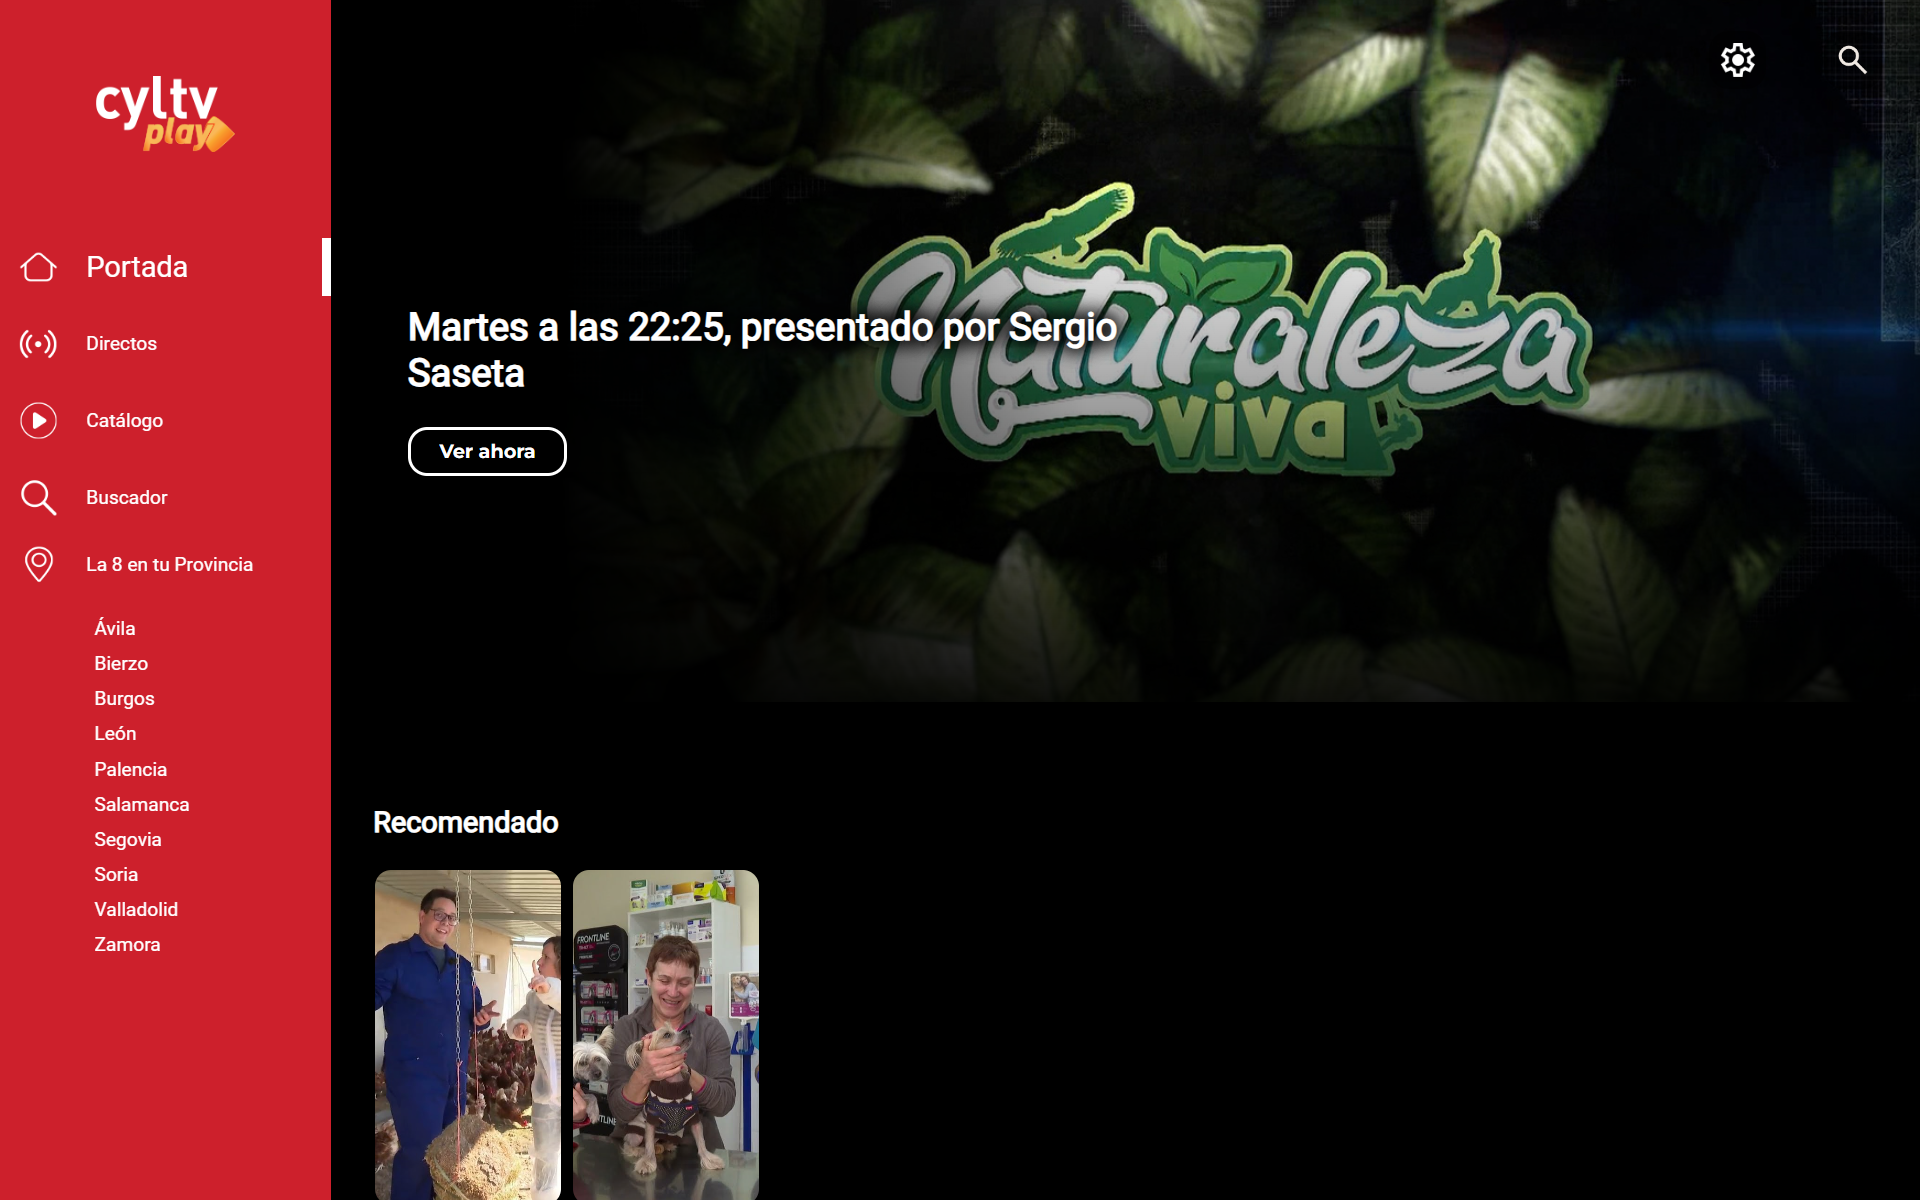
\includegraphics[width=0.8\textwidth]{imaxes/Home_CyLTv.png}
    \caption{Captura de la interfaz casi final}
    \label{fig:Home_CyLTv}
\end{figure}

Estas imágenes muestran la evolución de la interfaz de usuario de \textit{Ott}. La primera imagen refleja el diseño básico inicial, 
sin apenas funcionalidades. En la segunda, se observa un diseño más avanzado, aunque el cliente aún estaba ajustando parámetros (por ejemplo, 
la falta de visibilidad de los iconos de los menús o el contraste del fondo). Finalmente, la tercera imagen muestra la interfaz casi 
final, con un diseño pulido y todas las funcionalidades implementadas.

Más que enfocarse en un diseño único, el proyecto se ha centrado en el diseño de componentes y sus variantes. Algunos elementos de 
la interfaz tienen una estructura fija, aunque permiten personalizar colores y textos:

\begin{itemize}
    \item \textbf{Menú lateral:} Permite navegar por las secciones de la aplicación y se encuentra a la izquierda de la pantalla.
    \item \textbf{Menú superior:} Proporciona acceso a las opciones de configuración. Los iconos y colores de fondo son personalizables, pero la posición depende del número de opciones del menú.
    \item \textbf{Barra de búsqueda:} Situada en la pantalla de búsqueda, su posición y tamaño son fijos, pero utiliza los colores base del cliente para los efectos de foco y difuminado.
    \item \textbf{Lista de elementos:} Muestra los elementos disponibles en la aplicación. La estructura y tamaños son fijos, aunque el contenido y número de listas pueden personalizarse.
    \item \textbf{Detalle de elemento:} Muestra la información detallada de un elemento. Aunque la metadata y el contenido son personalizables, la estructura y disposición de los elementos son fijos. Se está trabajando para permitir mayor personalización desde el gestor de contenidos.
\end{itemize}

El cliente puede personalizar la interfaz ajustando colores de fondo, texto, botones, foco y añadiendo sus logos e imágenes, adaptando la 
aplicación a su identidad visual.
\subsubsection{Personalización de los componentes}
\label{sec:diseno-ux-personalizacion}

Como se ha mencionado anteriormente, el diseño de la interfaz de usuario se ha centrado en la creación de componentes y sus múltiples variantes. 
Estos componentes se dividen en dos tipos principales: \textit{contenidos} y \textit{contenedores}, cada uno de los cuales tiene un enfoque de 
diseño diferente dependiendo del tipo de \textit{widget} en el que se utilicen. Un \textit{widget} es un componente de la interfaz que almacena y 
muestra uno o varios contenidos de manera específica.

Cada tipo de \textit{widget} determina la presentación tanto de los contenidos como de los contenedores, lo que implica que se necesita un diseño y 
un código específico para asegurar que se muestren correctamente en la interfaz. A continuación, se detallan los aspectos clave que cambian según 
el tipo de \textit{widget}:

\begin{itemize}
    \item \textbf{Disposición de los contenidos:} Según el tipo de \textit{widget}, los contenidos se distribuyen de formas diversas. Si se trata de 
    un \textit{widget} de \textbf{destacados}, los contenidos se mostrarán con un tamaño más grande y ocuparán la parte superior de la pantalla, 
    siendo más llamativos. Estos \textit{widgets} pueden tener distintas configuraciones, como la inclusión de botones, un único contenido 
    destacado o varios en formato \textit{slider}, con opciones de distribución de texto e iconos. En contraste, un \textbf{mosaico} organizará los 
    contenidos de manera compacta en el centro de la pantalla. Para otros tipos de \textit{widgets}, como las listas horizontales, los contenidos 
    se dispondrán en filas secuenciales. Estos formatos son personalizables según las necesidades del cliente y el tipo de contenido que se desee resaltar.
    
    \item \textbf{Disposición de la información:} La cantidad y el tipo de información que se muestra también dependen del \textit{widget}. Por ejemplo, 
    en un \textbf{destacado}, el sistema puede mostrar el título, una descripción detallada y un botón de acceso al contenido. En un \textbf{banner}, 
    solo se mostrará el título del contenido. Esta flexibilidad en la información permite que los \textit{widgets} se ajusten a diferentes escenarios 
    y preferencias del cliente, lo que es clave para mantener una interfaz adaptable y eficaz.
    
    \item \textbf{Forma de las imágenes:} La forma y el tamaño de las imágenes asociadas a los contenidos varían según el tipo de \textit{widget}. 
    En los \textbf{destacados}, las imágenes suelen ser grandes, ocupando una buena parte de la pantalla, y pueden cambiar la distribución de la 
    información según el caso específico. En los \textbf{banners}, las imágenes tienen una orientación horizontal con un ratio de 16:9, mientras 
    que en los \textbf{posters}, las imágenes son verticales, con un ratio de 9:16. En los \textbf{posters}, las imágenes aparecen en un panel 
    lateral cuando el foco se mantiene en el contenido durante más de un segundo. Este enfoque garantiza una presentación visual coherente que 
    varía según el tipo de contenido y el diseño del \textit{widget}.
    
    \item \textbf{Otras características:} Algunos \textit{widgets} permiten funcionalidades adicionales que dependen del tipo de contenido que se esté 
    presentando. Por ejemplo, en los \textit{widgets} para contenidos en directo, puede aparecer una barra de progreso y el nombre del programa actual. 
    En un \textbf{widget banner-click}, diseñado para mostrar anuncios, se presenta un banner horizontal que ocupa casi todo el ancho de la pantalla, 
    y al hacer clic en él (excepto en televisores, donde esta opción está desactivada), redirige al usuario a una URL externa.
\end{itemize}

Estas personalizaciones, junto con otras más específicas o en desarrollo, deben estar correctamente implementadas y soportadas por la aplicación 
para garantizar que los \textit{widgets} seleccionados por el cliente funcionen sin problemas y no interfieran con el resto de la interfaz.

Adicionalmente, es importante tener en cuenta ciertas limitaciones en la personalización. Solo puede haber un \textit{widget destacado} por 
pantalla, los \textit{widgets} tipo \textbf{mosaico} con muchos elementos pueden sobrecargar la interfaz, y los \textbf{posters} se utilizan generalmente 
para destacar ciertos contenidos, mostrando información detallada sobre estos.

\subsubsection{Ejemplos de personalización}
\label{sec:diseno-ux-ejemplos}

A continuación se muestran algunos ejemplos de personalización de los widgets de la interfaz de usuario de \textit{Ott}.


\begin{figure}[H]
    \begin{subfigure}[c]{0.5\textwidth}
        
\includegraphics[width=\textwidth]{imaxes/Widget_banner.png}
        \subcaption{Ejemplo de un widget básico de tipo "banner"}
        \label{fig:Widget_banner}
    \end{subfigure}
    \hspace{0.1\textwidth}
    \begin{subfigure}[c]{0.5\textwidth}
        
\includegraphics[width=0.8\textwidth]{imaxes/Widget_destacado.png}
        \subcaption{Ejemplo de un widget básico de tipo "destacado"}
        \label{fig:Widget_destacado}
    \end{subfigure}
    \caption{Ejemplos de un widget básico de tipo "banner" y "destacado"}
    \label{fig:Widget_banner_destacado}
\end{figure}

\begin{figure}[H]
    \begin{subfigure}[c]{0.5\textwidth}
        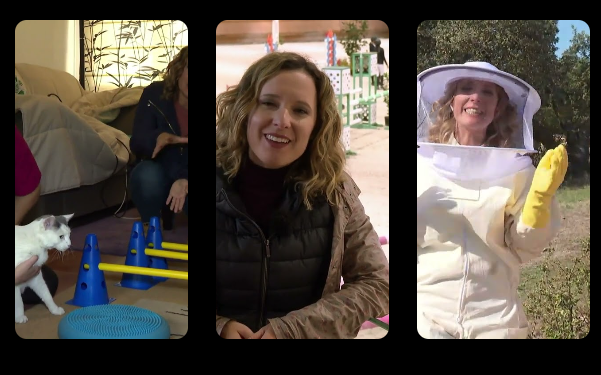
\includegraphics[width=\textwidth]{imaxes/Widget_poster.png}
        \subcaption{Ejemplo de un widget básico de tipo "poster"}
        \label{fig:Widget_poster}
    \end{subfigure}
    \hspace{0.1\textwidth}
    \begin{subfigure}[c]{0.5\textwidth}
        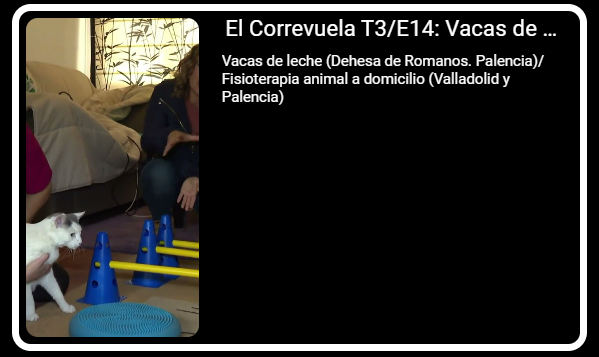
\includegraphics[width=\textwidth]{imaxes/Widget_poster_abierto.png}
        \subcaption{Ejemplo de un widget básico de tipo "poster" con la información mostrada}
        \label{fig:Widget_poster_abierto}
    \end{subfigure}
    \caption{Ejemplos de un widget básico de tipo "poster"}
    \label{fig:Widgets_poster}
\end{figure}


\subsection{Disgramas UML}
\subsection{Introducción}
\label{subsec:Analisis_introduccion}

Una vez completada una fase de análisis y claros los requisitos y objetivos del proyecto, vamos a trabajar sobre 
estos para definir las estructuras de datos, las funciones y los comportamientos del sistema. Se trata de una
fase previa a la implementación, en la que se definen los elementos que compondrán el sistema y cómo se relacionan
entre sí. 

En este apartado se describirá como fueron las primeras fases de diseño de las aplicaciones \textit{Ott} y \textit{Ott Data} 
y como se se trabaja en general en las fases de diseño de nuevas funcionalidades e iteracciones en el proyecto.


\subsection{Estudio y diseño de la aplicación de análisis de datos}
\label{sec:diseno-estudio}

\subsubsection{Diseño general}
\label{sec:diseno-general}

El diseño de la aplicación de análisis de datos se ha realizado siguiendo una metodología de diseño centrada en el usuario. 
Para ello, se ha realizado un análisis de las necesidades de los usuarios, se han definido los requisitos de la aplicación 
y se ha diseñado la interfaz de usuario.

Dentro de las necesidades de los usuarios y de los requisitos de la aplicación se destaca la necesidad de que la visualización
de los datos sea clara y sencilla y que para utilizar la aplicación no sea necesario tener conocimientos avanzados de análisis de datos.

En cuanto al diseño de la interfaz de usuario, se ha optado por un enfoque sencillo y minimalista, utilizando colores suaves y 
una tipografía clara y legible. La interfaz ha sido diseñada para ser intuitiva y fácil de usar, permitiendo al usuario acceder 
rápidamente a todas las funcionalidades de la aplicación. El diseño se centra en la visualización de gráficos y datos, presentando 
la información de manera ordenada y consistente, para que el usuario pueda comprenderla rápidamente. Todas las gráficas y tablas 
comparten un estilo uniforme y limpio, evitando elementos recargados que puedan distraer la atención.

De forma similar a la OTT, el diseño de la aplicacion de análisis de datos se ha realizado siguiendo un enfoque modular,
dividiendo la aplicación en diferentes componentes independientes que se comunican entre sí. Esto permite que la aplicación sea
más fácil de mantener y extender, ya que cada componente puede ser modificado o reemplazado sin afectar al resto de los componenetes 
ni a la interfaz. Además, el diseño modular facilita la reutilización de código y la integración de nuevas funcionalidades.

\subsubsection{Estudio de las agrupaciones de datos}
\label{sec:diseno-agrupaciones}

Una vez definidos los requisitos de la aplicación y el diseño general, era importante estudiar que agrupaciones de datos 
se podian lograr con las funcionalidades que ofrece Matomo y que opciones de visualización se podían implementar. 

Lo primero fue detectar que tipos de gráficos eran necesarios soportar y diseñar. Tras un análisis de la entrega de los datos
que hace Matomo se decidió comenzar con el soporte para gráficos lineales, de barras, circulares y tablas. Así, en función 
de la utilidad, periodo y enfoque de los datos, se podrán seleccionar diferentes tipos de gráficos para visualizar la información.

\paragraph{Páginas y secciones}
Lo siguiente era estudiar que páginas o apartados de la aplicación de análisis de datos se podían implementar. La primera página en la que 
se pensó fue la página de inicio o dashboard, en la que se mostrarán los gráficos que presenten una información más general y resumida
de los datos. 

Otra página en la que se pensó durante el análisis fue una página que permitiera al usuario comparar gráficas provenientes de diferentes
módulos. La idea era que el cliente tuviera la oportunidad de comparar varias gráficas de diferentes módulos en una misma página para 
poder analizar la información en busca de patrones, tendencias o correlaciones entre los datos.

El resto de páginas son dedicadas a agrupaciones de datos que tienen relación entre sí. La creación de estas páginas se enfocó en 
que fuera más dinámica y que permitiera la creación fácil y rápida de nuevas secciones. 



\section{Metodología de Desarrollo}
\label{sec:metodologia_desarrollo}

El desarrollo de la plataforma OTT se llevó a cabo siguiendo una metodología ágil. Esta metodología
permite una mayor flexibilidad en el desarrollo del proyecto, y facilita la adaptación a los cambios
que puedan surgir durante el desarrollo del proyecto. Se asegura así la evolución y mejora controlada
y continua del producto final.

\subsection{Implementacion progresiva e incremental}
\label{subsec:implementacion_progresiva}

El proceso de desarrollo se estructuró en torno a la implementación de funcionalidades de manera 
progresiva e incremental. En lugar de intentar desarrollar todas las características al mismo tiempo, 
el proyecto se dividió en ciclos más pequeños, cada uno enfocado en la entrega de una funcionalidad específica.

Estos ciclos se componen de las siguientes fases:
\begin{itemize}
    \item \textbf{Análisis:} En esta fase se escoge la funcionalidad a implementar y se identifican los 
    requisitos de la misma. La selección de la funcionalidad a implementar se realiza en base a la
    prioridad de la misma y a la dependencia de otras funcionalidades.
    \item \textbf{Diseño:} En esta fase se diseña la arquitectura de la funcionalidad a implementar. Se
    identifican los componentes necesarios y se definen las interacciones entre ellos.
    \item \textbf{Implementación:} En esta fase se implementa la funcionalidad siguiendo el diseño
    previamente definido.
    \item \textbf{Pruebas:} En esta fase se realizan pruebas unitarias y de integración para asegurar
    que la funcionalidad implementada cumple con los requisitos definidos en la fase de análisis.
\end{itemize}

\subsection{Adaptación continua y flexibilidad}
\label{subsec:adaptacion_continua}

Una de las ventajas de la metodología ágil es la adaptación continua y la flexibilidad que ofrece, permitiendo
hacer frente a los cambios y nuevas necesidades que puedan surgir durante el desarrollo del proyecto y ajustar
las prioridades y el enfoque del proyecto en caso de ser necesario.

Durante el desarrollo de la plataforma OTT, se realizaron reuniones periódicas los clientes para revisar
el progreso del proyecto y validar las funcionalidades implementadas. Estos clientes
pudieron proponer cambios y mejoras en la plataforma, que fueron evaluados y estudiados. Debido a la naturaleza
multicliente del proyecto, en todo momento se busco que los cambios o mejoras realizadas en base a peticiones de un 
cliente en específico no afectaran a los demás clientes. Uno de los objetivos principales que tiene el proyecto
es seguir aumentando la flexibilidad y personalización de la plataforma para cada cliente.


\subsection{Reuniones de Validación y Planificación}
\label{subsec:reuniones_validacion}

Después de cada ciclo de desarrollo, se llevaron a cabo reuniones de validación para revisar las 
funcionalidades completadas y planificar las siguientes etapas. Estas reuniones fueron fundamentales 
para asegurar que el proyecto se mantuviera alineado con los objetivos del cliente y para permitir la 
rápida adaptación a nuevos requisitos. En estas sesiones, se discutía el estado actual del proyecto, 
se evaluaban posibles mejoras, y se decidía la próxima funcionalidad a implementar. Este enfoque 
colaborativo garantizó una toma de decisiones informada y una respuesta rápida a los cambios necesarios.


\subsection{Ventajas de la metodología ágil}
\label{subsec:ventajas_agil}

La metodología ágil ofrece una serie de ventajas que permiten un desarrollo más eficiente y controlado del proyecto.
Algunas de las ventajas más destacadas son las siguientes:

\begin{itemize}
    \item \textbf{Mayor flexibilidad:} La metodología ágil permite adaptarse a los cambios y nuevas necesidades
    que puedan surgir durante el desarrollo del proyecto.
    \item \textbf{Mayor control:} Al dividir el proyecto en ciclos más pequeños, se facilita el seguimiento y
    control del progreso del proyecto.
    \item \textbf{Mayor calidad:} Al realizar pruebas continuas a lo largo del desarrollo del proyecto, se asegura
    que el producto final cumple con los requisitos y está libre de errores.
    \item \textbf{Mayor satisfacción del cliente:} Al involucrar al cliente en el proceso de desarrollo y permitirle
    proponer cambios y mejoras, se asegura que el producto final cumple con sus expectativas.
\end{itemize}
\section{Descripción de las Etapas de Desarrollo}
En esta sección, se describen las principales etapas del desarrollo del proyecto, 
desde la planificación inicial hasta el despliegue final. Cada etapa jugó un papel 
crucial en la evolución del proyecto, permitiendo una implementación organizada y eficiente de la plataforma OTT.

\subsection{Fase de Análisis y Planificación}
\subsubsection{Recolección de Requisitos}
En esta etapa, se realizó un análisis exhaustivo para identificar los requisitos 
funcionales y no funcionales del proyecto. Esto incluyó reuniones con los clientes
para entender las expectativas y necesidades de cada uno, así como un análisis de mercado para
asegurar que las plataformas cumplieran con los estándares actuales. 

\subsection{Fase de Diseño}
\subsubsection{Diseño de Arquitectura}
Durante esta etapa, se definió la arquitectura general de la plataforma  OTT con sus componentes. Se utilizó 
una arquitectura basada en microservicios para garantizar la escalabilidad y flexibilidad del 
sistema e integración con los servicios existentes en la empresa. También se diseñó la estructura de 
comunicación entre los componentes y se eligieron las tecnologías más adecuadas para cada parte del sistema.

Se estudiarón los conjuntos de datos y las APIs necesarias para creación de la plataforma de análisis de datos.

\subsubsection{Diseño de la Interfaz de Usuario}
Se comenzó a trabajar sobre una interfaz básica para la plataforma OTT que permitiera el desarrollo de las funcionalidades
principales de la plataforma y poco a poco se fue refinando y mejorando en función de las peticiones
de los clientes y las pruebas de usabilidad realizadas. A través de reuniones con los clientes y 
analizando sus peticiones y prototipos, se fueron contruyendo los diseños de manera conjunta hasta
llegar a un diseño final que satisfaciera las necesidades de los usuarios.

Se diseño la interfaz de usuario para la plataforma de análisis de datos, con el objetivo de que los usuarios
pudieran visualizar y analizar los datos de manera sencilla y efectiva sin necesidad de conocimientos técnicos.

\subsection{Fase de Desarrollo}
\subsubsection{Implementación de Funcionalidades}
Esta fase fue el núcleo del proyecto, donde se desarrollaron las funcionalidades clave de la 
plataforma OTT. Cada funcionalidad se implementó de manera incremental, siguiendo un ciclo 
ágil de análisis, diseño, codificación y pruebas. Se utilizaron tecnologías web como JavaScript, 
HTML y CSS para asegurar la compatibilidad multiplataforma.

Para la plataforma de análisis de datos, se implementaron las funcionalidades necesarias para
la carga, procesamiento y visualización de los datos, así como de análisis y generación de informes.

\subsubsection{Optimización y Refactorización}
A medida que se añadían nuevas funcionalidades, el código se refactorizaba y optimizaba para 
mejorar el rendimiento y la mantenibilidad. Este proceso incluyó la simplificación de la lógica 
de negocio, la mejora de la estructura del código, y la optimización de la carga y la respuesta de la aplicación.

\subsection{Fase de Pruebas}
\subsubsection{Pruebas Unitarias y de Integración}
Se realizaron pruebas unitarias para cada componente, asegurando que las funciones individuales 
funcionaran correctamente. Luego, se realizaron pruebas de integración para verificar que los 
componentes interactuaran de manera efectiva y sin conflictos.

\subsubsection{Pruebas de Compatibilidad}
Se llevaron a cabo pruebas exhaustivas en diferentes dispositivos y sistemas operativos 
(web, Tizen, WebOS, Android TV) para asegurar que la aplicación funcionara correctamente 
en todos los entornos previstos. Esto incluyó pruebas de rendimiento para garantizar que 
la aplicación se ejecutara sin problemas en dispositivos con capacidades de hardware limitadas.


\subsection{Conclusión}	  
Estas etapas se llevaron a cabo de manera iterativa y colaborativa, con reuniones periódicas
con los clientes para validar el progreso y ajustar las prioridades según fuera necesario.
Así para cada funcionalidad nueva se realizaba un ciclo de análisis, diseño, implementación y pruebas
para asegurar que la funcionalidad cumpliera con los requisitos y expectativas del cliente.


\section{Diagrama de Gantt}
El diagrama de Gantt de la Figura \ref{fig:gantt_chart} muestra la planificación de las etapas del proyecto, 
desde el análisis de viabilidad hasta la entrega final. Cada proyecto se distingue por un color diferente, y 
cada etapa se representa con un tono distinto para facilitar la diferenciación entre las fases.

\begin{figure}[H]
  \centering
  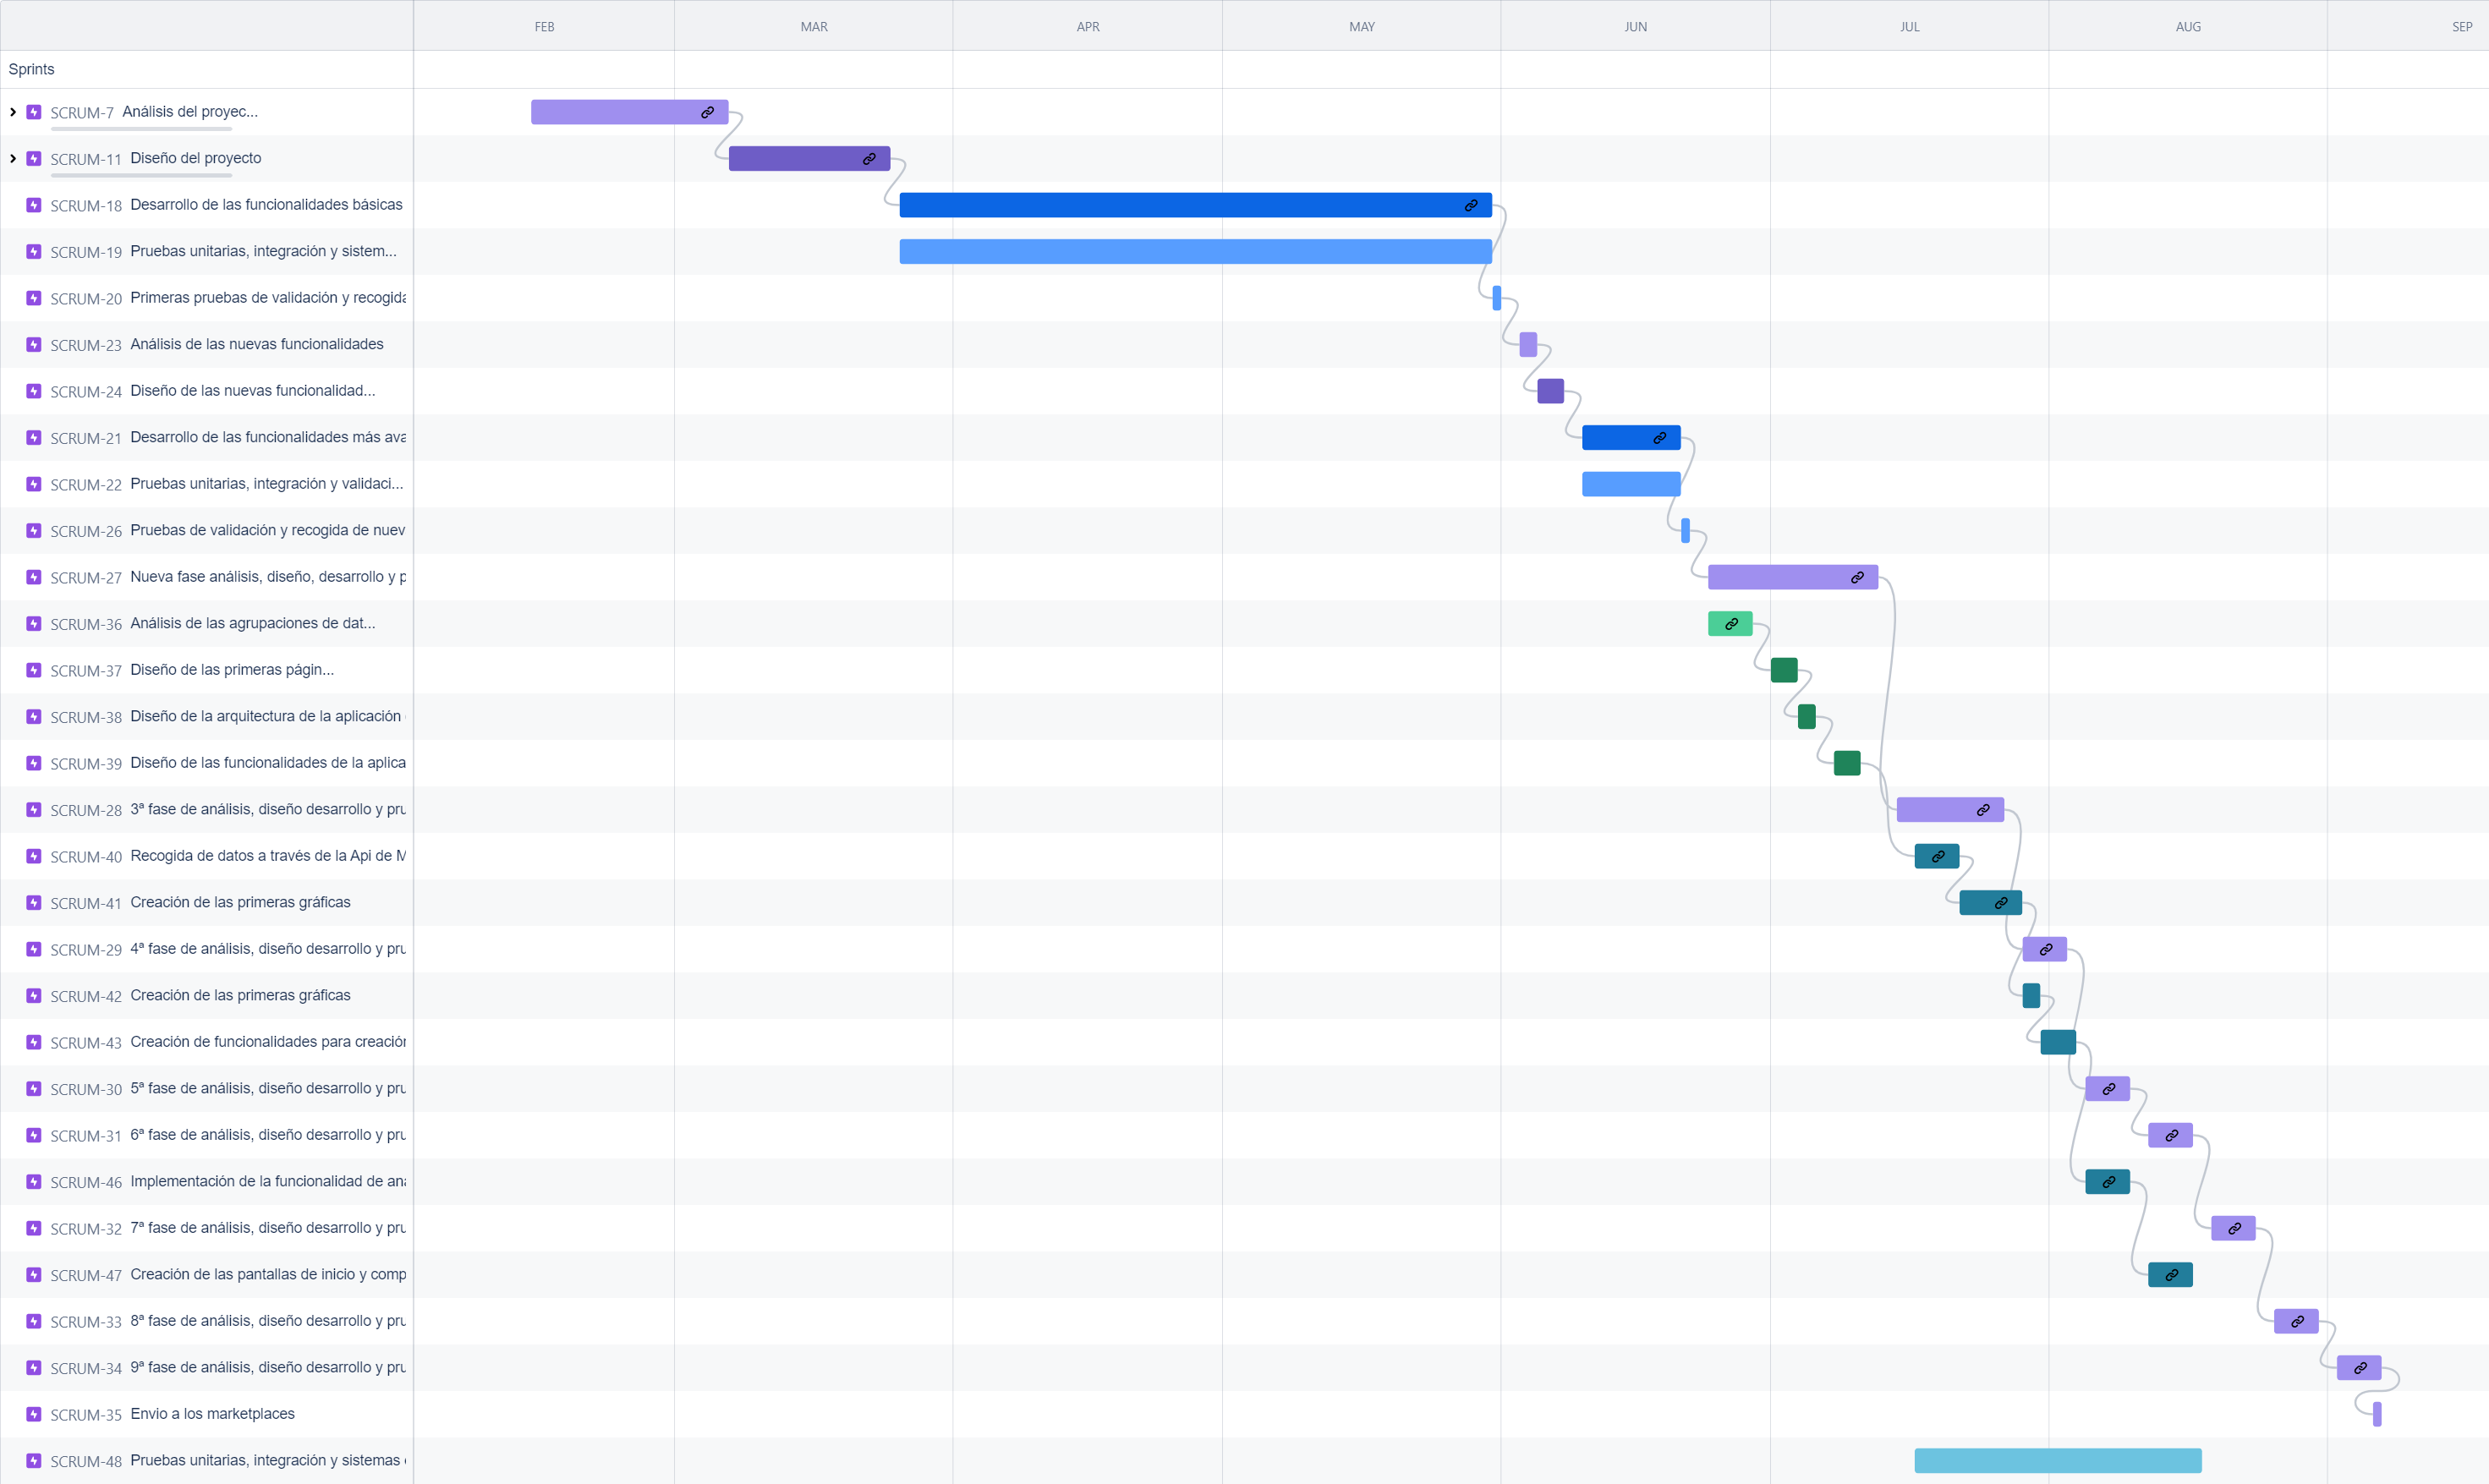
\includegraphics[width=0.9\textwidth]{imaxes/gantt_chart}
  \caption{Diagrama de Gantt del Proyecto}
  \label{fig:gantt_chart}
\end{figure}

Como se puede apreciar en la Figura \ref{fig:gantt_chart}, el proyecto se dividió en varias etapas, cada una 
de ellas con tareas y subetapas asignadas. La planificación de cada etapa se estableció para un tiempo determinado, 
y se llevaron a cabo reuniones periódicas para evaluar el progreso y realizar los ajustes necesarios en la planificación.

Cada etapa está compuesta por:
\begin{itemize}
    \item Una fase de \textbf{análisis}, donde se evaluaban los requisitos y las posibles soluciones.
    \item Una fase de \textbf{diseño}, en la que se definían los detalles técnicos y de la interfaz.
    \item Una fase de \textbf{desarrollo}, que involucraba la implementación de las funcionalidades y optimización de las mismas.
    \item Una fase de \textbf{pruebas}, que incluía la validación de la funcionalidad y la realización de ajustes según fuera necesario.
\end{itemize}

Se realizaron reuniones periódicas con los clientes para validar el progreso y ajustar las prioridades conforme avanzaba el proyecto.

\paragraph{Explicación detallada del diagrama de Gantt:}

\begin{enumerate}
    \item \textbf{Análisis del Proyecto:} La primera etapa incluyó el análisis de viabilidad y la planificación de las fases iniciales. 
    Esto permitió definir claramente los objetivos y establecer un calendario preliminar para el resto del desarrollo.
   
    \item \textbf{Diseño del Proyecto:} Se desarrolló la estructura básica y se realizaron los primeros bocetos de la 
    interfaz de usuario y la arquitectura de microservicios. Este paso fue fundamental para asegurar que el diseño fuera 
    escalable y adaptable a las diferentes plataformas.

    \item \textbf{Desarrollo de Funcionalidades Básicas:} Una vez que se establecieron las bases del diseño, comenzó el desarrollo 
    de las funcionalidades clave de la plataforma OTT y la plataforma de análisis de datos.

    \item \textbf{Pruebas Unitarias e Integración:} Durante todo el proceso, las funcionalidades fueron sometidas a pruebas para 
    asegurar que todas las partes del sistema funcionaran correctamente antes de proceder con nuevas implementaciones.

    \item \textbf{Validaciones y Mejoras Continuas:} Se realizó una validación constante de las funcionalidades mediante pruebas 
    de usuario y reuniones con los clientes. También se ajustaron las funcionalidades según la retroalimentación recibida.

    \item \textbf{Despliegue Final y Entrega:} En la última etapa, se realizaron pruebas finales en los marketplaces y se preparó 
    la aplicación para su lanzamiento, asegurando que cumpliera con los requisitos de las distintas plataformas y que estuviera 
    lista para ser publicada.
\end{enumerate}

Como se muestra en el diagrama de Gantt, las fases de diseño, desarrollo y pruebas están interconectadas, con dependencias claras 
que marcan cómo cada tarea debía completarse antes de avanzar a la siguiente. Esto permitió un seguimiento detallado del progreso 
y facilitó la identificación de posibles retrasos o áreas que requerían ajustes.


  \chapter{Análisis}
\label{chap:analisis}

\section{Introducción}
\label{sec:analisis_introduccion}

El análisis es la primera fase del ciclo de vida de un proyecto de software. En esta fase se recopilan los requisitos 
del sistema, se identifican los objetivos y se establecen las restricciones que debe cumplir el sistema. 
El análisis es una fase crucial en el desarrollo de software, ya que de ella depende el éxito o fracaso del proyecto. 
En esta fase se establece la base sobre la que se construirá el sistema, por lo que es importante que se realice de forma correcta y exhaustiva.

En esta sección se describirá como se ha realizado el análisis del proyecto, los objetivos que se pretenden alcanzar y las restricciones que se han establecido.


\section{Requisitos}
\label{sec:analisis_requisitos}

En software, se entiende por requisito a una condición o capacidad que debe cumplir un sistema para
resolver un problema o satisfacer una necesidad. Son las funciones, características y restricciones que
debe cumplir un producto final.

La identificación de requisitos es una etapa crucial en cualquier proyecto software ya que marca el
camino a seguir en el desarrollo del sistema. Si no se identifican correctamente los requisitos, el
sistema no trabajará correctamente y no cumplirá ni sus especificaciones ni las expectativas del
cliente. Por ello, es importante que los requisitos sean claros, precisos y completos. 

Para hacer una correcta identificación de los requisitos, hay que tener en cuenta y conoces los 
dos tipos de requisitos que nos podemos encontrar: los requisitos funcionales, que describen las
funciones que debe realizar el sistema, y los requisitos no funcionales, que describen las
características que debe tener el sistema. 

Además, es importante conoces de donde se deben obtener los requisitos. Si leemos el apartado 
7.2 de la norma ISO 9001:2000, Realización del producto. Procesos relacionados con el cliente, 
este nos dice que los requisitos relativos se obtienen de: 

\begin{itemize}
    \item Los requisitos especificados por el cliente.
    \item Requisitos no especificados por el cliente pero necesarios para el uso especificado o
    para el uso previsto, cuando sea conocido.
    \item Requisitos legales y reglamentarios relacionados con el producto.
    \item Requisitos adicionales determinados por la organización.
\end{itemize}

Todo los requisitos que se detecten en esta fase deben ser revisados por la organización para 
asegurarse de que son correctos, completos, se entienden y pueden ser suministrados. Este proceso
de revisión debe llevarse a cabo a lo largo de todo el proyecto cuando alguno de estos requisitos
sufra alguna modificación.

\subsection{Requisitos de la plataforma OTT}
\label{subsec:analisis_requisitos_plataforma_ott}

En esta sección se describirán los requisitos recogidos para la plataforma OTT. Los requisitos detallados a 
continuación son los relacionados con la creación de la aplicación multiplataforma y multicliente, que recibe
la información y determina como mostrar esta. Dentro de estos requisitos no se incluyen los relacionados 
con otros componentes de la plataforma, como la CDN, la gestión de usuarios, la gestión de contenidos, etc.

\subsubsection{Requisitos funcionales}
\label{subsubsec:analisis_requisitos_funcionales}

\paragraph{Requisitos especificados por el cliente}
\label{par:analisis_requisitos_funcionales_cliente}

En este caso los requisitos no son unicamente de un cliente, sino que como ya se ha comentado
en la introducción, se han recogido los requisitos de varios clientes. Ejemplos de requisitos
especificos de clientes:

\paragraph{Generales}
\label{par:analisis_requisitos_funcionales_generales}

\begin{itemize}
    \item El usuario debe tener una pantalla donde poder buscar contenido.
    \item El usuario debe disponer de una pantalla con los ajustes de la aplicación.
\end{itemize}

\paragraph{Radio Television de Castilla y León. CyLTv Play}
\label{par:analisis_requisitos_funcionales_cyltvplay}

\begin{itemize}
    \item El usuario debe tener disponible una pantalla donde se muestre todo el contenido en directo.
    \item El usuario debe tener disponible una pantalla donde se muestre todo el contenido a la carta.
    \item El usuario debe tener una pantalla disponible para cada delegación del canal La 8.
\end{itemize}

\paragraph{Oh!Jazz}
\label{par:analisis_requisitos_funcionales_ohjazz}

\begin{itemize}
    \item El usuario debe poder iniciar y cerrar sesión.
    \item Los usuarios no loggeados no pueden acceder a todos los contenidos.
    \item El usuario debe poder cambiar de idioma la plataforma.
\end{itemize}

\paragraph{Requisitos no especificados por el cliente}
\label{par:analisis_requisitos_funcionales_no_cliente}

Este tipo de plataformas tienen unos requisitos comunes que no han sido especificados por los clientes,
pero que son necesarios para el correcto funcionamiento de la plataforma. Estos requisitos son:

\begin{itemize}
    \item La interfaz debe recibir la información necesaria para saber qué y cómo mostrar los contenidos.
    \item La aplicación debe ser capaz de determinar, para que cliente está trabajando y tomar decisiones 
    en función de esto.
    \item La aplicación debe ser capaz de determinar, para que plataforma está trabajando y tomar decisiones
    en función de esto.
    \item La aplicación debe crear una interfaz de usuario que sea atractiva, intuitiva y fácil de usar.
    \item La aplicación debe crear una interfaz que se adapte a distintas resoluciones.
    \item La aplicacion debe ser capaz de reproducir los contenidos multimedia en cualquier sistema operativo.
    \item La aplicación debe estar personalizada con los logos y colores de cada cliente.
    \item La aplicación debe funcionar con los botones del mando a distancia en el caso de las televisiones.
    \item La aplicación debe mostrar los datos correctamente sin alterar la información.
\end{itemize}

\subsubsection{Requisitos no funcionales}
\label{subsubsec:analisis_requisitos_no_funcionales}

\paragraph{Requisitos de rendimiento}
\label{par:analisis_requisitos_no_funcionales_rendimiento}

\begin{itemize}
    \item La aplicación debe ser capaz de mostrar los contenidos en el menor tiempo posible.
    \item La aplicación debe ser capaz de reproducir los contenidos multimedia sin cortes.
    \item La experiencia de usuario debe ser lo más fluida posible.
    \item La aplicación debe ser capaz de adaptarse a distintas resoluciones.
\end{itemize}

\paragraph{Requisitos de seguridad}
\label{par:analisis_requisitos_no_funcionales_seguridad}

\begin{itemize}
    \item La aplicación debe ser segura y no permitir accesos no autorizados.
    \item La aplicación debe proteger los datos de los usuarios.
    \item La aplicación debe proteger los datos de los clientes.
\end{itemize}

\paragraph{Requisitos de usabilidad}
\label{par:analisis_requisitos_no_funcionales_usabilidad}

\begin{itemize}
    \item La aplicación debe ser intuitiva y fácil de usar.
    \item La aplicación debe ser atractiva y agradable visualmente.
    \item La aplicación debe ser accesible para todo tipo de usuarios.
\end{itemize}

\paragraph{Requisitos de mantenimiento}
\label{par:analisis_requisitos_no_funcionales_mantenimiento}

\begin{itemize}
    \item La aplicación debe ser fácil de mantener y actualizar.
    \item La aplicación debe ser fácil de escalar.
    \item La aplicación debe ser fácil de desplegar.
\end{itemize}

\paragraph{Requisitos de escalabilidad}
\label{par:analisis_requisitos_no_funcionales_escalabilidad}

\begin{itemize}
    \item La aplicación debe ser capaz de adaptarse a un aumento de usuarios.
    \item La aplicación debe ser capaz de adaptarse a un aumento de contenidos.
    \item La aplicación debe ser capaz de adaptarse a un aumento de clientes.
\end{itemize}

\paragraph{Requisitos de disponibilidad}
\label{par:analisis_requisitos_no_funcionales_disponibilidad}

\begin{itemize}
    \item La aplicación debe estar disponible en todo momento.
    \item La aplicación debe ser capaz de recuperarse de fallos.
    \item La aplicación debe ser capaz de recuperarse de caídas.
\end{itemize}

\paragraph{Requisitos de compatibilidad}
\label{par:analisis_requisitos_no_funcionales_compatibilidad}

\begin{itemize}
    \item La aplicación debe ser compatible con todos los sistemas operativos.
    \item La aplicación debe ser compatible con todos los navegadores.
    \item La aplicación debe ser compatible con todos los dispositivos.
\end{itemize}

\paragraph{Requisitos de internacionalización}
\label{par:analisis_requisitos_no_funcionales_internacionalizacion}

\begin{itemize}
    \item La aplicación debe ser capaz de adaptarse a distintos idiomas.
    \item La aplicación debe ser capaz de adaptarse a distintas culturas.
    \item La aplicación debe ser capaz de adaptarse a distintas zonas horarias.
\end{itemize}

\paragraph{Requisitos de personalización}
\label{par:analisis_requisitos_no_funcionales_personalizacion}

\begin{itemize}
    \item La aplicación debe ser personalizable con los logos y colores de cada cliente.
    \item La aplicación debe ser personalizable con los logos y colores de cada plataforma.
    \item La aplicación debe ser personalizable con los logos y colores de cada delegación.
\end{itemize}

\paragraph{Requisitos de adaptabilidad}
\label{par:analisis_requisitos_no_funcionales_adaptabilidad}

\begin{itemize}
    \item La aplicación debe ser capaz de adaptarse a distintas resoluciones.
    \item La aplicación debe ser capaz de adaptarse a distintos dispositivos.
    \item La aplicación debe ser capaz de adaptarse a distintos navegadores.
\end{itemize}






\section{Necesidades del cliente}
\label{sec:analisis_necesidades_cliente}

Como se ha comentado en la sección \ref{sec:analisis_requisitos_funcionales}, el analisis de requisitos
en esta aplicación es un tanto especial, ya que no existe un solo cliente sino que existen varios clientes
cada uno con sus necesidades y requisitos. El objetivo del proyecto es satisfacer y cumplir con esos 
requisitos y necesidades a partir de una única aplicación. 

Esto supone que además del estudio de viabilidad técnica, para cada requisito se ha estudiado la manera
de implementarlo de forma que, o bien sirva para todos los clientes, o en caso de ser un requisito 
muy especifico y necesario para un cliente, hacerlo de manera que no afecte al resto de clientes.

Un ejemplo de esto es la interfaz. La interfaz ya cuenta con las funcionalidades necesarias para mostrar
los colores, logos e imagenes de cada cliente. En cuanto a la presentación de los contenidos general, esta es muy similar
en cualquier OTT del mercado: listas horizontales con imagenes y textos de los distintos contenidos. Esto 
no supone ningún problema ya que son los clientes los que gestionan los textos y las imagenes y los responsables
de que estos esten en armonia para una interfaz atractiva. El reto está en elementos del menú dedicados a mostrar
de manera especial los contenidos. Un ejemplo de esto, las listas de destacados. Estas listas son aquellas que se sitúan,
por lo general, en la parte superior de las pantallas y muestran los contenidos más importantes. El problema está en que
cada cliente tiene una idea de como quiere que se muestren estos contenidos. Las opciones de configuración si se quiere
dar libertad al cliente son muchas. El cliente puede decidir si quiere botón de play, si quiere que se muestre el título,
el subtitulo, la duración, la fecha de publicación, etc. Para poder dar soporte a todas estas opciones lo que se ha hecho
es crear un sistema de "etiquetado" o "clasificación" tanto de los contenidos como de las listas en los que se encuentran
estos contenidos. De esta manera, en función del tipo de lista (también conocido como widget) y del tipo de contenido,
estos se mostrarán de una manera u otra. Esto tiene una serie de ventajas y de inconvenientes. Si hablamos de ventajas,
la principal es que cada cliente puede personalizar la interfaz a su gusto, diferenciandose del resto de clientes.
Si hablamos de inconvenientes, el principal es que para cada tipo de lista y de contenido se debe dar soporte en la aplicación.
 Esto supone un esfuerzo extra en el desarrollo y en la gestión de los contenidos. 

 Este ha sido el enfoque que se ha dado a la aplicación desde un principio debido a la arquitectura de los distintos
 componentes creados y del funcionamiento de otras plataformasque pertenecen a la empresa. El enfoque en el que se está 
 trabajando ahora mismo es en una mayor personalización de widgets y contenidos, sin necesidad de tener que crear un nuevo
 tipo de estos elementos cada vez que se requiera una personalización o presentación nueva. Lo mismo para las distintas
 pantallas. 
\section{Estudio de viabilidad}
\label{sec:analisis_estudio_viabilidad}

Desde el inicio, uno de los principales interrogantes fue si era factible desarrollar una aplicación única 
que pudiera generar versiones para distintos sistemas operativos y dispositivos. Este apartado analiza la 
viabilidad técnica y económica del proyecto, abordando las preguntas clave sobre la posibilidad de crear 
una solución híbrida entre dispositivos móviles y televisores, la existencia de tecnologías adecuadas y 
la eficiencia en su implementación.

\subsection{Viabilidad técnica}
\label{subsec:analisis_estudio_viabilidad_tecnica}

La \href{https://es.wikipedia.org/wiki/Viabilidad_t%C3%A9cnica#:~:text=Condici%C3%B3n%20que%20hace%20posible%20el,leyes%20de%20la%20naturaleza%20involucradas.}{viabilidad técnica} 
de un proyecto se refiere a la condición que hace posible llevar a cabo una idea o proyecto desde el punto de 
vista tecnológico. Para evaluar la viabilidad de este proyecto, es crucial determinar si existe una herramienta 
o tecnología que permita trabajar con un número suficiente de sistemas operativos y dispositivos para que el 
proyecto sea rentable. A continuación, se detalla este estudio.

En cuanto a infraestructura, la empresa ya dispone de los componentes necesarios y completamente funcionales 
para soportar la aplicación. Tanto el CMS, como la base de datos y los servidores de aplicaciones están operativos 
y son capaces de manejar la carga de trabajo que la aplicación requerirá, lo que hace que la viabilidad técnica 
en este aspecto sea positiva.

\subsubsection{Adaptación a web}
\label{subsubsec:analisis_estudio_viabilidad_tecnica_aplicacion_web}

Las aplicaciones web ofrecen flexibilidad y portabilidad, permitiendo el uso de diversas tecnologías y 
lenguajes de programación. Este entorno facilita el desarrollo, ya que la aplicación puede aprovechar 
tecnologías comunes para adaptarse a otros dispositivos, sin que la viabilidad técnica sea un obstáculo significativo.

\subsubsection{Adaptación a televisores}
\label{subsubsec:analisis_estudio_viabilidad_tecnica_aplicacion_tv}

El caso de los televisores es muy distinto. Aunque los televisores inteligentes actuales cuentan con un navegador
web, estos no son ni tan potentes ni tan cómodos de utilizar como los de los dispositivos móviles o los ordenadores, 
por lo que, aunque una persona pueda acceder a la aplicación desde su televisor, no es la opción ideal para 
estos dispositivos. La opción que aplica para este proyecto es la de crear una aplicación nativa para televisores.
Estas aplicaciones se ejecutan directamente en el sistema operativo del televisor, lo que requiere compatibilidad
con la tecnología utilizada para desarrollar la aplicación.

Los sistemas operativos que se estudiaron en un primer momento para este proyecto fueron los más utilizados en 
televisores inteligentes: Android TV, Tizen, webOS y Apple TV. La primera opción fue utilizar tecnologías como 
JavaScript, HTML y CSS. Tras analizar Tizen y webOS, se confirmó que ambas opciones permiten el desarrollo con 
estas tecnologías, lo que hacía viable la implementación técnica. Sin embargo, Android TV y Apple TV no permiten 
el desarrollo con estas tecnologías de manera nativa, ya que utilizan sus propios entornos de desarrollo. Para 
superar esta limitación en Android TV, se optó por \href{https://cordova.apache.org/}{Apache Cordova}, una 
herramienta que permite crear aplicaciones híbridas usando HTML, CSS y JavaScript. En el caso de Apple TV, no se 
encontró una solución viable en esta etapa para adaptar el código a sus tecnologías propietarias.

Aunque no se encontró una solución para Apple TV, la capacidad de desarrollar para Android TV, junto con Tizen 
y webOS, cubre aproximadamente un 27\% del mercado mundial de televisores inteligentes \cite{smarttv_marketshare}. 
Aunque no es un porcentaje muy alto, es suficiente para considerar el proyecto como viable.

Con el proyecto ya en marcha y versiones funcionales de la aplicación disponibles, se están estudiando nuevas 
implementaciones para otros sistemas operativos y dispositivos. Entre las opciones futuras está Vidaa OS 
(Hisense), que actualmente posee el 7.8\% del mercado mundial, posicionándose como el segundo sistema operativo 
más utilizado. Los primeros estudios sobre Vidaa OS han sido positivos, indicando que es compatible con las 
tecnologías elegidas, por lo que se planea continuar con el análisis y eventualmente integrar este sistema operativo.

En cuanto a Apple TV, se planifica desarrollarlo por separado y explorar cómo adaptar el código de la aplicación 
a su tecnología en el futuro, si es posible.

\subsubsection{Adaptación a dispositivos móviles}
\label{subsubsec:analisis_estudio_viabilidad_tecnica_aplicacion_movil}

Inicialmente, el enfoque no está en generar aplicaciones móviles nativas, sino en asegurar que la página web 
sea responsive para ofrecer una buena experiencia en dispositivos móviles. A medio plazo, se contempla la 
posibilidad de desarrollar para Android, con una probable exclusión inicial de iOS debido a las limitaciones tecnológicas.

\subsubsection{Conclusión}
\label{subsubsec:analisis_estudio_viabilidad_tecnica_conclusion}

El proyecto es técnicamente viable. A pesar de la limitación con Apple TV, el soporte para Android TV, Tizen 
y webOS, junto con la flexibilidad del desarrollo web, asegura que el proyecto puede avanzar con éxito.

\subsection{Viabilidad económica}
\label{subsec:analisis_estudio_viabilidad_economica}

La viabilidad económica se centra en evaluar los costos y beneficios del proyecto para determinar su rentabilidad.

\subsubsection{Costes}
\label{subsubsec:analisis_estudio_viabilidad_economica_costes}
Los costes que conlleva el desarrollo de este proyecto son los siguientes:

\begin{itemize}
    \item \textbf{Costes de desarrollo:} Incluyen el desarrollo de la aplicación, donde el único gasto significativo ha sido 
    el del desarrollador, ya que muchas herramientas y sistemas de prueba son gratuitos o ya existentes. Otros gastos, 
    como diseñadores o licencias, han sido cubiertos por los clientes.
    
    \item \textbf{Costes de mantenimiento:} La aplicación requiere un mantenimiento continuo, que incluye la solución de 
    problemas y la incorporación de nuevas funcionalidades para adaptarse a nuevos clientes y plataformas. Estos costos 
    se alinean con los costos de desarrollo.
\end{itemize}

\paragraph{Costes de desarrollo}
\label{par:analisis_estudio_viabilidad_economica_costes_desarrollo}

Como ya se indicó, el único gasto significativo en el desarrollo de la aplicación ha sido el del desarrollador. Para hacer el 
cálculo de este costo, se ha tomado como referencia el salario medio por hora de un desarrollador junior en España, que según 
varias fuentes ronda los 13/14 euros por hora. Teniendo en cuenta que el proyecto ha requerido hasta ahora aproximadamente 800
horas de trabajo (7 meses a 6 horas diarias), el coste total del desarrollo sería de unos 11000 euros aproximadamente.

\subsubsection{Beneficios}
\label{subsubsec:analisis_estudio_viabilidad_economica_beneficios}

Los ingresos provendrán de la creación y mantenimiento de la aplicación, con la posibilidad de cobrar por 
funcionalidades adicionales según lo requiera el cliente. Se realiza un primer cobro por la creación de la
aplicación teniendo en cuenta los costos de desarrollo, y a partir de ese momento se cobrará por siguientes fases de diseño 
de la aplicación. La cantidad a cobrar dependerá de la complejidad de la actualización y del tiempo que lleve implementarla.

\subsubsection{Conclusión}
\label{subsubsec:analisis_estudio_viabilidad_economica_conclusion}

Con las 800 horas trabajadas hasta el momento, ya hay un cliente que va a tener su aplicación en funcionamiento y en los marketplaces
este mes. Este tiempo de desarrollo y los costes ya estaban contemplados en el presupuesto inicial, por lo que
el proyecto es económicamente viable. Además, la reutilización del código y el cobro de mantenimiento y actualizaciones
aseguran que el proyecto sea rentable a largo plazo.

Con el tiempo y la mejora de la aplicación, se espera que el proyecto sea aún más rentable, teniendo en cuenta la capacidad de atraer
a nuevos clientes y seguir expandiendo la plataforma a nuevos dispositivos y sistemas operativos sin la necesidades de crear 
proyectos desde cero ni un departamento de desarrollo grande y específico para cada uno.

\subsection{Conclusión final}   
\label{subsec:analisis_estudio_viabilidad_conclusion}

En resumen, el proyecto es viable tanto técnica como económicamente. La adaptación a diferentes plataformas 
ha sido probada con éxito, y los costos previstos son manejables frente a los beneficios esperados, lo que 
justifica la continuación del desarrollo.

\section{Estudio de las características de los distintos sistemas operativos, dispositivos y tecnologías}
\label{sec:analisis_estudio}

Cuando se realizó el primer estudio del proyecto y los distintos estudios de viabilidad, se analizaron las 
características de los distintos sistemas operativos, dispositivos y tecnologías que se podían utilizar para
el desarrollo de la aplicación. En este apartado se realizará un estudio de las características de estos 
elementos y cómo se integran para el desarrollo de la aplicación.

\subsection{Sistemas operativos}
\label{subsec:analisis_estudio_sistemas_operativos}

Al inicio del proyecto, el objetivo principal era enfocarse en televisores, sin perder de vista otros dispositivos. 
Se tenía una idea clara de los sistemas operativos con los que empezar: Android TV, Tizen, webOS y Apple TV. Como 
se mencionó en la sección \ref{subsubsec:analisis_estudio_viabilidad_tecnica_aplicacion_tv}, Apple TV fue descartado, 
pero los otros tres sistemas operativos siguieron siendo viables. Se estudiaron las características de estos sistemas 
a través de la documentación oficial y la información disponible en la red. Las características tecnológicas básicas ya 
han sido comentadas en la sección de fundamentos tecnológicos \ref{subsec:adaptabilidad_multiplataforma}. En este apartado 
se ampliará el análisis realizado para el proyecto.

\paragraph{Características de los sistemas operativos}
\label{par:analisis_estudio_sistemas_operativos_caracteristicas}
Las tecnologías seleccionadas para el desarrollo de la aplicación fueron JavaScript, HTML y CSS. El primer análisis fue 
el de la compatibilidad de estas tecnologías con los sistemas operativos. Tanto Tizen como webOS son compatibles con estas tecnologías, 
aunque algunas funcionalidades avanzadas aún no están disponibles de forma nativa. Android TV presentó un reto, ya que no es compatible 
de forma nativa con estas tecnologías, pero se encontró una solución mediante Apache Cordova (ver \ref{par:adaptabilidad_android_tv_conversion}).

\paragraph{Empaquetado y distribución de aplicaciones}
\label{par:analisis_estudio_sistemas_operativos_empaquetado}
Otro aspecto importante fue cómo empaquetar y distribuir las aplicaciones. Tizen y webOS son similares, aunque tienen formatos de empaquetado 
diferentes (wgt e ipk, respectivamente). Ambos requieren un archivo HTML principal, un archivo de configuración (config.xml y package.json), 
el código de la aplicación (JavaScript, HTML y CSS) y los recursos necesarios (imágenes, fuentes, etc.). Android TV utiliza la estructura de 
Cordova, que incluye los siguientes directorios:

\begin{itemize}
    \item \textbf{www}: Contiene el código de la aplicación.
    \item \textbf{config.xml}: Archivo de configuración.
    \item \textbf{platforms}: Directorio con las plataformas en las que se ha empaquetado la aplicación.
    \item \textbf{plugins}: Contiene los plugins de Cordova utilizados.
\end{itemize}

\paragraph{Herramientas de desarrollo}
\label{par:analisis_estudio_sistemas_operativos_herramientas_desarrollo}
Se estudiaron las herramientas de desarrollo para cada sistema operativo. El desarrollo principal se realizó en Visual Studio Code, con 
plantillas específicas para cada SO. Las herramientas utilizadas fueron:

\begin{itemize}
    \item \textbf{Tizen}: Tizen Studio de Samsung permite la gestión de dispositivos, emuladores y el empaquetado de aplicaciones.
    \item \textbf{webOS}: LG ofrece una CLI y una extensión para Visual Studio Code, facilitando el desarrollo, empaquetado y distribución.
    \item \textbf{Android TV}: Aunque se podría usar Android Studio, la adaptación con Cordova requirió utilizar comandos en el terminal para empaquetar e instalar las aplicaciones.
\end{itemize}

\subsection{Dispositivos}
\label{subsec:analisis_estudio_dispositivos}

Se analizaron dos aspectos principales: la capacidad de los dispositivos para ejecutar la aplicación y la resolución de pantalla.

El estudio de resoluciones mostró la necesidad de que la aplicación fuera adaptativa, capaz de ajustarse a cualquier resolución de 
pantalla. Se utilizó un diseño responsivo, empleando unidades relativas (vh, vw, porcentajes) en lugar de px, lo que permitió que la 
aplicación se adaptara a diferentes dispositivos y resoluciones, como 1920x1080 (Samsung y LG) o 920x540 (TCL Android TV).

El rendimiento varía entre dispositivos. Las pruebas iniciales revelaron que, en televisores con menos capacidad, los movimientos 
resultaban lentos. Para mejorar la eficiencia, se optimizaron funciones como el uso de \texttt{transform: translate()} en lugar de 
\texttt{top} o \texttt{left}, y la utilización de \texttt{will-change} para mejorar el renderizado.

\subsection{Tecnologías}
\label{subsec:analisis_estudio_tecnologias}

El estudio de las tecnologías fue un proceso constante durante el desarrollo del proyecto. La elección de las mejores funciones de 
JavaScript, el análisis de bibliotecas de React y el uso eficiente de HTML y CSS fueron clave para mejorar tanto la eficiencia 
como la presentación de la interfaz.

En cuanto a la aplicación de análisis de datos, se estudiaron diversas librerías disponibles en React, lo que permitió mejorar 
exponencialmente el desarrollo y rendimiento de la plataforma de análisis. La combinación de estas tecnologías permitió optimizar 
la calidad y la eficiencia de la aplicación OTT y su plataforma analítica complementaria.

\input{contido/Analisis/Analisis_multiSO.tex}
  \chapter{Diseño}
\label{chap:Diseño}


\subsection{Introducción}
\label{subsec:Analisis_introduccion}

Una vez completada una fase de análisis y claros los requisitos y objetivos del proyecto, vamos a trabajar sobre 
estos para definir las estructuras de datos, las funciones y los comportamientos del sistema. Se trata de una
fase previa a la implementación, en la que se definen los elementos que compondrán el sistema y cómo se relacionan
entre sí. 

En este apartado se describirá como fueron las primeras fases de diseño de las aplicaciones \textit{Ott} y \textit{Ott Data} 
y como se se trabaja en general en las fases de diseño de nuevas funcionalidades e iteracciones en el proyecto.


\subsection{Introducción}
\label{subsec:Analisis_introduccion}

Una vez completada una fase de análisis y claros los requisitos y objetivos del proyecto, vamos a trabajar sobre 
estos para definir las estructuras de datos, las funciones y los comportamientos del sistema. Se trata de una
fase previa a la implementación, en la que se definen los elementos que compondrán el sistema y cómo se relacionan
entre sí. 

En este apartado se describirá como fueron las primeras fases de diseño de las aplicaciones \textit{Ott} y \textit{Ott Data} 
y como se se trabaja en general en las fases de diseño de nuevas funcionalidades e iteracciones en el proyecto.


\subsection{Diseño de la arquitectura del sistema}
\label{sec:diseno:ott:arquitectura}

Como ya se ha mencionado en la sección \ref{subsec:fundamentos_teoricos_arquitectura}
la arquitectura de esta aplicación esta diseñada para integrarse en la arquitectura general 
de la empresa y se basa en una arquitectura basada en microservicios. 

\subsubsection{Arquitectura basada en microservicios}
\label{subsec:diseno:ott:arquitectura_microservicios}

La arquitectura basada en microservicios es un enfoque para el diseño de aplicaciones que consiste en
un conjunto de pequeños servicios, los cuales se ejecutan en su propio proceso y se comunican con
mecanismos ligeros (normalmente una API de recursos HTTP como es el caso de este proyecto) \cite{Microservices}.

Cada microservicios está especializado en una tarea concreta y trabaja de forma independiente. De esta manera
tendremos las funcionalidades de la plataforma OTT distribuidas en diferentes microservicios, aislando las funcionalidades
y permitiendo que cada uno de ellos pueda ser desarrollado, desplegado y escalado de forma independiente. Esto facilita
la evolución de la plataforma, ya que se puede mejorar cada microservicio con la confianza de que si se hace correctamente
no afectará al resto de la plataforma. Lo mismo ocurre con la tolerancia a fallos, ya que si la arquitectura está bien
diseñada, un fallo en un microservicio no debería afectar al resto de la plataforma, o debería hacerlo lo menos posible.
Además, cada microservicio puede ser reutilizado en diferentes proyectos, lo que facilita la creación de nuevas aplicaciones
y la integración con otros sistemas.

En el caso de la plataforma OTT, se han utilizado los siguientes microservicios creados por la empresa:

\begin{itemize}
    \item \textbf{IDEN - Identificación de usuarios:} encargado de la gestión de los usuarios de la plataforma, incluyendo el registro,
    autenticación y autorización de los mismos, así como la gestión de perfiles, intereses, preferencias y historial. 
    \item \textbf{Directus - CMS:} encargado de la gestión y almacenamiento de los contenidos de la plataforma, de los
    metadatos de los contenidos y de los ficheros multimedia.
    \item \textbf{CAS - Servicio de acceso condicional:} encargado de la gestión de los accesos condicionales a los contenidos
    protegidos de la plataforma, incluyendo la gestión de licencias, DRM, cifrado y protección de contenidos.
    \item \textbf{Orquestador:} Su objetivo es realizar las comprobaciones y procesos que dependan de más de uno de los microservicios de la aplicación
    \item \textbf{Importer:} Microservico utilizada en los casos en los que el cliente posee una Base de Datos con todos los contenidos
    e información de la plataforma OTT y se necesita importar a nuestra BD interna que es la que alimenta a la plataforma.
    \item \textbf{Player:} Utilizado en otras aplicaciones para la obtención del un HTML que contiene el reproductor de video. Esto
    no es posible por el momento de utilizar en la aplicación OTT multiplataforma porque para cada SO es necesario reproductores 
    distintos y el backend todavía no tiene soporte. Sin embargo, a raíz del desarrollo de esta aplicación se ha creado un endpoint
    que devuelve la URL de un video concreto para poder reproducirlo. Esta URL en un principio era construida por la aplicación 
    OTT, sin embargo, para poder aliviar a la plataforma de tareas de este estilo se ha modificado el microservicio para que sea él quien
    construya la URL. Se va a trabajar ahora en adaptación del microservicio para que pueda devolver un HTML con el reproductor necesario
    para cada SO.
\end{itemize}


Estos microservicios son utilizados a través de una API REST, que permite la comunicación entre los diferentes componentes de la
plataforma. Cada microservicio se comunica con los demás a través de esta API, enviando y recibiendo datos en formato JSON.
De esta manera, el frontend de la aplicación está en continua comunicación con el backend, solicitando y enviando datos a través de
las distintas rutas de la API. Cada microservicio ofrece un catalogo de peticiones que se pueden realizar, y el frontend las utiliza
cuando el usuario interactúa con la aplicación. 

\subsubsection{Objetivos de la arquitectura}
\label{subsec:diseno:ott:arquitectura_objetivos}

La arquitectura utilizada en la aplicación esta creada con el objetivo de crear una aplicación escalable, flexible y fácil de mantener.
Uno de los pilares fundamentales son los microservicios ya comentados, que permiten aislar las funcionalidades de la aplicación y
desarrollarlas de forma independiente. Sin embargo, los microservicios por si solos no son suficientes para garantizar que la 
aplicación sea escalable y flexible, sino que el uso que se haga de ellos y la forma en la que se comuniquen entre ellos también
es importante. Por ello, se han seguido una serie de buenas prácticas y patrones de diseño que garantizan que la aplicación sea
robusta y fácil de mantener. Algunos de los objetivos de la arquitectura son:

\begin{itemize}
    \item \textbf{Escalabilidad:} Durante la etapa de diseño, la escalabilidad fue un objetivo clave. 
    Se diseñó la arquitectura del sistema para permitir un crecimiento tanto en la capacidad de usuarios 
    como en la adición de nuevas funcionalidades. Esto se logró mediante el diseño modular y el desacoplamiento
     de componentes, lo que permite que cada parte de la aplicación funcione de manera independiente y pueda 
     escalar horizontalmente (añadiendo más instancias) y verticalmente (optimizando los recursos) según sea necesario.

    El diseño modular fue esencial para manejar la naturaleza multicliente de la plataforma, permitiendo que 
    cada cliente personalice la aplicación sin afectar a los demás. Se implementaron patrones de diseño como 
    microservicios y técnicas de gestión eficiente de la comunicación entre servicios, asegurando que el sistema 
    mantenga su rendimiento y estabilidad a medida que crece.

    \item \textbf{Flexibilidad:} El diseño de la plataforma se centró en crear un sistema flexible que pudiera 
    adaptarse a las necesidades específicas de cada cliente. Esto incluyó la capacidad de personalizar la interfaz 
    de usuario y ajustar las funcionalidades sin modificar el código base. La flexibilidad se logró mediante la 
    implementación de una arquitectura basada en componentes, lo que permite que los módulos sean activados o desactivados 
    según los requisitos del cliente.

    Además, se diseñó la plataforma para ser interoperable con otros sistemas y servicios, facilitando la integración con 
    APIs de terceros y garantizando que la plataforma pueda operar en diversos entornos tecnológicos.

    \item \textbf{Interoperabilidad:} Desde la etapa de diseño, se priorizó la interoperabilidad del sistema, asegurando 
    que la plataforma pueda integrarse y comunicarse eficazmente con otros sistemas y servicios externos. El diseño se 
    centró en utilizar estándares de la industria y tecnologías que permitan una integración sin problemas, asegurando 
    que la plataforma sea compatible con una amplia gama de servicios, desde APIs hasta sistemas de gestión de contenido y análisis de datos.

    La capacidad de manejar diferentes protocolos de comunicación y formatos de datos fue integrada desde el inicio del 
    diseño, permitiendo que la plataforma se adapte fácilmente a nuevas integraciones y expansiones futuras.

    \item \textbf{Adaptación Multiplataforma:} Durante la fase de diseño, se puso un gran énfasis en asegurar que la 
    plataforma OTT fuera capaz de adaptarse a una amplia variedad de dispositivos y sistemas operativos, incluyendo navegadores 
    web, dispositivos móviles y smart TVs. El diseño responsivo y el uso de frameworks multiplataforma permitieron reutilizar 
    gran parte del código base, optimizando el desarrollo y garantizando una experiencia de usuario coherente.

    El diseño también incluyó configuraciones específicas para cada plataforma, permitiendo que la aplicación detecte y se 
    ajuste automáticamente al entorno en el que se ejecuta, lo que garantiza un rendimiento óptimo y la máxima funcionalidad 
    en todos los dispositivos.

    \item \textbf{Mantenibilidad:} La mantenibilidad del sistema fue un objetivo central durante la etapa de diseño. Se 
    diseñó la arquitectura modularmente, permitiendo que los componentes sean actualizados o reemplazados sin afectar el 
    sistema completo. Además, se implementaron prácticas de diseño que facilitan el mantenimiento continuo, como la documentación 
    detallada y la automatización de pruebas y despliegues.

    La elección de herramientas y tecnologías que soporten la integración continua (CI/CD) fue parte integral del diseño, 
    asegurando que las actualizaciones y mejoras puedan ser implementadas rápidamente, con un mínimo de interrupciones.

    \item \textbf{Rendimiento y Optimización:} El rendimiento óptimo fue un objetivo fundamental desde la etapa de diseño. Se 
    diseñaron estrategias para manejar grandes volúmenes de tráfico y datos sin degradar la experiencia del usuario. Esto incluyó 
    la optimización de la comunicación entre componentes, el uso de caché, y la distribución de la carga de trabajo a través de 
    múltiples instancias y CDNs.

    La capacidad de monitorear y ajustar el rendimiento en tiempo real también se integró en el diseño, asegurando que la 
    plataforma pueda mantener un alto rendimiento bajo condiciones de alta demanda.

    \item \textbf{Experiencia de Usuario (UX):} El diseño de la plataforma se centró en ofrecer una experiencia de 
    usuario excepcional. Esto implicó la creación de una interfaz intuitiva, accesible y coherente en todos los 
    dispositivos soportados. El diseño se basó en principios centrados en el usuario, con un enfoque en la personalización y la facilidad de uso.

    Durante el diseño, se realizaron múltiples iteraciones de pruebas de usabilidad para garantizar que la interfaz 
    no solo fuera funcional, sino también agradable y eficiente para los usuarios finales. El diseño también consideró la 
    capacidad de personalizar la experiencia del usuario, ofreciendo recomendaciones y configuraciones ajustadas a las preferencias individuales.
\end{itemize}


\subsection{Diseño de la interfaz de usuario}
\label{sec:diseno-ux-diseno}
La interfaz de usuario es la parte de la aplicación que permite la interacción con el sistema. En \textit{Ott}, 
se encarga de mostrar la información al usuario y permitirle navegar y utilizar las funcionalidades. 
Es esencial que la interfaz sea clara, sencilla e intuitiva, para garantizar una experiencia de uso eficiente.

El diseño inicial no partió de un esquema definitivo, ya que debía adaptarse a las necesidades de los clientes. 
Se desarrolló una interfaz base que facilitara la incorporación de nuevas funcionalidades y la personalización 
según los requisitos de cada cliente.

\begin{figure}[H]
    \centering
    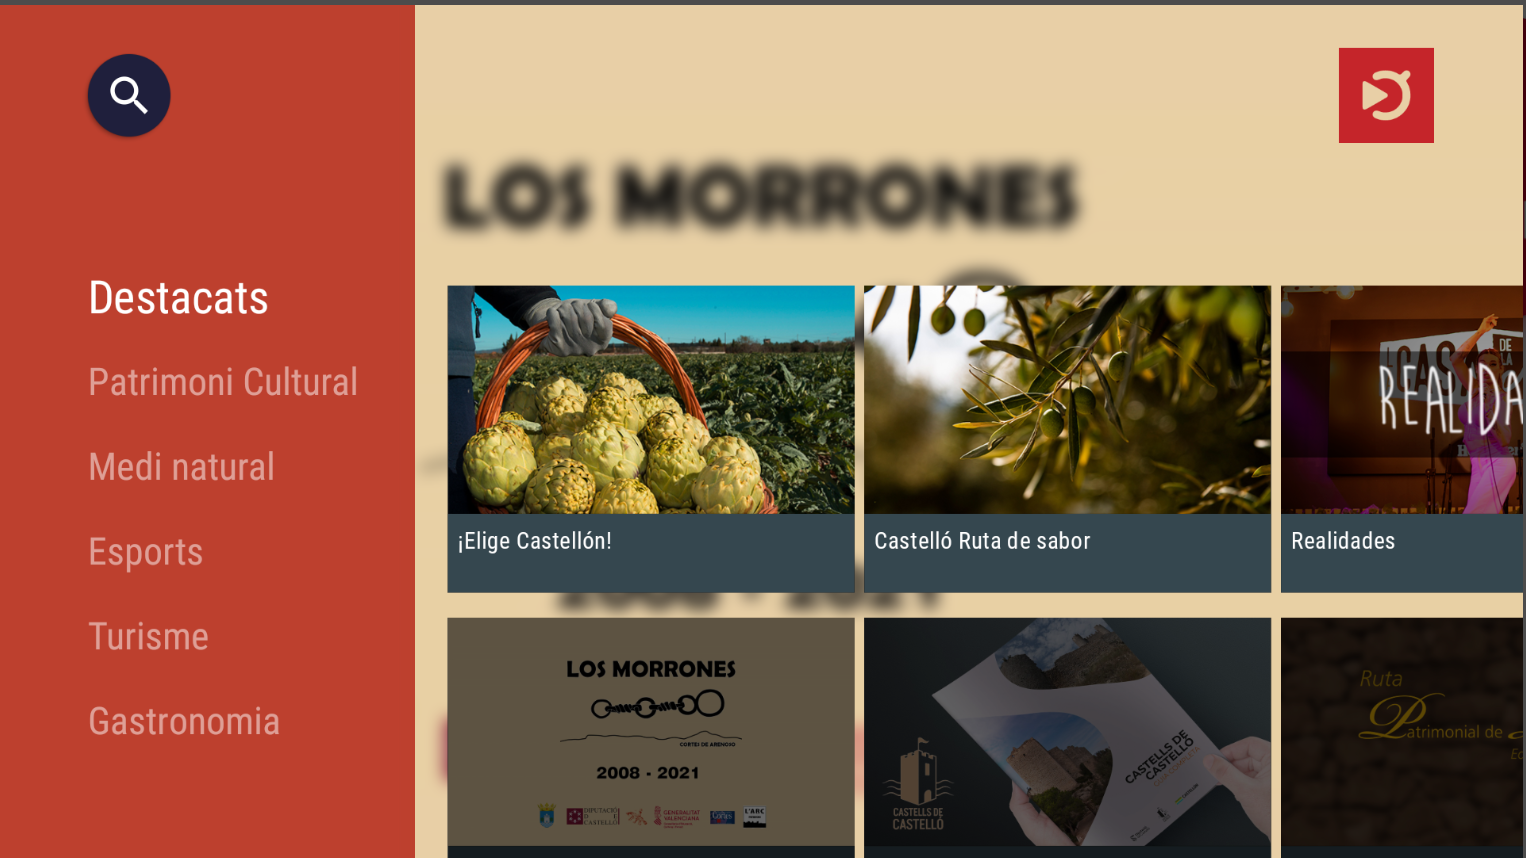
\includegraphics[width=0.8\textwidth]{imaxes/UX_inicios.png}
    \caption{Captura de la interfaz en las primeras fases del proyecto}
    \label{fig:UX_inicios}
\end{figure}
\begin{figure}[H]
    \centering
    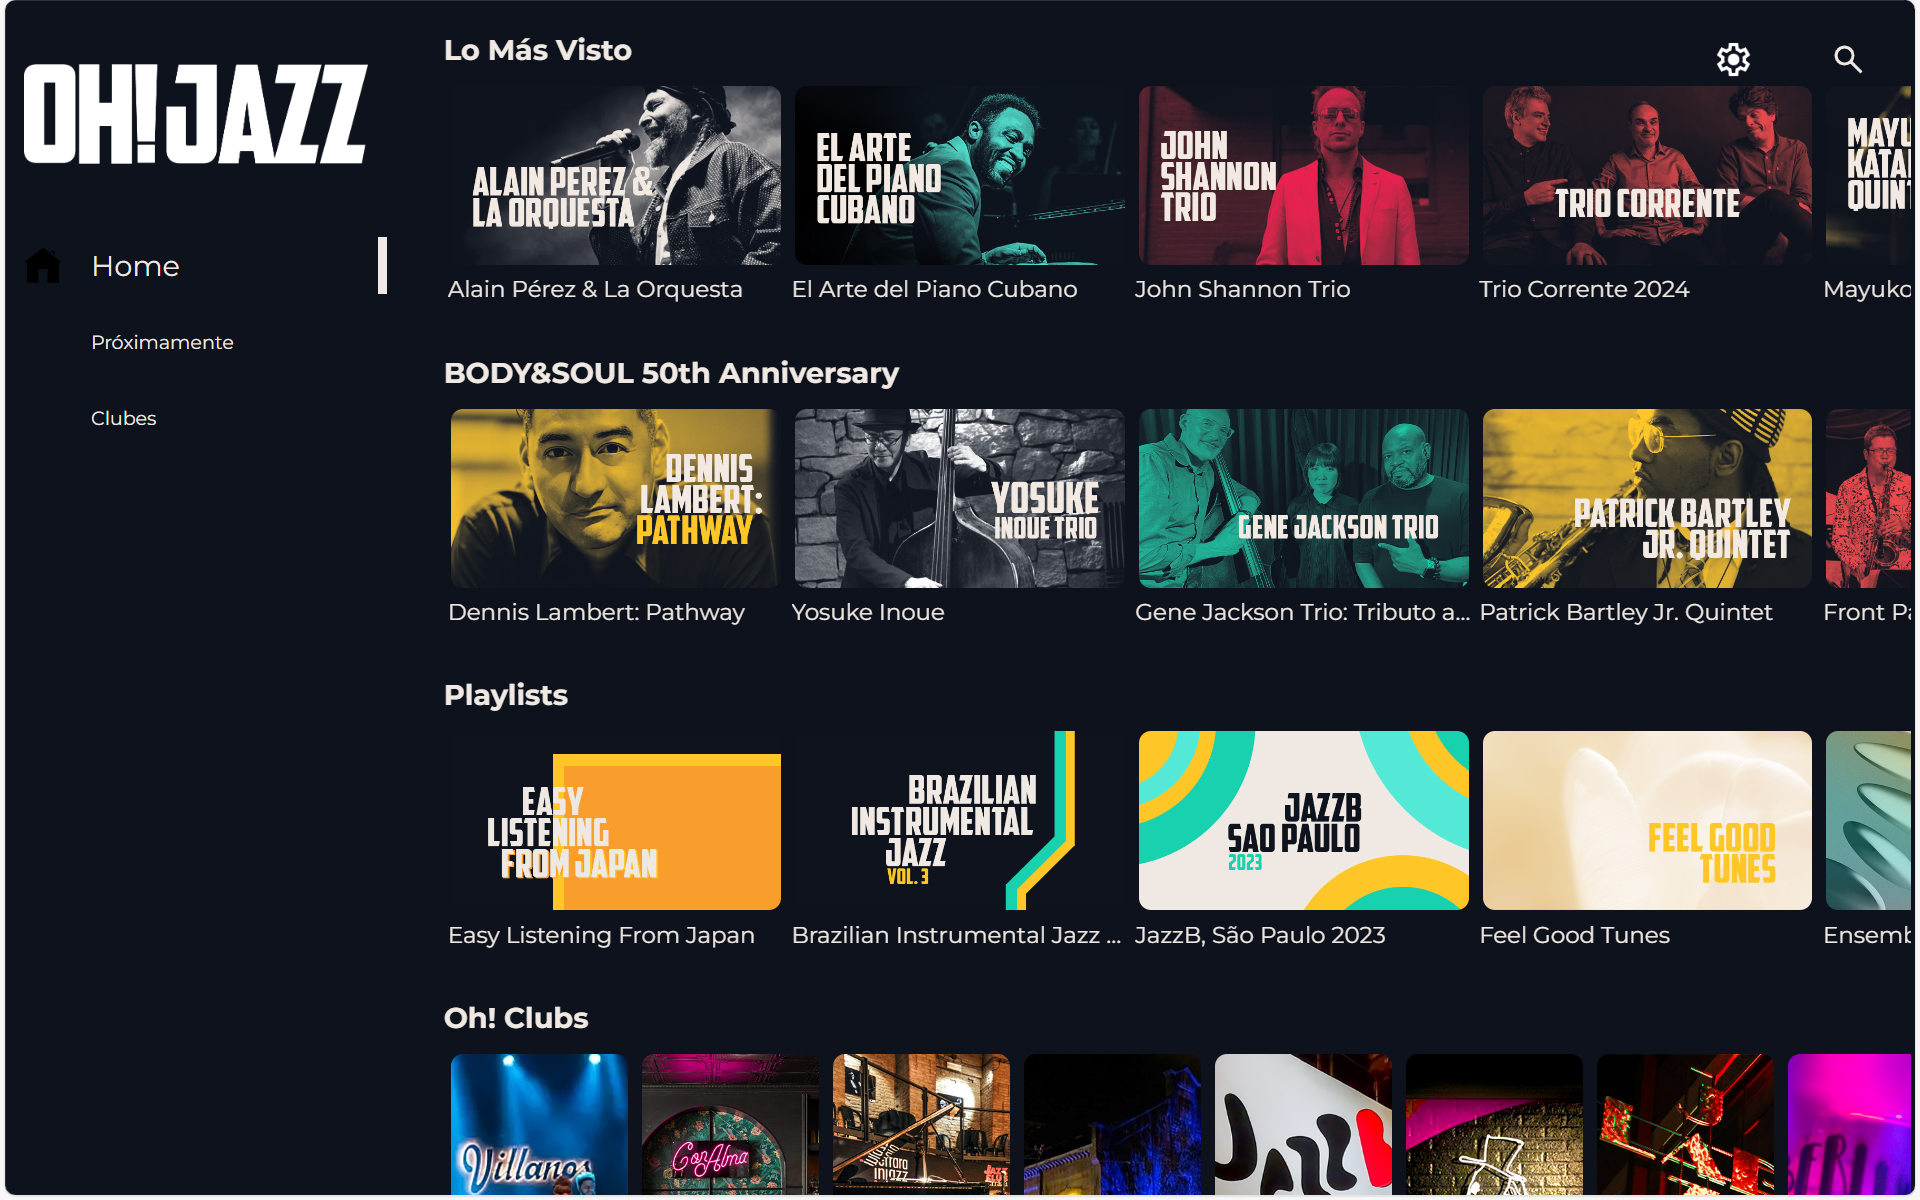
\includegraphics[width=0.8\textwidth]{imaxes/Home_desp_OhJazz.png}
    \caption{Captura de la interfaz más reciente, aún en pruebas por parte del cliente}
    \label{fig:Home_desp_OhJazz}
\end{figure}
\begin{figure}[H]
    \centering
    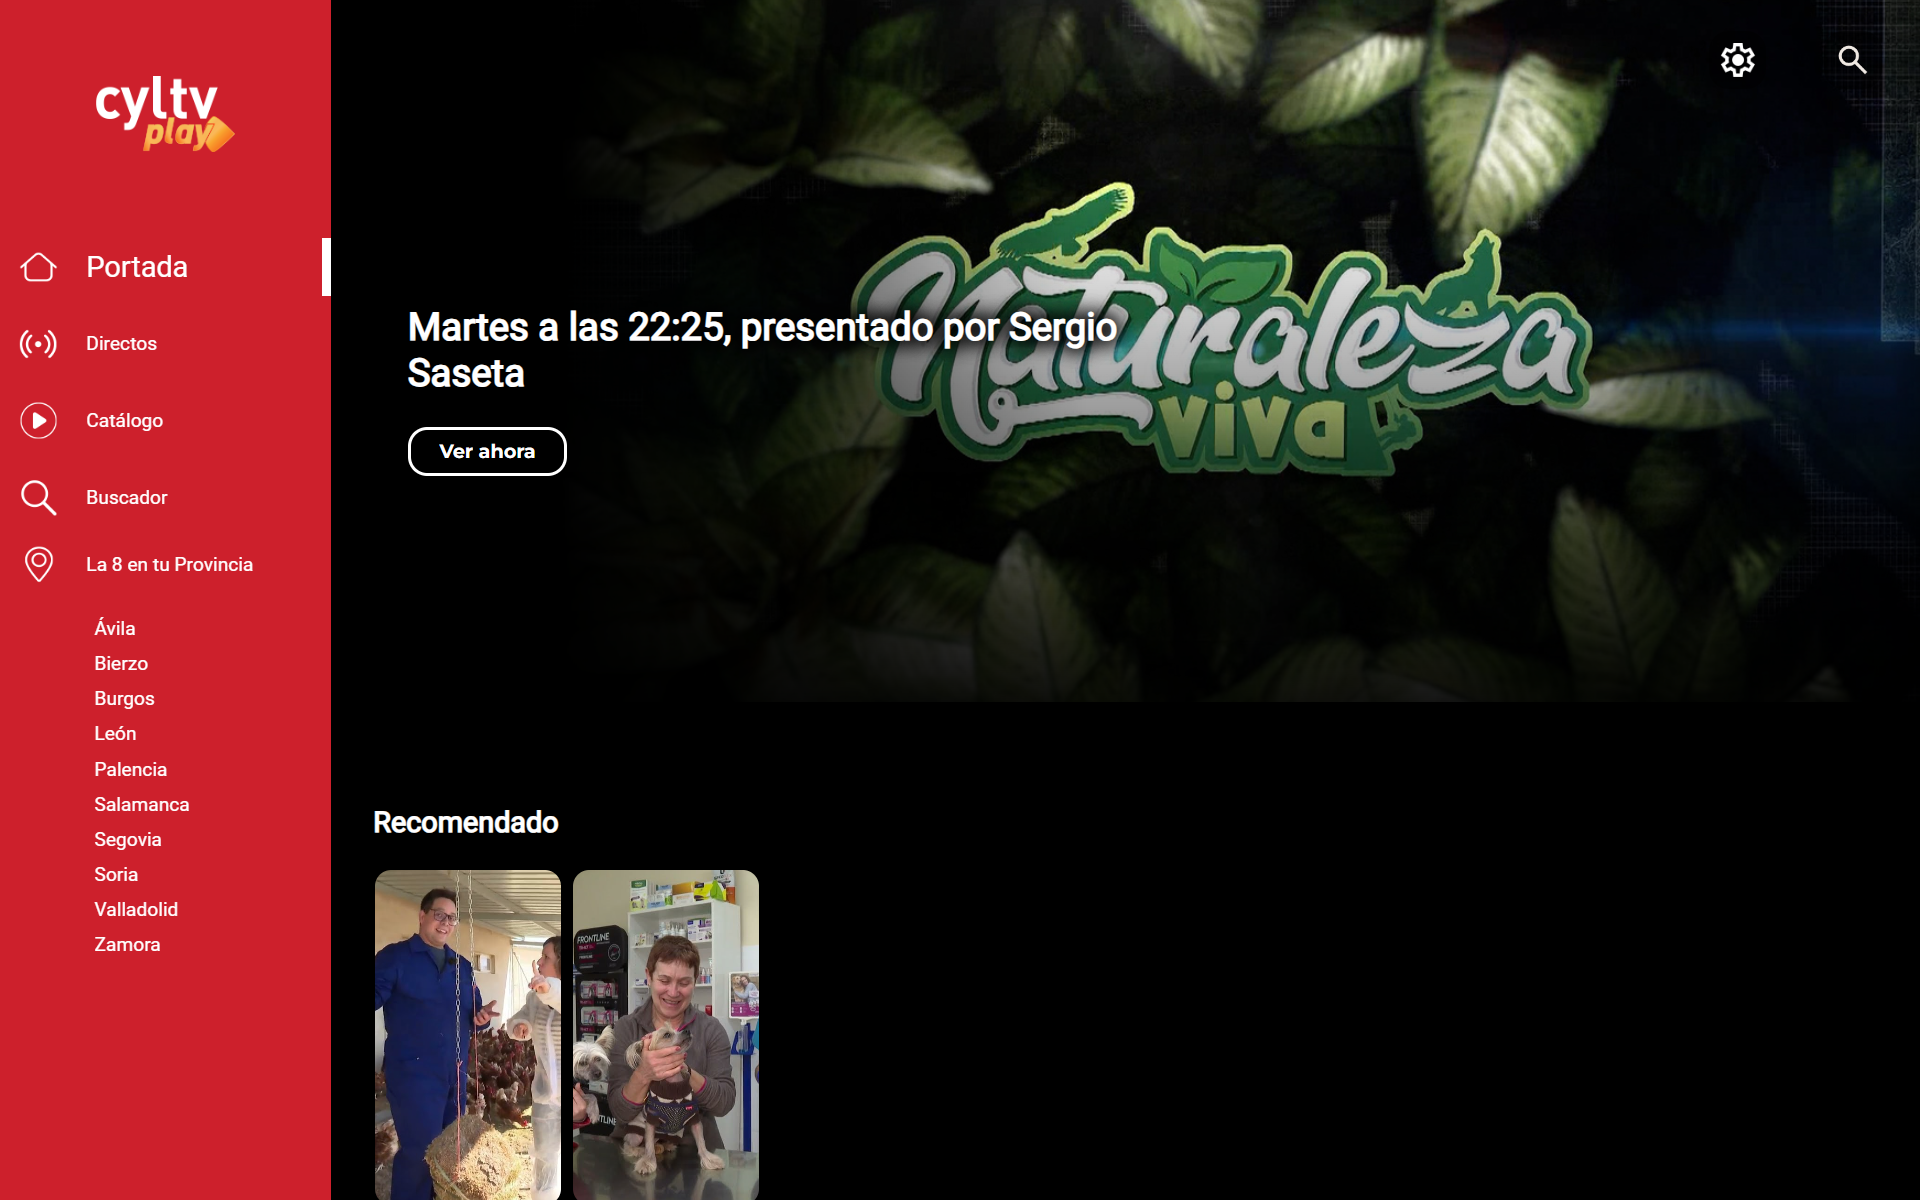
\includegraphics[width=0.8\textwidth]{imaxes/Home_CyLTv.png}
    \caption{Captura de la interfaz casi final}
    \label{fig:Home_CyLTv}
\end{figure}

Estas imágenes muestran la evolución de la interfaz de usuario de \textit{Ott}. La primera imagen refleja el diseño básico inicial, 
sin apenas funcionalidades. En la segunda, se observa un diseño más avanzado, aunque el cliente aún estaba ajustando parámetros (por ejemplo, 
la falta de visibilidad de los iconos de los menús o el contraste del fondo). Finalmente, la tercera imagen muestra la interfaz casi 
final, con un diseño pulido y todas las funcionalidades implementadas.

Más que enfocarse en un diseño único, el proyecto se ha centrado en el diseño de componentes y sus variantes. Algunos elementos de 
la interfaz tienen una estructura fija, aunque permiten personalizar colores y textos:

\begin{itemize}
    \item \textbf{Menú lateral:} Permite navegar por las secciones de la aplicación y se encuentra a la izquierda de la pantalla.
    \item \textbf{Menú superior:} Proporciona acceso a las opciones de configuración. Los iconos y colores de fondo son personalizables, pero la posición depende del número de opciones del menú.
    \item \textbf{Barra de búsqueda:} Situada en la pantalla de búsqueda, su posición y tamaño son fijos, pero utiliza los colores base del cliente para los efectos de foco y difuminado.
    \item \textbf{Lista de elementos:} Muestra los elementos disponibles en la aplicación. La estructura y tamaños son fijos, aunque el contenido y número de listas pueden personalizarse.
    \item \textbf{Detalle de elemento:} Muestra la información detallada de un elemento. Aunque la metadata y el contenido son personalizables, la estructura y disposición de los elementos son fijos. Se está trabajando para permitir mayor personalización desde el gestor de contenidos.
\end{itemize}

El cliente puede personalizar la interfaz ajustando colores de fondo, texto, botones, foco y añadiendo sus logos e imágenes, adaptando la 
aplicación a su identidad visual.
\subsubsection{Personalización de los componentes}
\label{sec:diseno-ux-personalizacion}

Como se ha mencionado anteriormente, el diseño de la interfaz de usuario se ha centrado en la creación de componentes y sus múltiples variantes. 
Estos componentes se dividen en dos tipos principales: \textit{contenidos} y \textit{contenedores}, cada uno de los cuales tiene un enfoque de 
diseño diferente dependiendo del tipo de \textit{widget} en el que se utilicen. Un \textit{widget} es un componente de la interfaz que almacena y 
muestra uno o varios contenidos de manera específica.

Cada tipo de \textit{widget} determina la presentación tanto de los contenidos como de los contenedores, lo que implica que se necesita un diseño y 
un código específico para asegurar que se muestren correctamente en la interfaz. A continuación, se detallan los aspectos clave que cambian según 
el tipo de \textit{widget}:

\begin{itemize}
    \item \textbf{Disposición de los contenidos:} Según el tipo de \textit{widget}, los contenidos se distribuyen de formas diversas. Si se trata de 
    un \textit{widget} de \textbf{destacados}, los contenidos se mostrarán con un tamaño más grande y ocuparán la parte superior de la pantalla, 
    siendo más llamativos. Estos \textit{widgets} pueden tener distintas configuraciones, como la inclusión de botones, un único contenido 
    destacado o varios en formato \textit{slider}, con opciones de distribución de texto e iconos. En contraste, un \textbf{mosaico} organizará los 
    contenidos de manera compacta en el centro de la pantalla. Para otros tipos de \textit{widgets}, como las listas horizontales, los contenidos 
    se dispondrán en filas secuenciales. Estos formatos son personalizables según las necesidades del cliente y el tipo de contenido que se desee resaltar.
    
    \item \textbf{Disposición de la información:} La cantidad y el tipo de información que se muestra también dependen del \textit{widget}. Por ejemplo, 
    en un \textbf{destacado}, el sistema puede mostrar el título, una descripción detallada y un botón de acceso al contenido. En un \textbf{banner}, 
    solo se mostrará el título del contenido. Esta flexibilidad en la información permite que los \textit{widgets} se ajusten a diferentes escenarios 
    y preferencias del cliente, lo que es clave para mantener una interfaz adaptable y eficaz.
    
    \item \textbf{Forma de las imágenes:} La forma y el tamaño de las imágenes asociadas a los contenidos varían según el tipo de \textit{widget}. 
    En los \textbf{destacados}, las imágenes suelen ser grandes, ocupando una buena parte de la pantalla, y pueden cambiar la distribución de la 
    información según el caso específico. En los \textbf{banners}, las imágenes tienen una orientación horizontal con un ratio de 16:9, mientras 
    que en los \textbf{posters}, las imágenes son verticales, con un ratio de 9:16. En los \textbf{posters}, las imágenes aparecen en un panel 
    lateral cuando el foco se mantiene en el contenido durante más de un segundo. Este enfoque garantiza una presentación visual coherente que 
    varía según el tipo de contenido y el diseño del \textit{widget}.
    
    \item \textbf{Otras características:} Algunos \textit{widgets} permiten funcionalidades adicionales que dependen del tipo de contenido que se esté 
    presentando. Por ejemplo, en los \textit{widgets} para contenidos en directo, puede aparecer una barra de progreso y el nombre del programa actual. 
    En un \textbf{widget banner-click}, diseñado para mostrar anuncios, se presenta un banner horizontal que ocupa casi todo el ancho de la pantalla, 
    y al hacer clic en él (excepto en televisores, donde esta opción está desactivada), redirige al usuario a una URL externa.
\end{itemize}

Estas personalizaciones, junto con otras más específicas o en desarrollo, deben estar correctamente implementadas y soportadas por la aplicación 
para garantizar que los \textit{widgets} seleccionados por el cliente funcionen sin problemas y no interfieran con el resto de la interfaz.

Adicionalmente, es importante tener en cuenta ciertas limitaciones en la personalización. Solo puede haber un \textit{widget destacado} por 
pantalla, los \textit{widgets} tipo \textbf{mosaico} con muchos elementos pueden sobrecargar la interfaz, y los \textbf{posters} se utilizan generalmente 
para destacar ciertos contenidos, mostrando información detallada sobre estos.

\subsubsection{Ejemplos de personalización}
\label{sec:diseno-ux-ejemplos}

A continuación se muestran algunos ejemplos de personalización de los widgets de la interfaz de usuario de \textit{Ott}.


\begin{figure}[H]
    \begin{subfigure}[c]{0.5\textwidth}
        
\includegraphics[width=\textwidth]{imaxes/Widget_banner.png}
        \subcaption{Ejemplo de un widget básico de tipo "banner"}
        \label{fig:Widget_banner}
    \end{subfigure}
    \hspace{0.1\textwidth}
    \begin{subfigure}[c]{0.5\textwidth}
        
\includegraphics[width=0.8\textwidth]{imaxes/Widget_destacado.png}
        \subcaption{Ejemplo de un widget básico de tipo "destacado"}
        \label{fig:Widget_destacado}
    \end{subfigure}
    \caption{Ejemplos de un widget básico de tipo "banner" y "destacado"}
    \label{fig:Widget_banner_destacado}
\end{figure}

\begin{figure}[H]
    \begin{subfigure}[c]{0.5\textwidth}
        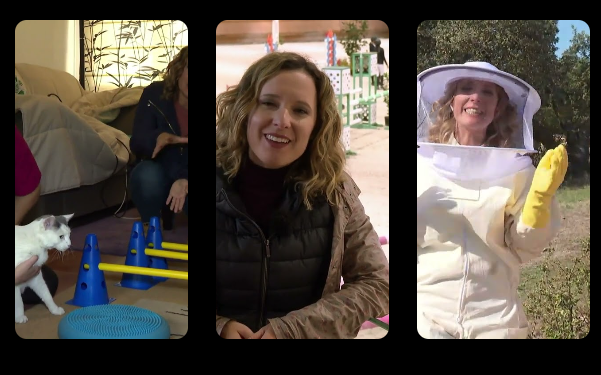
\includegraphics[width=\textwidth]{imaxes/Widget_poster.png}
        \subcaption{Ejemplo de un widget básico de tipo "poster"}
        \label{fig:Widget_poster}
    \end{subfigure}
    \hspace{0.1\textwidth}
    \begin{subfigure}[c]{0.5\textwidth}
        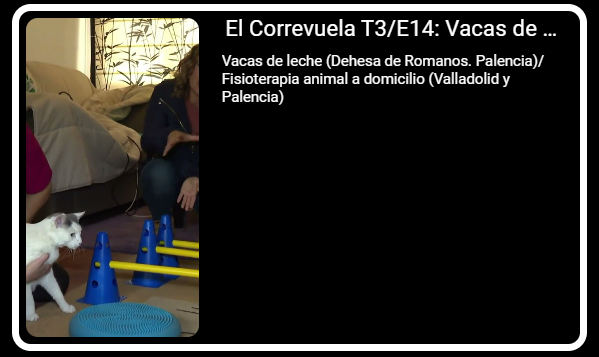
\includegraphics[width=\textwidth]{imaxes/Widget_poster_abierto.png}
        \subcaption{Ejemplo de un widget básico de tipo "poster" con la información mostrada}
        \label{fig:Widget_poster_abierto}
    \end{subfigure}
    \caption{Ejemplos de un widget básico de tipo "poster"}
    \label{fig:Widgets_poster}
\end{figure}


\subsection{Disgramas UML}
\subsection{Introducción}
\label{subsec:Analisis_introduccion}

Una vez completada una fase de análisis y claros los requisitos y objetivos del proyecto, vamos a trabajar sobre 
estos para definir las estructuras de datos, las funciones y los comportamientos del sistema. Se trata de una
fase previa a la implementación, en la que se definen los elementos que compondrán el sistema y cómo se relacionan
entre sí. 

En este apartado se describirá como fueron las primeras fases de diseño de las aplicaciones \textit{Ott} y \textit{Ott Data} 
y como se se trabaja en general en las fases de diseño de nuevas funcionalidades e iteracciones en el proyecto.


\subsection{Estudio y diseño de la aplicación de análisis de datos}
\label{sec:diseno-estudio}

\subsubsection{Diseño general}
\label{sec:diseno-general}

El diseño de la aplicación de análisis de datos se ha realizado siguiendo una metodología de diseño centrada en el usuario. 
Para ello, se ha realizado un análisis de las necesidades de los usuarios, se han definido los requisitos de la aplicación 
y se ha diseñado la interfaz de usuario.

Dentro de las necesidades de los usuarios y de los requisitos de la aplicación se destaca la necesidad de que la visualización
de los datos sea clara y sencilla y que para utilizar la aplicación no sea necesario tener conocimientos avanzados de análisis de datos.

En cuanto al diseño de la interfaz de usuario, se ha optado por un enfoque sencillo y minimalista, utilizando colores suaves y 
una tipografía clara y legible. La interfaz ha sido diseñada para ser intuitiva y fácil de usar, permitiendo al usuario acceder 
rápidamente a todas las funcionalidades de la aplicación. El diseño se centra en la visualización de gráficos y datos, presentando 
la información de manera ordenada y consistente, para que el usuario pueda comprenderla rápidamente. Todas las gráficas y tablas 
comparten un estilo uniforme y limpio, evitando elementos recargados que puedan distraer la atención.

De forma similar a la OTT, el diseño de la aplicacion de análisis de datos se ha realizado siguiendo un enfoque modular,
dividiendo la aplicación en diferentes componentes independientes que se comunican entre sí. Esto permite que la aplicación sea
más fácil de mantener y extender, ya que cada componente puede ser modificado o reemplazado sin afectar al resto de los componenetes 
ni a la interfaz. Además, el diseño modular facilita la reutilización de código y la integración de nuevas funcionalidades.

\subsubsection{Estudio de las agrupaciones de datos}
\label{sec:diseno-agrupaciones}

Una vez definidos los requisitos de la aplicación y el diseño general, era importante estudiar que agrupaciones de datos 
se podian lograr con las funcionalidades que ofrece Matomo y que opciones de visualización se podían implementar. 

Lo primero fue detectar que tipos de gráficos eran necesarios soportar y diseñar. Tras un análisis de la entrega de los datos
que hace Matomo se decidió comenzar con el soporte para gráficos lineales, de barras, circulares y tablas. Así, en función 
de la utilidad, periodo y enfoque de los datos, se podrán seleccionar diferentes tipos de gráficos para visualizar la información.

\paragraph{Páginas y secciones}
Lo siguiente era estudiar que páginas o apartados de la aplicación de análisis de datos se podían implementar. La primera página en la que 
se pensó fue la página de inicio o dashboard, en la que se mostrarán los gráficos que presenten una información más general y resumida
de los datos. 

Otra página en la que se pensó durante el análisis fue una página que permitiera al usuario comparar gráficas provenientes de diferentes
módulos. La idea era que el cliente tuviera la oportunidad de comparar varias gráficas de diferentes módulos en una misma página para 
poder analizar la información en busca de patrones, tendencias o correlaciones entre los datos.

El resto de páginas son dedicadas a agrupaciones de datos que tienen relación entre sí. La creación de estas páginas se enfocó en 
que fuera más dinámica y que permitiera la creación fácil y rápida de nuevas secciones. 



  \chapter{Implementación}
\label{sec:implementacion}

\input{contido/Implementacion/introduccion.tex}

\section{Implementación de la aplicación OTT}
\subsection{Desarrollo de la funcionalidades básicas}
\label{sec:desarrollo_funcionalidades_basicas}

En esta sección se va a desarrollar el proceso de implementación de las funcionalidades básicas de la aplicación OTT.
Como ya se indicó en anteriores puntos, las tecnologías utilizadas pra el desarrollo de la aplicación son JavaScript, HTML y CSS.

\subsubsection{Indicaciones previas}
\label{sec:indicaciones_previas}

Esta sección va a describir el comportamiento básico de la aplicación cuando está siendo utilizada en televisiones ya que
es el enfoque principal de la aplicación en estos momentos y es el enfoque que más desafios supuso durante el desarrollo del código.

Trabajar en aplicaciones para televisiones tiene una particularidad y es que hay diseñar la aplicación para ser utilizada
con un mando a distancia. Aunque en algunas televisiones existe la posibilidad de utilizar el "magic remote" que es un mando
a distancia que tiene un puntero que se mueve por la pantalla, la mayoría de las televisiones no tienen esta funcionalidad y
desarrollar la aplicacion únicamente para televisores con esta opción sería un error ya que limita mucho el mercado al que
se puede llegar. Es por eso que la aplicación esta desarrollada desde un punto de vista que permita ser utilizada con un mando
a distancia. Aun así, se ha tenido en cuenta la posibilidad de que la aplicación pueda ser utilizada con un puntero o un ratón
en el caso de los ordenadores ya que, aunque no fue un objetivo para las primeras versiones de la aplicación, uno de los objetivos del 
código es que sea transversal y pueda ser utilizado en cualquier dispositivo. 

\subsubsection{Creación de los componentes de la aplicación}
\label{sec:creacion_componentes_aplicacion}

El primer paso del desarrollo fue la creación de la estructura básica de la aplicación de los primeros componentes que se iban a utilizar y 
sobre los que se ejecutan las funcionalidades básicas de la aplicación. Estos componentes son los menús, los "widgets" y los contenidos.

La creación de estos componentes es una creación en cascada podriamos decir. Cuando se inicia la aplicación, se llama a través de la 
API de la empresa a lo que internamente conocemos como "interfaz". Esta interfaz es un JSON que contiene toda la información principal de la aplicación
y con la que se dan los primeros pasos de creación de la misma. En este JSON tendremos los colores utilizados a lo largo de toda la aplicacion (colores de fondo,
de los botones, de los textos, etc), las fuentes de texto, textos legales, imagenes (logos, splash, etc) y demás información que se utilizará para la personalización
para cada cliente de la aplicación. Dentro de esta información también se encuentra la información de los distintos menús que va a tener la aplicación. 

Para la creación de cada uno de estos menús existen dos opciones: que tengan una pantalla asignada o que sean menús con un comportamiento predefinido. Dentro de 
de los menús con comportamientos predefinidos encontramos los menús de configuración o perfil, de búsqueda y de catálogo. Estos casos tienen un comportamiento
específico y no necesitan la información sobre la pantalla que deben mostrar. 

\begin{itemize}
    \item \textbf{Configuración:} Este  menú alojará las distintas opciones de configuración que tenga cada aplicación. No siempre son las mismas, pero en función 
    de las características de la aplicación se mostrarán unas u otras. Si la aplicación para determinado cliente debe soportar multilenugaje, en este menú se podrá
    cambiar el idioma de la aplicación. Si la aplicación tiene usuarios registrados, se mostrará la información del usuario y se podrá cerrar sesión. Una funcionalidad
    que aparece en todas las aplicaciones es la de mostrar los términos y condiciones de la aplicación. Para otras funcionalidades hay que acordar con el cliente 
    pertinente los requisitos y se añadiria para su aplicación la funcionabilidad necesaria. 
    \item \textbf{Búsqueda:} Este menú alojará la funcionalidad de búsqueda de la aplicación. En este menú se podrá filtar todos los contenidos de la aplicación
    por el nombre del contenido.
    \item \textbf{Catálogo:} También conocido como "A la carta" permite mostrar en la misma página todos los contenidos disponibles para ver en la aplicación.
\end{itemize}

En el caso de los menús que tienen una pantalla asignada, esta pantalla contiene la lista de los "widgets" que se deben mostrar en ella. Estos widgets son contenedores
de elementos y cada uno en función de su tipo tendrá un diseño y unas funcionalidades asignadas. A su vez, para cada uno de estos widgets existirá una lista de los contenidos
junto con la información de cada uno de ellos. 

Por lo tanto, la creación de las pantallas principales se realiza de la siguiente manera:

\begin{itemize}
    \item Se consigue la información del menú a través de la API.
    \item Se analiza para saber si es un menú predefinido o si tiene una pantalla asignada. \begin{itemize}
        \item Si es un menú predefinido, se crea la pantalla según el comportamiento predefinido.
        \item Si tiene una pantalla asignada, se consigue la información de la pantalla. \begin{itemize}
            \item Se crea el elemento del DOM que contendrá la pantalla.
            \item A partir de la lista de widgets, se crea un elemento del DOM para cada uno de ellos.
            \item Se consigue la información de los contenidos de cada widget.
            \item Se crea cada uno de los contenidos con las características correspondientes en función del tipo del widget que los contiene.
            \item Se añade cada contenido al widget correspondiente según el orden correspondiente.
            \item Se añade el widget al elemento del DOM que contiene la pantalla.
        \end{itemize}
    \end{itemize}
\end{itemize}

A lo largo de la creación de cada elemento html se le irá asignando según el tipo de elemento y widget correspondiente una serie de clases que permitirán
darle el estilo gracias a las hojas de estilo CSS.

El tipo de widget también determina el comportamiento de los contenidos que contiene. Por ejemplo, si el widget es de tipo "featured" con el campo "slider" activado, 
los contenidos destacados se mostrarán en un carrusel. Si el widget es de tipo "mosaico" los contenidos se mostrarán en una cuadrícula y el movimiento en 
lugar de ser una lista que se mueve horizontalmente, será una cuadrícula que se mueve en ambas direcciones.

\subsubsection{Movimiento por la aplicación}
\label{sec:movimiento_aplicacion}

Una vez creados los elementos de la aplicación, el siguiente paso es poder movernos por ella. Para ello, se ha creado una serie de funciones que permiten
moverse por los distintos elementos de la aplicación. Para este punto se ha tenido en cuenta que la aplicación pueda ser utilizada con un mando a distancia
y por lo tanto, ese movimiento debe de estar desarrollado y controlado por el código. 

Cuando la aplicación se utiliza en televisión hay que tener en cuenta que se debe tener un foco en un elemento en todo momento. Este foco es el que indica
en qué elemento de la aplicación se encuentra el usuario y es el que permite moverse por la aplicación. Para esta aplicación, en las pantallas principales
se ha utilizado un foco fijo, es decir, por norma general el foco se encuentra siempre en la misma posición y son los elementos los que se mueven en función
de la dirección en la que se mueva el usuario hacia ese foco. 

El movimiento por los widgets se realiza de la siguiente manera:
\begin{itemize}
    \item \textbf{Movimiento horizontal:} El movimiento horizontal se realiza con las teclas de dirección izquierda y derecha. Si estamos en un widget, el movimiento
    se realizará en los contenidos del widget. Cada vez que se pulsa una tecla de dirección, el widget se mueve horizontalmente en función de la dirección en la que se 
    haya pulsado colocando el elemento seleccionado en la posición del foco.
    \item \textbf{Movimiento vertical:} El movimiento vertical se realiza con las teclas de dirección arriba y abajo. Si estamos en una pantalla y todavía quedan widgets
    por mostrar hacia la dirección en la que se ha pulsado, se desplazará la pantalla hacia arriba o hacia abajo en función de la dirección en la que se haya pulsado 
    hasta colocar el elemento seleccionado en la posición del foco.
    \item \textbf{Movimiento en carrusel:} En el caso de que el widget sea de tipo "featured" y tenga el campo "slider" activado, el movimiento se realizará en el carrusel
    de los contenidos destacados. En este caso, el movimiento horizontal cambiará la imagen y la información mostrada en el carrusel.
    \item \textbf{Movimiento en mosaico:} En el caso de que el widget sea de tipo "mosaico", el movimiento se realizará en la cuadrícula de los contenidos. En este caso
    los contenidos aparecen ordenados por filas de izquierda a derecha y de arriba a abajo. el movimiento vertical desplazará la pantalla hacia arriba o hacia abajo
    en función de la dirección en la que se haya pulsado y el movimiento horizontal en este caso en concreto sí que moverá el foco hacia el elemento seleccionado.
\end{itemize}

Por otro lado el movimiento por el menú lateral es más simple. Para acceder al menú lateral hay varias opciones: se puede acceder pulsando el boton "return" siempre y 
cuando estemos en una pantalla principal o se puede acceder pulsando la tecla "izquierda" siempre y cuando no queden más elementos a la izquierda. Una vez seleccionado
el menú este se despliega ocupando más sitio y muestra no solo los iconos si no también los nombres de los menús. Para moverse por el menú se utilizarán las teclas de 
arriba y abajo y el foco hará que el elemento seleccionado destaque en tamaño. 

\begin{figure}[H]
    \centering
    \begin{subfigure}[c]{0.1\textwidth} 
        
\includegraphics[width=\textwidth]{imaxes/OTT/menu_lateral_cerrado.png}
        \subcaption{Menú lateral colapsado}
        \label{fig:menu_lateral_cerrado}
    \end{subfigure}
    \hspace{0.05\textwidth}
    \begin{subfigure}[c]{0.1\textwidth}
        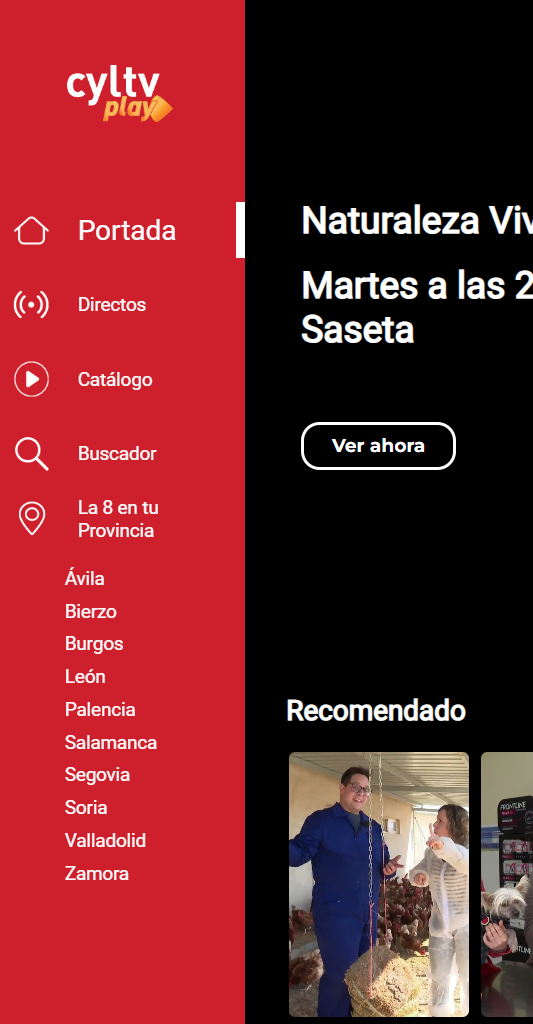
\includegraphics[width=\textwidth]{imaxes/OTT/menu_lateral_abierto.png}
        \subcaption{Menú lateral abierto}
        \label{fig:menu_lateral_abierto}
    \end{subfigure}
    \caption{Menú lateral}
\end{figure}

    
Durante el desarrollo del proyecto se han ido probando diferentes maneras de efectuar el movimiento. Se comenzó moviendo los 
elementos hacia el foco y más tarde se decició utilizar las funcionalidades de Html de "scroll", que permite mover elementos
sin realizar calculos de posición. Sin embargo, estas dos opciones fueron descartadas en favor de la utilización de 
las funcionalidades de "transform" de CSS. Tras analizar las tres opciones, la utilización de "transform" casi obligada. Si 
bien es cierto que la utilización de "scroll" es más sencillo y presenta multiples ventajas, su utilización es menos eficiente
y optima y por ello exige un mayor esfuerzo al navegador. En el caso de los ordenadores y dispositivo móviles este esfuerzo
no es tan significativo, pero en el caso de las televisiones, que tienen menos recursos, el esfuerzo es mucho mayor y la aplicación
se notaba lenta y pesada. La primera opción se descarto debido a que es mas efectivo y eficiente mover la pantalla con todos los elementos
que mover cada elemento por separado para reordenarlos.

En futuras implementaciones y con la aplicación mucho más optimizada no se descarta, de hecho se tiene en mente, la posibilidad de 
estudiar y volver a probar la funcionalidad de "scroll" debido a sus ventajas. Pero, por el momento, se seguirá utilizando la funcionalidad
de "transform" de CSS y no es un cambio urgente ni necesario ya que para el usuario de la aplicación no supone una diferencia significativa
en cuanto a funcionamiento, pero si en cuanto a rendimiento.


\subsubsection{Selección de un componente}
\label{sec:seleccion_componente}

Una vez que se ha movido el foco al elemento deseado, el siguiente paso es seleccionar ese elemento. Para ello, cada componenete tiene asociado un evento de selección
que se activa cuando se pulsa el botón de selección del mando a distancia. Este evento de selección es el que permite realizar la acción correspondiente al elemento
seleccionado. 

Estos eventos pueden ser creación de una nueva pantalla (en el caso de seleccionar una opción del menú lateral) o creación de una pantalla de detalle
(en el caso de seleccionar un contenido). En el caso de crear una nueva pantalla, se seguirá el mismo proceso que se ha seguido para la creación de la pantalla principal
y se mostrará la nueva pantalla en la aplicación, almacenando la pantalla anterior en una pila de pantallas. En el caso de seleccionar un contenido, se creará una pantalla
de detalle con la información del contenido seleccionado.

\subsubsection{Creación de la pantalla de detalle}
\label{sec:creacion_pantalla_detalle}

La pantalla de detalle es una pantalla que muestra la información detallada de un contenido. Esta pantalla se crea en función de la información que se 
recibe tras realizar una llamada a la API con el identificador del contenido seleccionado.

Existen dos tipos de pantallas de detalle en función del tipo del contenido: los contenedores y los contenidos. Los contenedores son aquellos contenidos que
contienen otros contenidos. Por ejemplo, una serie es un contenedor que contiene los capítulos de la serie. Los contenidos son elementos finales, como una película,
un capitulo, una partido, etc. Estos no tienen hijos asociados.

La pantalla de detalle de un contenedor está compuesta por una ficha con la información del elemento , una lista de los contenidos que contiene y una lista de los
contenedores relacionados. Para moverse por lo contenidos hijos haremos uso del movimiento vertical de igual forma que en la pantalla principal y una vez estemos 
en los contenidos relacionados el funcionamiento es el mismo que el de los widgets de la pantalla principal con el movimiento horizontal.

\begin{figure}[H]
    \begin{subfigure}[c]{0.5\textwidth}
        \includegraphics[width=\textwidth]{imaxes/OTT/pantalla_detalle_contenedor1.png}
        \subcaption{Pantalla de detalle de un contenedor}
        \label{fig:Widget_banner_contenedor}
    \end{subfigure}
    \hspace{0.1\textwidth}
    \begin{subfigure}[c]{0.5\textwidth}
        \includegraphics[width=\textwidth]{imaxes/OTT/pantalla_detalle_contenedor2.png}
        \subcaption{Pantalla de detalle de un contenedor}
        \label{fig:Widget_mosaico}
    \end{subfigure}
    \caption{Pantalla de detalle de un contenedor}
\end{figure}

Por otro lado, la pantalla de detalle de contenido está compuesta por una ficha con la información del contenido, donde se incluye el titulo, contenedor padre (si lo
tiene , en el caso de un capitulo de una serie, la serie a la que pertenece), una descripción corta, un botón que permite mostrar un popup con todo la información al 
completo, los iconos de rating y edad, un botón de reproducción y en caso de permitir la funcionalidad, un botón de añadir a favoritos. También tiene una lista de
contenidos relacionados.

\begin{figure}[H]
    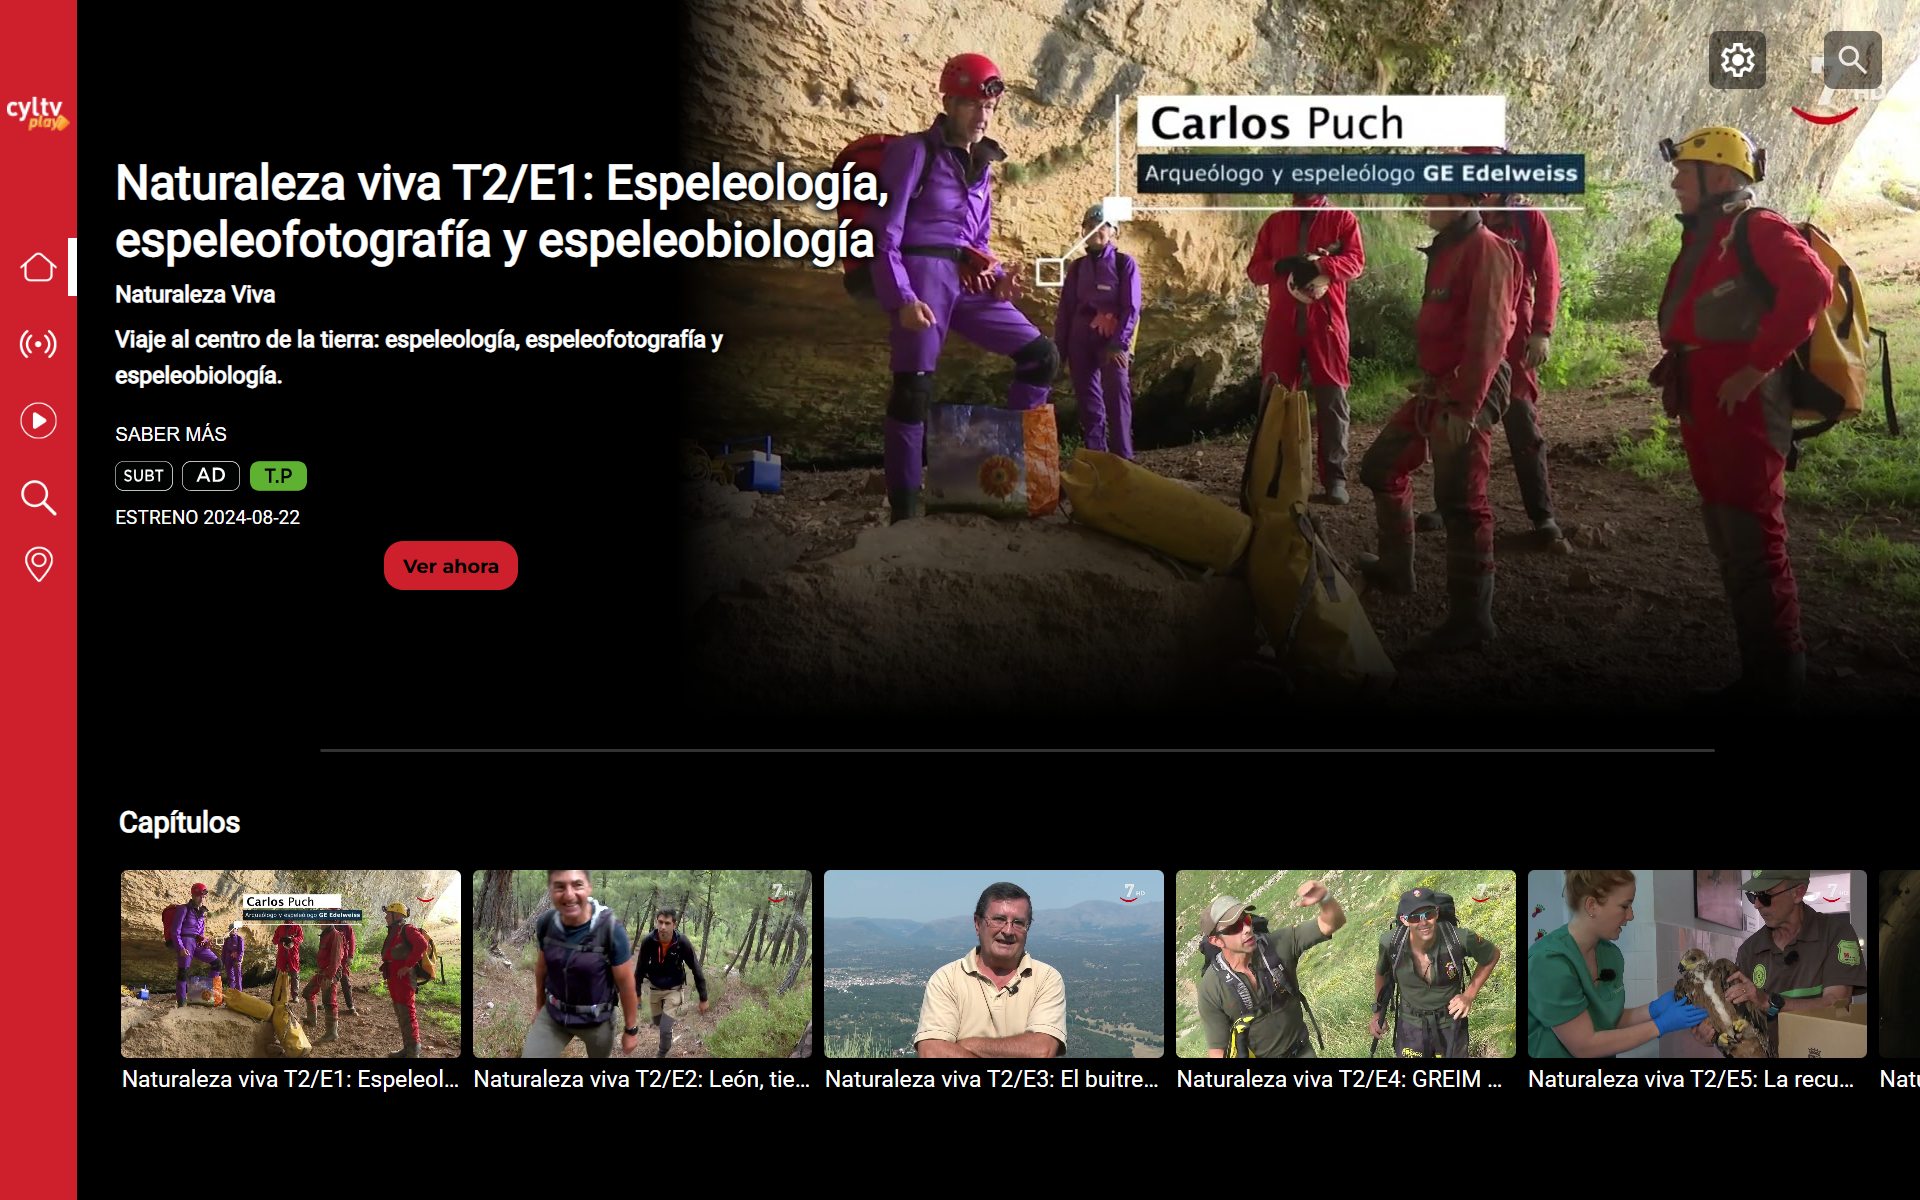
\includegraphics[width=0.4\textwidth]{imaxes/OTT/Pantalla_detalle_contenido.png}
    \caption{Pantalla de detalle}
\end{figure}

\subsubsection{Reproducción de un contenido}
\label{sec:reproduccion_contenido}

La reproducción de un contenido es una de las funcionalidades más importantes de la aplicación. Para acceder a ella hay dos opciones: a través de la pantalla de detalle
de contenido explicada en el punto anterior, o si un contenido tiene el trigger de reproducción activado, se podrá acceder a la reproducción directamente desde la pantalla
principal. Al seleccionar el botón de reproducción, la aplicación obtiene la información del contenido. En esta información se comprueba si el contenido 
necesita autentificación para ser reproducido y en caso afirmativo (el usuario ya deberia estar logueado) se comprueba si el usuario tiene permisos para ver el contenido.
Es una comprobación de seguridad ya que en caso de no tener acceso al contenido el botón de reproducción aparece como deshabilitado. En caso de tener acceso, el 
se realizan varias comprobaciones:

\paragraph{Origen del contenido:} Lo primero es comprobar de donde proviene el contenido. Aqui hay dos opciones: o esta alojado en la base de datos de la empresa o 
en la del cliente. Si esta en la del cliente la url del video estará ya en la información del contenido. En caso de estar en la base de datos de la empresa, hay que 
realizar una serie de comprobaciones para obtener la url del video. Estas comprobaciones son en base a si el contenido es gratuito o de pago ya que si es
gratuito la url se podra montar directamente con la información que se tiene, pero si es de pago hay que realizar una serie de comprobaciones para obtener la información.

\paragraph{Reproductor:} No todos los dispositivos pueden usar el mismo reproductor. Los ordenadores son más permisivos con este detalle, pero las televisiones no. En 
el caso de los ordenadores existe la opción incluso de que la API nos devuelva un player ya construido para utilizar directamente en la aplicación. Este caso no se utiliza
por el momento. Lo hace el código es detectar en que SO y con que contenido se esta trabajando. Aquí tenemos por el momento dos reproductores (VideoJs y ShakaPlayer) y dos 
tipos de video (VoD y Lives o Youtube). Para cada caso se monta el reproductor de una manera especifica. 

Una vez el video se está reproducciendo, el usuario dispone de las funcionalidades básicas para controlar la reproducción: pause, play, adelantar, retroceder y salir. 
En caso de permitir la funcionalidad y tener usuarios registrados la aplicación guarda el instante en el que se detuvo la reproducción para que el usuario pueda
continuar viendo el contenido en el mismo punto en el que lo dejó.

\subsubsection{Añadir a favoritos}
\label{sec:anadir_favoritos}

En caso de permitir usuarios registrados, la aplicación permite añadir a favoritos los contenidos. Para ello, en la pantalla de detalle de contenido se muestra un 
botón en forma de corazón que permite añadir el contenido a favoritos. En caso de que el contenido ya esté añadido a favoritos, el botón aparecerá en color rojo y pulsando
sobre él se eliminará de la lista de favoritos.

\subsubsection{Búsqueda de contenidos}
\label{sec:busqueda_contenidos}

La búsqueda de contenidos es una funcionalidad básica de la aplicación. Para acceder a ella se puede hacer de dos formas: a través del menú lateral o una opción 
situada en la parte superior derecha de todas las pantallas. Al abrir el menú de búsqueda, se muestra un campo de texto en el que se puede introducir el nombre del
contenido que se desea buscar. Una vez escrito el nombre completo o parcial del contenido y hacer click en el botón de búsqueda, la aplicación realiza una llamada a la
API con el nombre del contenido y obtiene una lista de los contenidos que coinciden con el nombre introducido. Esta lista se muestra en una pantalla de resultados de
búsqueda en forma de mosaico. 

\subsubsection{Obtención de la información de un directo}
\label{sec:obtencion_informacion_directo}

La obtención de la información de un directo es una funcionalidad que permite obtener la información de un directo en tiempo real. Para ello, la aplicación realiza una
llamada a la API con el identificador del directo y obtiene la información del directo en tiempo real a través de un epg. Este epg es un JSON que contiene la información
de los contenidos que se van a emitir en un periodo de tiempo determinado. La aplicación analiza este Json y obtiene la información del directo en tiempo real. De esta 
información se obtiene el titulo que se mostrará en el contenido correspondiente, y el progreso, que se calcula a partir de los tiempos de inicio y fin del contenido marcados
en el Json, y se muestra en la barra de progreso del contenido.


\subsection{Adaptación a los diferentes sistemas operativos de televisión}
\label{sec:adaptacion_introduccion}

El mercado de las televisiones inteligentes ha experimentado un gran crecimiento en los últimos años, lo que ha ampliado 
las opciones de aplicaciones y servicios disponibles para los usuarios. Sin embargo, este mercado es relativamente nuevo y 
se le exigen prestaciones similares a las de los dispositivos móviles u ordenadores personales. Cumplir con esas exigencias 
no es sencillo debido a varias razones: la capacidad de procesamiento de las televisiones, el soporte de los sistemas operativos 
a las tecnologías web y la diversidad de sistemas operativos disponibles.

\paragraph{Capacidad de procesamiento de las televisiones}
En los últimos años, la capacidad de procesamiento de las televisiones ha mejorado significativamente. Sin embargo, 
aún no es suficiente para ofrecer una experiencia de usuario comparable a la de un ordenador personal o un dispositivo móvil. 
Además, las tecnologías web son cada vez más complejas y exigentes, lo que hace que las televisiones no siempre puedan 
soportarlas. Al comparar la capacidad de procesamiento de una televisión de alta gama con la de un ordenador o un móvil, 
aunque las televisiones han mejorado, siguen estando por detrás de los dispositivos de consumo masivo en términos de rendimiento.

Las especificaciones de una televisión de alta gama actual (3-4 GB de RAM, procesador de 4 núcleos) son comparables a las de 
dispositivos móviles de gama media-alta de hace algunos años, que hoy en día ya cuentan con 6-8 GB de RAM y procesadores 
de 8 núcleos. De manera similar, los ordenadores más básicos ahora ofrecen entre 8 y 16 GB de RAM.

\paragraph{Soporte de los sistemas operativos a las tecnologías web}
Este problema está parcialmente relacionado con el anterior. Los sistemas operativos de las televisiones inteligentes no están 
tan adaptados a las tecnologías web como en otros dispositivos. Esto puede deberse tanto a la capacidad de procesamiento limitada 
como al hecho de que las televisiones entraron relativamente tarde en el mercado de los dispositivos inteligentes, lo que ha 
retrasado el desarrollo de aplicaciones y servicios optimizados para estos sistemas.

\paragraph{Diversidad de sistemas operativos}
Un problema adicional en el mercado de las televisiones inteligentes es la diversidad de sistemas operativos disponibles. Aunque en 
el mercado de los dispositivos móviles existen varios sistemas operativos, la mayoría de los móviles utiliza Android o iOS, lo que 
facilita el trabajo de los desarrolladores al crear aplicaciones. En cambio, la diversidad de sistemas operativos en las televisiones 
es mucho mayor, lo que obliga a los desarrolladores a adaptar sus aplicaciones a cada uno de ellos.

\subsubsection{Adaptación a los diferentes sistemas operativos de televisión}
\label{sec:adaptacion}

El mayor desafío de esta aplicación es su adaptación a los diferentes sistemas operativos de televisión. Desde las 
primeras fases, el objetivo principal ha sido asegurar su accesibilidad en televisores, dado que este era el 
objetivo a corto plazo. Sin embargo, siempre se tuvo en cuenta que debía ser una aplicación multiplataforma. 
Aunque la implementación y las pruebas han estado enfocadas en optimizar el rendimiento en televisores, la 
aplicación está diseñada para funcionar en ordenadores y dispositivos móviles. Reactivando ciertas funcionalidades, 
como el click o hover del ratón, la aplicación podría funcionar en web sin mayores problemas. No obstante, para 
dispositivos móviles, las pruebas han sido limitadas y aún se requieren nuevas adaptaciones, ya que su optimización 
es un objetivo a más largo plazo. Mientras tanto, la prioridad sigue siendo asegurar la consistencia en televisores, 
a medida que se prepara su lanzamiento en las tiendas de aplicaciones de los distintos sistemas operativos de televisión.

Adaptar una misma aplicación a partir del mismo código supone ajustarse a las capacidades y limitaciones de cada 
SO. Si un SO no soporta ciertas funcionalidades, lo ideal es buscar una alternativa que funcione en todos 
los dispositivos por igual, y en caso de no ser posible, se deberá buscar una solución específica para ese SO.

\subsubsection{Adaptaciones realizadas}
\label{sec:adaptaciones}

A continuación se detallan las adaptaciones generales realizadas para mantener la consistencia y el correcto
funcionamiento de la aplicación en los diferentes sistemas operativos de televisión.

\paragraph{Interfaz}
La interfaz debe ser consistente en cualquier dispositivo en el que se utilice la aplicación. Para ello, se ha 
utilizado un diseño "responsive" que se adapta a cualquier resolución de pantalla. Esto es necesario si queremos usarla 
en dispositivos de distintas familias, pero también en televisores de distintas marcas y modelos. Un ejemplo de ello son 
las televisiones utilizadas en este proyecto para pruebas: LG y Samsung, con la misma resolución de 1920x1080, y TCL (Android TV), 
con una resolución de 960x540. Aunque todas las televisiones son de gamas similares, las diferencias en resolución son evidentes, 
lo que hace esencial asegurarse de que la aplicación sea consistente en cualquier televisión disponible en el mercado. 

Para lograr esto, todo el diseño y las hojas de estilo CSS utilizan medidas relativas: porcentajes, "vh" y "vw". 
Se evita completamente el uso de medidas absolutas como "px", y también se evita el uso de "rem" y "em" para asegurar que 
el diseño sea coherente en todos los dispositivos.

\paragraph{Soporte de tecnologías web}
El soporte de tecnologías web es un aspecto crucial. Como se explicó en otras secciones, las tecnologías web utilizadas en 
este proyecto son JavaScript, HTML y CSS. Aunque todos los SO utilizados soportan estas tecnologías, no lo hacen completamente. 
Durante el desarrollo, se intentó minimizar el uso de librerías externas para garantizar la mantenibilidad del código y evitar 
problemas de compatibilidad en actualizaciones futuras. Un ejemplo de este desafío fue la eliminación de la funcionalidad 
de DOMParser, que no es compatible con Tizen, lo que obligó a implementar una solución manual para procesar archivos XML.

\paragraph{Navegación}
Un ejemplo de adaptación específica para cada SO es la navegación. Los comandos de los mandos a distancia varían ligeramente 
entre dispositivos, por lo que se creó una adaptación específica para cada uno. Cada SO cuenta con un archivo de configuración 
que traduce los códigos de los botones del mando a un formato común que la aplicación puede interpretar correctamente.

\paragraph{Reproducción de video}
La reproducción de video es una de las funcionalidades más importantes de la aplicación. En el caso de las televisiones inteligentes, 
las opciones de reproductores de video son más limitadas que en las páginas web. Por ejemplo, mientras que WebOS y AndroidTV 
soportan VideoJs, Tizen no, y en su lugar utiliza Shaka Player, que no es compatible con los otros SO. Para solucionar esto, 
la aplicación detecta el SO y ajusta el reproductor de video en consecuencia.

\paragraph{Detección del estado de la red}
La detección del estado de la red también varía entre sistemas operativos. Aunque se intentó unificar esta funcionalidad, 
no fue posible obtener resultados consistentes en todos los casos. En Tizen se utiliza la librería webApis, mientras que en 
AndroidTV y WebOS se emplea la funcionalidad "navigator.connection".

\paragraph{Cerrar la aplicación}
La forma de cerrar la aplicación varía entre sistemas. Se investigó la documentación de cada uno y se implementó 
la lógica necesaria para cerrar correctamente la aplicación según el SO detectado.

\subsubsection{Desafíos encontrados}
\label{sec:desafios}

Durante el desarrollo de la aplicación, surgieron varios desafíos que complicaron su adaptación. A continuación, 
se detallan algunos de los desafíos más importantes y las soluciones aplicadas.

El primer desafío fue la falta de información y soluciones para este tipo de aplicaciones. La mayoría de la información 
disponible proviene de la documentación oficial, que a menudo es limitada y no cubre todos los casos posibles. 
Los foros y comunidades de desarrolladores también son útiles, pero en muchos casos no ofrecen respuestas a 
problemas específicos en el desarrollo para televisores.

\paragraph{Foco automático en AndroidTV}
En las primeras pruebas en AndroidTV, se encontró un problema con el enfoque automático de los elementos en la pantalla. 
Esto provocaba movimientos inesperados en la interfaz al mover el mando. La solución fue desactivar este enfoque 
automático mediante un "listener" que interceptaba el evento de enfoque y lo desactivaba inmediatamente.

\paragraph{Botón de retorno con funcionamiento predefinido en AndroidTV}
Otro problema en AndroidTV fue el funcionamiento del botón de retorno. En la última actualización del SO, el botón 
cerraba automáticamente la aplicación si no había una página anterior en el historial. Como esta aplicación usa 
un diseño de página única, se interceptó el evento de retorno y se anuló su comportamiento predeterminado.

\paragraph{Splash screen en AndroidTV}
Finalmente, se encontró un problema con el "splash screen" predeterminado de Cordova en AndroidTV, que no se podía 
desactivar. Aunque se logró cambiar la imagen mostrada, el formato aún presenta problemas. Se sigue buscando una 
solución definitiva para este problema.


\section{Implementación de la aplicación de análisis de datos}
\subsection{Instalación, configuración e integración de la API de Matomo}
\label{sec:configuracion-matomo}

Para la construcción y desarrollo de la aplicación de análisis de datos, se ha utilizado la herramienta de análisis web Matomo. 
Aunque existen otras herramientas de análisis web, como Google Analytics, para un primer desarrollo se ha optado únicamente por 
esta herramienta, ya que es la más utilizada en las distintas aplicaciones de la empresa. 

Matomo \cite{matomo} es una herramienta de análisis web de código abierto que permite a los administradores de sitios web
obtener información sobre los visitantes de sus aplicaciones y páginas web. Ofrece una amplia gama de funcionalidades, como la
recopilación de datos, la generación de informes y la personalización de los mismos. Una de las funcionalidades que ofrece es 
la utilización de una API REST, que permite a los desarrolladores acceder a los datos recopiados por Matomo y realizar operaciones
sobre ellos. 

Con estas consultas, se puede obtener la información necesaria para la construcción de la aplicación de análisis de datos.
A través de la API se obtienen los datos que que servirán como entrada para la construcción de las gráficas y tablas.

Matomo ofrece una rápida y sencilla instalación e integración con las distintas aplicaciones en las que se requiera la 
recogida de datos. Los pasos a seguir son: 

\begin{enumerate}
    \item Darse de alta en la plataforma de Matomo.
    \item Dar de alta un nuevo sitio web en la plataforma.
    \item Descargar el código de seguimiento y añadirlo a la aplicación.
\end{enumerate}

Con estos pasos, Matomo comenzará a recopilar los datos de los visitantes de la aplicación. Si se desea obtener información más
detallada y concreta existen más opciones de configuración, como la creación de eventos personalizados, la configuración de
objetivos o la creación de segmentos. Para conocer datos sobre las reproducciones de los vídeos, habrá que configurar el reproductor
de vídeo para que envíe eventos a Matomo cada vez que se reproduzca un vídeo.

\paragraph{Ejemplo de código de seguimiento de Matomo}

\begin{lstlisting}[language=HTML]
    <!-- Matomo -->
    <script>
    var _paq = window._paq = window._paq || [];
    /* tracker methods like "setCustomDimension" should be called before "trackPageView" */
    _paq.push(['trackPageView']);
    _paq.push(['enableLinkTracking']);
    (function() {
        var u="https://tiivii-ott.matomo.cloud/";
        _paq.push(['setTrackerUrl', u+'matomo.php']);
        _paq.push(['setSiteId', 'IdSite']);
        var d=document, g=d.createElement('script'), s=d.getElementsByTagName('script')[0];
        g.async=true; g.src='https://cdn.matomo.cloud/tiivii-ott.matomo.cloud/matomo.js'; s.parentNode.insertBefore(g,s);
    })();
    </script>
    <!-- End Matomo Code -->
\end{lstlisting}

Una vez Matomo ya está recopilando los datos, se puede comenzar a realizar consultas a la API para obtener la información
necesaria. Para ello, se debe obtener un token de acceso a la API disponible en la configuración de la cuenta de Matomo y 
registrar la URL de la página web en la que se está realizando la consulta. Con esta configuración lista, y conociendo los
datos que se quieren obtener \ref{sec:diseno-estudio} y a través de qué métodos, se puede comenzar a realizar las consultas 
a la API. 

\subsection{Desarrollo de la aplicación de análisis de datos}
\label{sec:desarrollo-matomo}

Una vez configurada la API de Matomo, se puede comenzar a realizar consultas a la misma para obtener la información. Esta información
será la que se utilizará para la construcción de las gráficas y tablas que se mostrarán en la aplicación de análisis de datos.

Para la obtención, procesamiento y gestión de los datos, se ha desarrollado la aplicación con un enfoque escalable y mantenible.
Durante el desarrollo se ha utilizado la tecnología de React, una biblioteca de JavaScript para la creación de interfaces de usuario.
 Complementado con el uso de Html y Css y diversas librerías y APIs. 

\subsubsection{Estructura de la aplicación}
\label{sec:estructura-aplicacion}

La aplicación está compuesta por varios módulos cada uno encargado de una tarea específica. La estructura de la aplicación es la
siguiente:

\begin{itemize}
    \item \textbf{Configuración:} Módulo encargado de la configuración de la aplicación. Gracias a este módulo la aplicación
    crea las URLs necesarias y realiza las consultas a la API de Matomo. Cada URL está formada en función del módulo 
    correspondiente de Matomo, la acción pertinente y las variables necesarias para la consulta. También existen configuraciones
    para indicar que gráficos y datos se muestran en cada página. 
    \item \textbf{Consultas:} Módulo encargado de realizar las consultas a la API de Matomo. En este módulo se encuentran las
    funciones que realizan las consultas a la API y devuelven los datos obtenidos. Para cada acción se intenta llamar al Módulo
    API y a la acción getProcessedReport para obtener toda la información que nos ofrece Matomo acerca de cada acción. 
    \item \textbf{Procesamiento:} Módulo encargado de pedir y procesar los datos obtenidos para crear las distintas páginas
    de la aplicación. Para cada página se buscarán los datos y llamadas asignadas para la creación de la página, se pedirán 
    los datos y se enviarán a los componentes de gráficas y tablas para su creación y ordenará los resultados de estos componentes 
    para mostrarlos en la página.
    \item \textbf{Componentes:} Dentro de este módulo se encuentran los componentes de gráficas y tablas que se utilizan en la
    aplicación. Cada componente es un archivo independiente que se encarga de la creación de una gráfica o tabla en concreto.
    \item \textbf{Diseño:} En este módulo se encuentran las hojas de estilo de Css que se utilizan en la aplicación para darle
    un diseño más atractivo y usable.
\end{itemize}

\subsubsection{Desarrollo de la aplicación}
\label{sec:desarrollo-aplicacion}

Para el desarrollo de la aplicación haciendo uso de la API el primer paso tras tener configurado y listo Matomo fue obtener un 
servidor donde alojar la aplicación ya que por seguridad el API bloquea las consultas que se realizan desde un servidor local.
Para ello se utilizó el servicio de Netlify \cite{netlify}, un servicio de alojamiento de aplicaciones web que permite desplegar aplicaciones
de forma sencilla y rápida.
   
Una vez alojada la aplicación, se comenzó a desarrollar la aplicación. Para ello se se comenzó con los archivos de configuración
los cuales se encargan de crear las URLs necesarias para realizar las consultas a la API. 

\paragraph{Ejemplo de archivo de configuración de la API de Matomo}
\begin{lstlisting}[language=Java]
    const methodBase = 'MediaAnalytics';
    const module = 'API';

    export const MediaAnalytics_get = (idSite, period = 'day', date = '2023-12-01,2024-07-01') => {
        const method = `${methodBase}.get`;
        return { url: getBaseUrl(module ,method, { idSite, period, date }), title: 'Overall Metrics' };
    };

    export const MediaAnalytics_getCurrentNumPlays = async (idSite, lastMinutes = 180) => {
        const action = 'getCurrentNumPlays';
        const method = `${methodBase}.getCurrentNumPlays`;
        return await fetchData(idSite, { module: methodBase, action,url: getBaseUrl(module ,method, { idSite, lastMinutes })});
    };

\end{lstlisting}

Estos archivos reciben los parámetros necesarios para realizar las consultas a la API, crean la URL (getBaseUrl) y consiguen los
datos (fetchData) necesarios para la creación de las gráficas y tablas. 

\paragraph{Función para la creación de la URL de la API de Matomo}
\begin{lstlisting}[language=Java]
    export const getBaseUrl = (module, method, params = {}) => {
        const baseUrl = `${baseURL}index.php?module=${module}&format=${format}&method=${method}&token_auth=${token_auth}`;
        const queryParams = new URLSearchParams(params).toString();
        return `${baseUrl}&${queryParams}`;
  };
\end{lstlisting}

\paragraph{Función para la obtención de los datos de la API de Matomo}
\begin{lstlisting}[language=Java]
    
export const fetchData = async (idSite, requestData) => {
    var newChartData = null;
    try {
      try {
        let dataUrl = API_getProcessedReport(idSite, 'year', 'yesterday', requestData.module, requestData.action, language);
        let response = await axios.get(dataUrl.url);
        var processedData = response.data;
      } catch (error) {
        console.error('Error fetching data:', error);
      }
  
      // Usar la función de API general
      const response1 = await axios.get(requestData.url);
      const responseData = response1.data;
  
      const data = {
        value: responseData,
        info: processedData ? processedData : {}
      };
  
      newChartData = data;
      console.log('Data fetched:', newChartData);
    } catch (error) {
      console.error('Error fetching data:', error);
    }
  
    return newChartData;
  };
\end{lstlisting}


Una vez obtenidos los datos, a través de la configuración de la página pertinente y con el formato adecuado y unificado se envían
a los componentes de gráficas y tablas para su creación. Una vez creados los componentes, estos son añadidos a la página y se
muestran los resultados.

\paragraph{Ejemplo de creación de una gráfica}
\begin{lstlisting}[language=Java]
    return (
        <div key={index} className="data-table-section">
          <h2>{chartConfig.title}</h2>
          <div className="chart-group">
            {metrics.map((metric, metricIndex) => (
              <GraphRenderer
                key={metricIndex}
                chart={{
                  type: chartConfig.type,
                  labels: labels,
                  data: dataPoints[metric],
                  title: chartConfig.metrics[metric],
                  metricType: chartConfig.data.info?.metadata.metricTypes[metric] || 'number',
                }}
              />
            ))}
          </div>
        </div>
      );
\end{lstlisting}

Para detectar los formatos y los componentes que hay que crear, se creo el componente GraphRenderer que recibe los datos y el
tipo de gráfica que se quiere crear y se encarga de llamar al componente correspondiente para la creación de la gráfica. Este componente
se creo como puentre entre los datos y los componentes de gráficas y tablas para favorecer la escalabilidad y mantenibilidad de la
aplicación. 

\paragraph{Código del componente GraphRenderer}
\begin{lstlisting}[language=Java]
    
    const GraphRenderer = ({ chart, chartIndex }) => {
        const { type, labels, data, title, metricType } = chart;
    
    
        switch (type) {
        case 'lineal':
            return (
            <div className="graph_component" key={chartIndex}>
                <ChartComponent
                labels={labels}
                data={data}
                label={title}
                title={title}
                metricType={metricType}
                />
            </div>
            );
    
        case 'pie':
            return (
            <div className="graph_component" key={chartIndex}>
                <PieChartComponent
                labels={labels}
                data={data}
                title={title}
                />
            </div>
            );
            ...
        }
    };
\end{lstlisting}


Para la creación de los distintos gráficos y tablas se han utilizado la librería de Chart.js \cite{ChartJS}. Esta librería
permite la creación de gráficos y tablas de forma sencilla y rápida. Ofrece una amplia gama de gráficos y tablas que se pueden
personalizar y adaptar a las necesidades de la aplicación. Es muy flexible lo que permite la creación de gráficos y tablas
adaptado a las necesidades de la aplicación. Se han utilizado los componentes Line, Bar, Pie y Bubble por el momento para 
la creación de las gráficas.

\paragraph{Ejemplo de creación de un grafico lineal}
\begin{lstlisting}[language=Java]
    
const ChartComponent = ({ data, labels, title, metricType }) => {
    const chartData = {
      labels,
      datasets: [
        {
          label: title,
          data,
          fill: false,
          backgroundColor: 'rgba(75, 192, 192, 0.6)',
          borderColor: 'rgba(75, 192, 192, 1)',
        },
      ],
    };
  
    if(metricType === 'percentage') {
      chartData.datasets[0].yAxisID = 'percentage';
    }
    const options = {
      scales: {
        x: {
          beginAtZero: true,
        },
        y: {
          beginAtZero: true,
        },
      },
    };
  
    return (
      <div className="graph">
        <h2>{title}</h2>
        <Line data={chartData} options={options} />
      </div>
    );
  };
\end{lstlisting}

Como se puede ver en el ejemplo de código, ChartJs permite la personalización de los distintos componente modificando los colores, 
títulos, ejes, etc. 

\subsubsection{Automatización y configuración de las páginas}
\label{sec:automatizacion-configuracion-paginas}

Siguiendo con el enfoque de escalabilidad y mantenibilidad de la aplicación, las aplicaciones se han creado de forma dinámica.
Para cada página existe un archivo de configuración que indica que metodos y acciones se deben realizar para la creación de la
página. Existe otro archivo con la información básica de cada gráfica por si la llamada a API.getProcessedReport no devuelve la
información necesaria y con la función para obtener los datos correspondiente para crear dicha gráfica. 

\paragraph{Ejemplo de archivo de configuración de una página}

\begin{lstlisting}[language=Java]
    export const pagesConfig = [
  {
    path: '/visitorSummary',
    title: 'Resumen del visitante',
    chartsConfig:visitCharts_summary,
    components: ["chartOptions", "DataOverviewTable", "GraphRenderer"],
  },
  {
    path: '/visitTime',
    title: 'Tiempo',
    chartsConfig: visitCharts_time,
    components: ["GraphRenderer", "periodSelecter"]
  },
  ...
];
\end{lstlisting}

\paragraph{Ejemplo de archivo de configuración de una gráfica}

\begin{lstlisting}[language=Java]
    export const visitsCharts_frequency = [
    {
      title: 'Visits - Frequency',
      description: 'Get the frequency of visits.',
      action: "get",
      module: 'Visits',
      period: 'month',
      date: '2024-03-01,yesterday',
      type: 'lineal',
      metrics: {
        "nb_visits_new" : "Nuevas visitas",
        "nb_visits_returning": "Visitas que regresan"
      },
      data : [],
      params: ["period"],
      fetchDataFunction: visitFrequency_get,
      async getData(idSite, period = this.period, date = this.date){
        this.data = await visitFrequency_get(idSite, period, date)
        if(this.data.info.metadata){
          this.description = this.data.info.metadata.documentation;
          this.title = this.data.info.metadata.name;
          this.metrics = this.data.info.columns || this.data.info.metadata.metrics || this.metrics;
        }  
        return this;
      }
      
    },
   
  ];
\end{lstlisting}

Esta función se llamará desde la página correspondiente y se comenzará el proceso de creación de las gráficas. 

\subsubsection{Context y Hooks}
\label{sec:context-hooks}

Para la gestión de los datos y la comunicación entre los distintos componentes de la aplicación se ha utilizado la API de Context
y Hooks de React. Context es una API que permite compartir datos entre componentes de la aplicación sin tener que pasar los datos
a través de props. Se crea un contexto y se envuelve la aplicación en un componente que provee el contexto. Los componentes utilizarán
el contexto para acceder a los datos. 

En el caso de esta aplicación, se ha creado un contexto para la detección del id del sitio web que se está analizando. Este id
se utiliza para realizar las consultas a la API de Matomo y obtener los datos correspondientes a ese sitio web. 

\paragraph{Ejemplo de uso de Context:}   
\begin{verbatim}
    const { idSite } = useContext(IdSiteContext);
\end{verbatim}

Hooks es una API que permite a los componentes de la aplicación utilizar el estado y otras características de React sin tener que
escribir una clase. Se utilizan para la gestión del estado de los componentes y para la comunicación entre los distintos componentes
de la aplicación. 

Los hooks más utilizados en la aplicación son useState y useEffect (y useContext para el uso de Context del id). 

\paragraph{UseState: } Hook que permite añadir estado a los componentes funcionales y actualizarlo cuando sea necesario.

\begin{verbatim}
    const [isLoading, setIsLoading] = useState(true);
\end{verbatim}

\paragraph{UseEffect: } Hook que permite realizar efectos secundarios en los componentes funcionales. Se ejecuta después de cada
renderizado del componente.

\paragraph{Ejemplo de uso de useEffect para la actualización de los datos cuando cambia el id del sitio web:}
\begin{verbatim}
    useEffect(() => {
        const fetchData = async () => {
          setLoading(true);
          try {
            const evolutionData = await homeCharts_VisitsSection_Evolution.getData(idSite); 
            setVisitsEvolution(evolutionData);
          } catch (error) {
            console.error('Error fetching visits data:', error);
          } finally {
            setLoading(false);
          }
        };
        fetchData();
      }, [idSite]);
\end{verbatim}


\subsubsection{Despliegue de la aplicación}
\label{sec:despliegue-aplicacion}

Conforme se iba desarrollando la aplicación, se iban realizando pruebas para comprobar que todo funcionaba correctamente.
Para realizar estas pruebas se utilizó postman, una herramienta que permite realizar peticiones a una API y comprobar que los
datos devueltos son los correctos y el servicio de Netlify \cite{netlify} que permite desplegar aplicaciones de forma sencilla y rápida
para comprobar que la aplicación se desplegaba correctamente. Por el momento la aplicación sigue alojada en Netlify y se puede
acceder a ella a través de la URL \url{https://kanaloa-dev.netlify.app}
\subsection{APIs y librerías utilizadas}
\label{sec:apis-librerias}

\subsubsection{Librerias}
\label{sec:librerias}

Para la implementación de la aplicación de análisis de datos se han utilizado diversas librerías que facilitaron el desarrollo de la misma.
Estas librerías establecen una serie de funciones y métodos que permiten realizar operaciones de forma más sencilla y rápida que si se
tuviesen que implementar desde cero. 

Una de estas librerías es \textit{Axios}. Esta librería facilita la realización de peticiones HTTP desde el cliente a un servidor.
Esta popular herramienta está basada en promesas que simplifica la comunicación con APIs. Permite realizar solicitudes \textit{GET},
\textit{POST}, \textit{PUT}, \textit{DELETE}, entre otras, de manera eficiente y con un manejo simplificado de las respuestas y errores.
Su facilidad de uso y su capacidad para manejar tanto solicitudes asíncronas como configuraciones avanzadas, como el establecimiento 
de cabeceras personalizadas y la gestión de tiempos de espera, han sido fundamentales para la integración con las APIs REST de la 
plataforma. Además, \textit{Axios} soporta la interceptación de solicitudes y respuestas, lo que facilita la implementación de
mecanismos de autenticación y la gestión centralizada de errores, mejorando así la robustez y seguridad de la aplicación.

\begin{verbatim}
    const config = {
    method: 'post',
    url: `${BASE_URL}/insertOne`,
    headers: {
      'Content-Type': 'application/json',
      'api-key': API_KEY,
    },
    data: data
  };

  try {
    const response = await axios(config);
    ...

\end{verbatim}

Otra libreria utilizada fue ChartJs cuyo uso se ha explicado en la sección \ref{sec:desarrollo-aplicacion}. Esta librería permite la
 creación de gráficas de forma sencilla y rápida. Ofrece una amplia variedad de gráficos, como barras, líneas, radar, polar,
entre otros, y permite personalizar los con colores, títulos, leyendas, entre otros.

\subsubsection{APIs : OpenAi y MongoDB}
\label{sec:apis}

Además de la API de Matomo, se han utilizado otras APIs para dotar de funcionalidades a la aplicación de análisis de datos.
Una de estas funcionalidades es el análisis y explicación de los datos recopilados a través de la API de \textit{OpenAi}. Esta funcionalidad
permite a los usuarios obtener una explicación de los datos recopilados, lo que facilita la interpretación de los mismos y la toma
de decisiones. 

Esta API utiliza tanto el contexto de la página como los datos de la gráfica a analizar para generar una explicación en lenguaje natural y
comprensible para cualquier usuario sin conocimientos técnicos. Para ello, hay varios elementos necesarios: contexto, datos y petición. 

\paragraph{Contexto: } Información general de la página web. Este contexto se va creando y detallando con el tiempo ya que cada vez
que se realiza una petición a la API, además del análisis, se pide que se actualice ese contexto para siguientes peticiones para poder dotar
a la explicación de un mayor detalle y precisión. 

\paragraph{Datos: } Datos de la gráfica a analizar. Estos datos son los que se recopilan a través de la API de Matomo y se envían a la API
de \textit{OpenAi} para su análisis.

\paragraph{Petición: } Promt generado a partir de información de la página (Contexto) y los datos de la gráfica (descripción, variables, valores, etc).
Este promt se envía a la API de \textit{OpenAi} para que genere una explicación en lenguaje natural.

Tanto el contexto como los datos son almacenados para alimentar a futuras llamadas y crear promts más precisos y detallados. Para almacenar
estos datos se ha utilizado una base de datos no relacional, en concreto \textit{MongoDB}. 

\paragraph{MongoDB: } MongoDB es una base de datos no relacional que permite almacenar datos en formato JSON. Es una base de datos
escalable y flexible que permite almacenar grandes cantidades de datos y realizar consultas de forma rápida y eficiente.
Para la integración de MongoDB con la aplicación de análisis de datos se ha utilizado el servicio en la nube de MongoDB Atlas.
Este servicio ofrece una base de datos en la nube que permite almacenar y consultar datos de forma segura y eficiente. Además, MongoDB Atlas
ofrece una serie de funcionalidades avanzadas, como la replicación de datos, la recuperación ante desastres y la escalabilidad automática,
que garantizan la disponibilidad y el rendimiento de la base de datos.

MongoDB Atlas se ha utilizado a través de su api para almacenar los datos de contexto y datos de las gráficas para su posterior análisis
y generación de explicaciones. 

\paragraph{API de MongoDB}
\begin{lstlisting}[language=Java]
  const BASE_URL = 'https://eu-west-2.aws.data.mongodb-api.com
    /app/data-hrcfvpe/endpoint/data/v1/action';

  exports.handler = async (event, context) => {
    const { collection, query } = JSON.parse(event.body);
  
    const data = JSON.stringify({
      collection: collection,
      database: 'kanaloa',
      dataSource: 'kanaloa',
      filter: query,
    
    });
  
    const config = {
      method: 'post',
      url: `${BASE_URL}/findOne`,
      headers: {
        'Content-Type': 'application/json',
        'api-key': API_KEY,
      },
      data: data
    };
  
    try {
      const response = await axios(config);
      return {
        statusCode: 200,
        body: JSON.stringify(response.data.document),
      };
    } catch (error) {
      console.error(error);
      return {
        statusCode: 500,
        body: 'Error fetching data',
      };
    }
  };
\end{lstlisting}
    


  \include{contido/Pruebas/Pruebas}
  \chapter{Conclusiones}
\label{chap:conclusiones}

El desarrollo de la plataforma OTT ha supuesto un desafío técnico y organizativo significativo, dada la complejidad del 
proyecto y la necesidad de adaptarse a múltiples plataformas y clientes. A lo largo del proyecto, se han logrado 
importantes avances en términos de escalabilidad, flexibilidad y rendimiento, lo que ha permitido crear una aplicación 
robusta y adaptable, capaz de satisfacer las necesidades de diferentes usuarios y dispositivos.

\section{Logros Alcanzados}
\label{sec:conclusiones:logros}

Uno de los principales logros del proyecto ha sido la integración y adaptación a una arquitectura basada en microservicios, 
la cual ha demostrado ser altamente escalable y flexible. Aunque no implementé directamente los microservicios, el 
desafío consistió en integrar de manera eficiente estos componentes existentes en la aplicación y asegurar su correcta 
interacción. Esto incluyó la adaptación de la aplicación al uso de estos microservicios, permitiendo que cada uno de 
ellos funcione de manera independiente, lo que facilita el mantenimiento del sistema y la adición de nuevas funcionalidades.
Además, se contribuyó a la mejora de algunos microservicios específicos, optimizando su rendimiento e integración. 
A través de este proceso, se logró una integración efectiva con APIs y servicios externos, garantizando la interoperabilidad 
del sistema en diferentes entornos tecnológicos.

El enfoque en la experiencia de usuario (UX) ha dado lugar a una interfaz intuitiva y coherente en todas las plataformas 
soportadas. Se ha logrado un diseño minimalista que facilita la navegación y comprensión de los datos por parte del usuario, 
lo que se ha reflejado en la fluidez de la interacción y la satisfacción de los usuarios finales.

Otro logro clave ha sido el desarrollo de un plan de pruebas integral que incluyó pruebas unitarias, de integración y de 
sistema. Este enfoque permitió identificar y corregir errores de manera temprana, asegurando un alto nivel de calidad 
en el producto final. Las pruebas realizadas en dispositivos reales, en lugar de emuladores, han sido fundamentales para 
garantizar que la aplicación funcione correctamente en las condiciones de uso previstas.

\section{Desafíos y Soluciones}
\label{sec:conclusiones:desafios}

El proyecto no estuvo exento de desafíos. Uno de los mayores retos fue garantizar que la aplicación funcionara de manera 
óptima en una amplia gama de dispositivos y sistemas operativos. La diferencia en las capacidades de procesamiento y las 
peculiaridades de cada plataforma obligaron a realizar ajustes específicos en el código y a adoptar enfoques de diseño 
multiplataforma más sofisticados.

\section{Aprendizajes}
\label{sec:conclusiones:mejoras}

A lo largo del desarrollo de este proyecto, se han obtenido valiosas lecciones que pueden aplicarse en futuros desarrollos. 
Algunas de las lecciones más importantes tienen que ver con la recogida de información sobre problemas, tecnologías y
soluciones, la importancia de la colaboración y la comunicación en equipos multidisciplinarios, y la necesidad de adaptarse
a los cambios y desafíos que surgen durante el desarrollo de un proyecto. Otro aprendizaje ha sigo la importancia de la
comunicación con los clientes y la retroalimentación continua, lo que ha permitido ajustar y mejorar la aplicación en función
de las necesidades y preferencias de los usuarios.


\section{Conclusión Final}
\label{sec:conclusiones:final}

En resumen, el desarrollo de la plataforma OTT ha sido un proyecto exitoso que ha cumplido con los objetivos propuestos, 
proporcionando una aplicación escalable, flexible y de alto rendimiento. Aunque se enfrentaron desafíos significativos, 
las soluciones implementadas han permitido superar estos obstáculos y entregar un producto que no solo satisface las 
necesidades actuales de los clientes, sino que también está preparado para evolucionar y adaptarse a futuros requerimientos. 
Este proyecto no solo representa un avance técnico importante, sino que también establece una base sólida para desarrollos 
futuros en el ámbito de las plataformas de distribución de contenido.

  \chapter{Futuros Objetivos}
\label{chap:futuros_objetivos}

Los objetivos futuros, tanto a corto como a largo plazo, ya han sido explicados en mayor o menor medida a lo largo de la memoria.
Estos objetivos abordan futuras mejoras y ampliaciones de la plataforma OTT, así como la exploración de nuevas tecnologías y
funcionalidades que puedan aportar valor añadido a la aplicación. 

Uno de los objetivos principales es la expansión de la aplicación a la mayor cantidad de dispositivos y plataformas posibles.
Para esto, se planea seguir trabajando en la adaptación de la aplicación a nuevas plataformas y sistemas operativos. Los objetivos a 
corto plazo son conseguir una aplicación funcional en los \textit{marketplaces} tanto de Vidaa OS (Hisense) como de FireTV, y a largo plazo, tener las 
aplicaciones móviles y de tabletas en los \textit{marketplaces} de Google Play y App Store.

Otro objetivo es seguir optimizando el rendimiento de la aplicación, tanto en términos de velocidad y fluidez como en el consumo de recursos, para 
dotar a la aplicación de una experiencia de usuario a la altura de las mejores aplicaciones OTT del mercado. Para ello, hay que continuar con 
el análisis de nuevas tecnologías y técnicas de optimización, así como con la mejora de los microservicios y la infraestructura de la aplicación
para garantizar un rendimiento óptimo en todo momento.

Un objetivo muy importante, que se quiere llevar a cabo a corto plazo, es la implementación de una mayor personalización para los 
clientes. Esto incluye la posibilidad de personalizar la interfaz de usuario, los contenidos y las funcionalidades de la aplicación, manteniendo 
un solo código y permitiendo a los clientes diferenciarse cada vez más entre ellos, siempre procurando reducir el tiempo de desarrollo y
mantenimiento de la aplicación.

También se continuará implementando funcionalidades de productos de la empresa, como la previsualización de los contenidos, que ofrece a los 
usuarios un video corto con un breve resumen de un contenido, generado mediante inteligencia artificial. Este producto está siendo
utilizado actualmente por clientes como RTVE, y se planea implementarlo en las próximas semanas en este proyecto.

En cuanto a la aplicación de análisis de datos, el plan es optimizar y maximizar la información recogida en las distintas aplicaciones, y 
continuar con la expansión de la misma. Por el momento, está habilitada para uso interno, pero se planea, en un futuro cercano,
ofrecerla a los clientes para que puedan analizar los datos de sus aplicaciones y tomar decisiones basadas en ellos.



 %%%%%%%%%%%%%%%%%%%%%%%%%%%%%%%%%%%%%%%%
 % Apéndices, glosarios e bibliografía  %
 %%%%%%%%%%%%%%%%%%%%%%%%%%%%%%%%%%%%%%%%

 \appendix
 \appendixpage
%  \chapter{Material adicional}
\label{chap:adicional}

\lettrine{E}{xemplo} de capítulo con formato de apéndice, onde se pode
incluír material adicional que non teña cabida no corpo principal do
documento, suxeito á limitación de 80 páxinas establecida no
regulamento de TFGs.

\Blindtext

%\include{anexos/...}

 \printglossary[type=\acronymtype,title=\nomeglosarioacronimos]
 \printglossary[title=\nomeglosariotermos]

 \bibliographystyle{IEEEtranN}
 \bibliography{\bibconfig,bibliografia/bibliografia}
 \clearpage
 
\end{document}

%%%%%%%%%%%%%%%%%%%%%%%%%%%%%%%%%%%%%%%%%%%%%%%%%%%%%%%%%%%%%%%%%%%%%%%%%%%%%%%%
